\documentclass[12pt]{article}
\usepackage[margin=2.54cm]{geometry}

\usepackage{graphicx}
\usepackage[utf8]{inputenc}
\usepackage{csquotes}

\graphicspath{ {./imgs/} }

\usepackage[spanish]{babel}
\usepackage{hyperref}
\hypersetup{
  colorlinks=true,  % color en lugar de recuadros
  linkcolor=black,  % enlaces internos
  urlcolor=blue   % enlaces externos
}
\usepackage{url}
\usepackage{float}
\usepackage{enumitem}
\usepackage{comment}
\usepackage{wasysym}
\usepackage{multirow}
\usepackage[utf8]{inputenc}
\usepackage[usenames]{color}
\usepackage[document]{ragged2e}
\usepackage[table]{xcolor}
\usepackage{colortbl}
\definecolor{lightgray}{rgb}{0.9, 0.9, 0.9}
\definecolor{black}{rgb}{0, 0, 0}
\renewcommand{\arraystretch}{1.3}
\arrayrulecolor{black}
\setlength{\arrayrulewidth}{0.8pt}

\usepackage[backend=biber,style=apa]{biblatex} % Citación APA
\addbibresource{bibliografia.bib}
\usepackage{csquotes}
\usepackage{setspace}
\onehalfspacing % Iinterlineado a 1.5
\usepackage{titlesec}

% Configuración de la fuente
\usepackage[T1]{fontenc}
\usepackage{newtxtext}

\begin{document}
\begin{titlepage}
    \centering
    \begin{minipage}{1\textwidth}
        \raisebox{-0.7\height}
        {
\includegraphics[width=0.5\textwidth]{UGR-Logo}}
        \raisebox{-0.8\height}{
\includegraphics[width=0.49\textwidth]{ETSIIT-logo.png}}
    \end{minipage}
   
    \vspace{1.5cm}

    {\LARGE Universidad de Granada \par}
    \vspace{0.5cm}

    {\Large Escuela Técnica Superior de Ingenierías Informática y de Telecomunicación \par}

    \vspace{1.5cm}
    
    {\LARGE {Trabajo de Fin de Grado (TFG)} \par}
    \vspace{1cm}

    {\Huge Juego en Alexa para combatir el aislamiento de las personas mayores \par}
    
    \vspace{2cm}

    {\Large Número asignado: X \par}
    \vfill
    \vfill

    {\Large \textbf{Autora} \par}
    {\Large Marina Jun Carranza Sánchez \par}
    \vspace{0.5cm}

    {\Large \textbf{Tutora} \par}
    {\Large Nuria Medina Medina \par}
    
\end{titlepage}

\newpage
\textbf{Resumen:}

[Aquí iría el resumen del TFG]

\textbf{Abstract:}

[Aquí iría el resumen en inglés]

\textbf{Palabras clave:}
Gamificación, aislamiento, personas mayores, asistentes de voz, asistentes conversacionales, Alexa, skill, envejecimiento activo, juegos serios.

\textbf{Key words:}
Gamification, isolation, elder people, voice assistants, chatbots, Alexa, skill, active aging, serious games.

\newpage
\tableofcontents

\newpage
\listoffigures

\newpage
\listoftables

\newpage
\justify
\section{Introducción}
Este Trabajo de Fin de Grado se enfoca en el desarrollo de un juego para asistentes conversacionales dirigido a personas mayores con mayor riesgo de aislamiento social. Reconociendo los desafíos que enfrenta este grupo demográfico en la era digital, el proyecto busca integrar la tecnología de manera accesible y lúdica. El objetivo es no solo fomentar la conexión social, sino también promover la estimulación cognitiva y el bienestar emocional de las personas mayores.

Dado que las personas mayores están menos familiarizadas con el uso de herramientas digitales en su vida cotidiana puede parecer difícil que se sientan atraídas por juegos que se basan en la tecnología, sin embargo si las personas usuarias en un primer momento comprueban que no solo pueden acceder a este entretenimiento si no que, además se incentivan sus relaciones personales, conocen nuevas amistades y se abre un mundo nuevo de ocio y desarrollo intelectual, comprobaremos que su aislamiento se reduce día a día.

La idea detrás de este TFG podría resumirse con la siguiente cita: \enquote{Las actividades físicas, cognitivas y emocionales en edades avanzadas son cruciales para estimular la actividad cerebral y contribuir al mantenimiento de la calidad de vida. Además de los beneficios físicos y cerebrales, los juegos estimulan la interacción social y contribuyen a la socialización y al mantenimiento de la salud emocional y afectiva} \parencite{intro3}.


\subsection{Motivación y contexto}

Según se menciona en el artículo \textit{La soledad y el aislamiento social en las personas mayores} \parencite{ArruebarrenaCabaco2020}, \enquote{El aislamiento social se define como una ausencia objetiva de relaciones/contactos sociales y la soledad
como la experiencia subjetiva aversiva que se siente al valorar esas relaciones/contactos sociales como
insuficiente en cantidad y/o calidad}

En los últimos tiempos, el tema de la soledad en las personas mayores ha ganado atención en los medios de comunicación, describiéndose como una \enquote{epidemia} en aumento. Aunque no hay evidencia sólida que respalde la idea de una nueva epidemia, las dificultades metodológicas y la falta de consenso en la medición de la soledad limitan la capacidad de confirmar si las personas mayores se sienten más solas que antes.

A pesar de estas limitaciones, estudios indican tasas de soledad entre las personas mayores en España, oscilando entre el 14\% y el 24\%, e incluso alcanzando el 40\% en algunos casos. Uno de los factores que contribuyen a esta percepción es el aumento en el número de personas mayores viviendo solas. Se proyecta que para 2050, aproximadamente un tercio de la población tendrá más de 65 años, lo que por lógica implica un aumento en el número de personas mayores que viven solas.

\begin{figure}[ht]
    \centering
    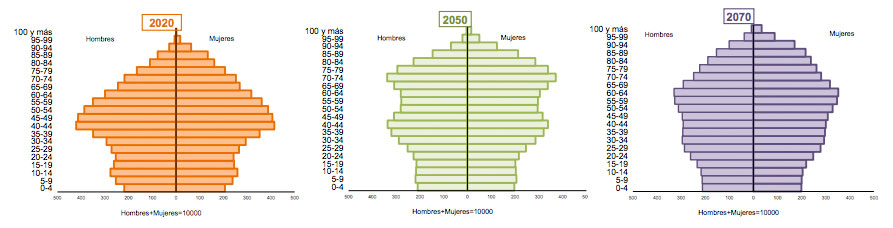
\includegraphics[width=0.98\textwidth]{imgs/piramide-poblacion.jpg}
    \caption{Pirámides de población de España en futuros años (\href{https://www.geriatricarea.com/2020/09/25/uno-de-cada-tres-espanoles-tendra-65-o-mas-anos-en-el-2050/}{geriatricarea.com})}
    \label{fig:piramide-poblacion}
\end{figure}

El aumento de la esperanza de vida de la población adulta en nuestro país ha supuesto que las personas mayores, muchas de ellas que viven solas y poseen nivel económico y cultural medio, supongan un sector amplio de la población que requiere de nuevas formas de ocio y de relacionarse socialmente. Muchas de estas personas viven solas y el sedentarismo y la falta de interacción social les produce que su desarrollo cognitivo se vea mermado.

También la frecuente automarginación de este grupo demográfico para el uso de herramientas digitales como juegos o aplicaciones, el fenómeno conocido de forma general como brecha digital, contribuye a un mayor aislamiento social. \enquote{Muchos adultos mayores tienen acceso a dispositivos móviles, pero no pueden aprovecharlos completamente debido a la falta de conocimiento o el miedo a salir de su zona de confort. Esto resulta en barreras emocionales, dificultades para adquirir nuevas habilidades tecnológicas} \parencite{intro1}. 

A pesar de lo mencionado en el párrafo anterior, el segmento de edad mayor de 60 años no es ajeno a la realidad de que las formas de socialización del siglo XXI están vinculadas a los avances tecnológicos y a las nuevas experiencias lúdicas. Como se señala en \textit{Las competencias digitales en personas mayores: de amenaza a oportunidad}: \enquote{el potencial que para las personas mayores ofrece el uso habitual de las TIC es enorme, con una larga lista de oportunidades existentes para el beneficio de este colectivo que deben ser aprovechadas} \parencite{intro4}.

Un juego digital que suponga entretenimiento para las personas mayores, al mismo tiempo que una mejora de memoria y ampliación de lenguaje y percepción puede significar un estimulante cambio en su día a día. 

\subsubsection{Impacto social y tecnológico de la pandemia de COVID-19}

Durante la pandemia por el COVID-19 millones de personas en el mundo tuvieron que pasar en pocos días de trabajo presencial al online y en sus relaciones personales debieron adaptar sus costumbres al nuevo escenario virtual.

De esta manera, personas acostumbradas a comunicarse solo por llamadas telefónicas, y muy poco mediante telefonía móvil, se volvieron usuarias de videollamadas diarias ante la necesidad de mantenerse conectados con familiares y amigos, combinada con las restricciones de movimiento.

Este cambio tuvo un impacto profundo en la vida diaria de las personas mayores. Por un lado, les brindó una forma vital de mantenerse conectados con sus seres queridos, incluso cuando no podían reunirse físicamente debido a las medidas de distanciamiento social. Esto ayudó a reducir un poco el riesgo de aislamiento social y proporcionó un medio para el apoyo emocional y la interacción social, lo cual es esencial para su bienestar mental y emocional.

Sin embargo, la transición a las tecnologías digitales también presentó desafíos, especialmente para aquellos menos familiarizados con ellas. Algunos enfrentaron dificultades técnicas al principio, como la configuración de aplicaciones o la resolución de problemas de conexión. Además, la dependencia excesiva de la tecnología para la comunicación también puede aumentar la brecha digital entre aquellos que tienen acceso y conocimientos tecnológicos y aquellos que no los tienen, lo que potencialmente podría aumentar el riesgo de exclusión social para algunos adultos mayores.

A pesar de estos desafíos, la pandemia actuó como un catalizador para la adopción de tecnología entre las personas mayores, lo que les permitió permanecer conectados y participar en la sociedad de manera más activa, incluso en tiempos de crisis. Como resultado, muchas personas mayores han incorporado el uso de tecnologías digitales en su vida diaria incluso después de que levantaran las restricciones de la pandemia, lo que les brinda nuevas oportunidades de participación social y acceso a recursos y servicios en línea \parencite{intro2}.

\subsection{Objetivos}
El presente trabajo tiene como objetivo principal concebir, desarrollar y evaluar un juego digital como contribución al desarrollo de soluciones innovadoras y efectivas que aborden el problema del aislamiento social en las personas mayores.

Este juego no solo buscará proporcionar entretenimiento y diversión, sino que también se centrará en promover la interacción social, el compromiso cognitivo y emocional, y en general, mejorar la calidad de vida de las personas mayores.
Para lograr este objetivo principal, se puede descomponer en varios subobjetivos más específicos que vienen ilustrados en la siguiente tabla:

\newpage
\begin{table}[t]
  \centering
  \begin{tabular}{| c | p{9.6cm} |}
    \hline
    \textbf{Subobjetivo} & \textbf{Descripción} \\
    \hline
    1. Revisión de la literatura & 
        1.1. Identificar las investigaciones clave sobre el impacto del aislamiento social en personas mayores \newline
        \vspace{0.2cm}
        1.2. Analizar la diversidad de intervenciones digitales dirigidas a este grupo demográfico \vspace{0.2cm} \\
    \hline
    2. Diseño del juego &
        2.1. Investigar las mejores prácticas en el diseño de juegos digitales accesibles para personas mayores \newline
        \vspace{0.2cm}
        2.2. Considerar las adaptaciones necesarias para abordar posibles limitaciones físicas y cognitivas
        \vspace{0.2cm} \\
    \hline
    3. Desarrollo técnico & 
        3.1. Seleccionar la plataforma y tecnologías más apropiadas para el desarrollo del juego \newline
        \vspace{0.2cm}
        3.2. Asegurar la compatibilidad con dispositivos comunes utilizados por personas mayores \newline
        \vspace{0.2cm}
        3.3. Integrar funcionalidades de accesibilidad, como ajustes de tamaño de fuente y navegación simplificada \vspace{0.2cm} \\
    \hline
    4. Contribución al conocimiento & 
    4.1. Contribuir al creciente cuerpo de conocimientos sobre cómo la tecnología puede mejorar la calidad de vida de las personas mayores, particularmente en el contexto del aislamiento social. 
    \vspace{0.2cm} \\
    \hline
    5. Participación comunitaria (TBD) & 
        5.1. Colaborar con comunidades de personas mayores para obtener retroalimentación durante el desarrollo del juego. \newline
        \vspace{0.2cm}
        5.2. Organizar pruebas piloto y grupos de enfoque para evaluar la experiencia del usuario. \vspace{0.2cm} \\
    \hline
    \end{tabular}
  \caption{Subobjetivos del trabajo.}
  \label{tab:subobjetivos}
\end{table}

\newpage
\section{Estado del arte}

En la intersección entre el avance tecnológico y el envejecimiento de la población, los juegos digitales emergen como una herramienta multifacética con el potencial de promover el bienestar y la calidad de vida de los adultos mayores. El estado del arte representa una síntesis dinámica de la investigación, desarrollo y aplicaciones existentes en este campo en constante evolución.

En esta revisión, se explorarán las principales tendencias y avances en cuatro áreas clave: los juegos serios, diseñados con objetivos específicos de aprendizaje o rehabilitación; los juegos digitales, adaptados para satisfacer las necesidades y preferencias de las personas mayores; el estado actual de las tecnologías aplicadas, incluyendo dispositivos y software especializado en el diseño y finalmente, ejemplos de aplicaciones prácticas desarrolladas en esta línea de investigación.

\subsection{Juegos serios}

Los juegos \textit{serios} se distinguen por su enfoque principal en objetivos educativos o formativos, relegando la diversión a un segundo plano \parencite{juegosSerios}.
Mientras que los juegos tradicionales buscan principalmente entretener al jugador, los juegos serios utilizan la pedagogía para integrar la instrucción dentro de la experiencia de juego. Esto implica que, aunque la diversión sigue siendo un elemento presente, el aprendizaje se convierte en el objetivo primordial.

\subsubsection{Origen de los juegos serios}

Hay que remontarse al año 1970 para datar la fecha de aparición del término juego serio o \textit{serious game}. En el contexto de los juegos de mesa, Clark Abt, investigador de EEUU publicó un libro titulado \enquote{\textit{Serious Games}} \parencite{juegosSerios5}, en el que explora las formas en que los juegos pueden utilizarse para instruir e informar. Utiliza enfoques innovadores para la resolución de problemas mediante técnicas de juego en contextos tan diferentes como el aprendizaje de las matemáticas, ciencias sociales y física o las tareas de planificación en el gobierno y la industria.

Pero no es hasta 2002 cuando el concepto de juego serio, tal como se conoce hoy en día, se recoge por Ben Sawyer
y David Rejeski en un artículo sobre los juegos serios en el ámbito de la política pública \parencite{juegosSerios6}, que tuvo un gran impacto, gracias a la creación de una asociación para promover el uso de los videojuegos con un propósito serio. Dicha asociación, Serious Games Initiative, de la cuál es cofundador Sawyer a través del Woodrow Wilson Center continúa activa en la actualidad \parencite{juegosSerios4}.

Precisamente, es Ben Sawyer quien establece como primer juego serio el videojuego America’s Army \parencite{juegosSerios7}, un simulador de combate para instruir a militares en el campo de batalla a través de la realización de diferentes misiones.


\subsubsection{Concepto de juego serio}
Los juegos serios son una categoría de videojuegos desarrollados principalmente para propósitos educativos y formativos, aunque también pueden tener elementos de entretenimiento. Estos juegos se distinguen por su enfoque en la transmisión de conocimientos y habilidades, a menudo relacionados con temas como la política, la salud, el entrenamiento militar, la educación, el ámbito empresarial, etc  \parencite{juegosSerios3}.

Se listan a continuación algunas de las características principales que distinguen a los juegos serios del resto:

\begin{itemize}[leftmargin=1.5cm, topsep=0pt, itemsep=1pt, after=\vspace{0pt}]
    \item \textbf{Fin educativo}: su principal objetivo es la formación en lugar del entretenimiento. La adquisición de habilidades técnicas y comprensión de procesos complejos.
    \item \textbf{Realismo}: están vinculados a aspectos de la realidad, favoreciendo la identificación del jugador con el contexto que se está simulando.
    \item \textbf{Ambiente virtual seguro}: proporcionan un entorno tridimensional virtual seguro para la práctica en ciertas áreas, como el entrenamiento militar.
    \item \textbf{Interés temático}: pueden abordar temas políticos, económicos, psicológicos, religiosos, entre otros, a menudo con un enfoque en la educación y el entrenamiento.
\end{itemize}

Los siguientes son algunos ejemplos reales y de ámbito específico de videojuegos serios:
\begin{itemize}[leftmargin=1.5cm, topsep=2.2pt, itemsep=1pt]
    \item \textbf{Biomedical Training}: entrenamiento para trabajadores de la salud en emergencias.
    \item \textbf{Food Force}: educación sobre el Programa Mundial de Alimentos de la ONU.
    \item \textbf{Incident Commander}: dirección de acciones en crisis sociales y desastres naturales.
    \item \textbf{Hazmat: Hotzone}: simulación para bomberos en situaciones de emergencia.
    \item \textbf{Yourselfittness}: regímenes de ejercicios físicos y aeróbicos.
    \item \textbf{Real Life 2007}: simulación global para entender condiciones de vida en diferentes países.
\end{itemize}

Los juegos serios son una herramienta poderosa para el aprendizaje y la formación en distintos campos. Involucran principios pedagógicos y cognitivos para garantizar un entrenamiento efectivo y ofrecen diversas ventajas como la familiarización con interfaces tecnológicas y la mejora de habilidades necesarias para la sociedad digital.

En el contexto de los adultos mayores, los videojuegos serios pueden resultar valiosos para el mantenimiento cognitivo, la estimulación mental y la mejora de habilidades específicas.

\newpage
\subsubsection{Juegos serios en la rehabilitación neuropsicológica}

Cabe destacar el papel de los juegos serios en el ámbito de la informática médica, en concreto, en el entrenamiento y la rehabilitación neuropsicológica. \enquote{En la rehabilitación cognitiva los retos de un juego serio por lo general inciden directamente en un déficit específico, lo que puede repercutir al mismo tiempo en más de uno} \parencite{juegosSerios2}.

En los últimos años, ha habido un notable aumento en la investigación y desarrollo de juegos computarizados para la rehabilitación cognitiva. Ejemplos como RehaCom® y Gradior® \parencite{ICTestudios} han demostrado resultados positivos en varios centros de salud al ofrecer una variedad de ejercicios digitales que abordan áreas cognitivas clave como la atención, la percepción, la memoria y el lenguaje.

En los centros de Salud Mental de la Fundación Rey Ardid en Zaragoza, se llevó a cabo la implementación de \textit{Gradior Suite} \parencite{reyardid}, un programa de evaluación y rehabilitación con más de trece mil actividades disponibles para personas a las que se ha detectado un deterioro cognitivo. Este software multiplataforma es ideal por su movilidad, capacidad de funcionar en línea u offline, y por disponer de planificaciones de ejercicios personalizables que pueden realizarse tanto con ratón como de forma táctil. 

Se muestran dos ejemplos de ejercicios: en la \autoref{fig:gradior-1}, la persona usuaria debe pulsar la tecla con la letra que dicte el juego y en la \autoref{fig:gradior-2}, hay que ir pulsado cada imagen en el orden correcto, siguiendo una secuencia de eventos lógica.

\begin{figure}[H]
    \centering
    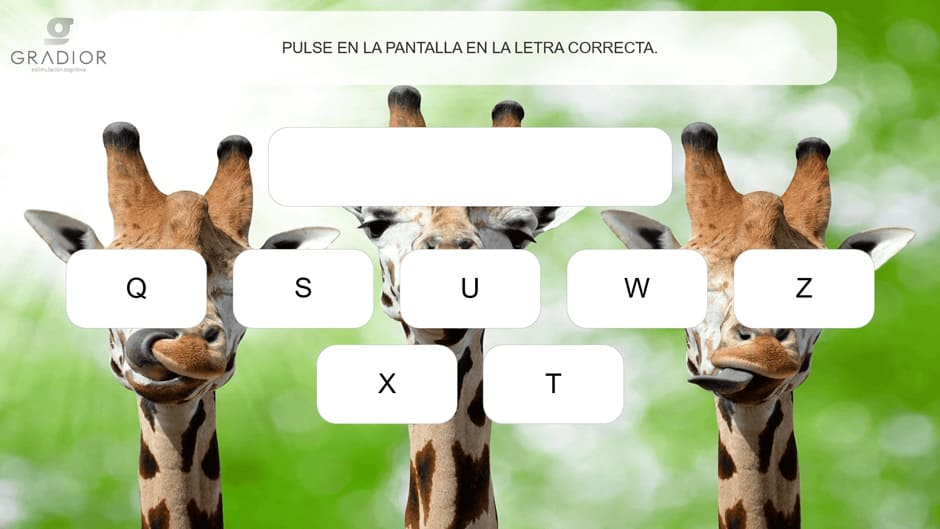
\includegraphics[width=0.6\textwidth]{imgs/gradior.jpg}
    \caption{Ejercicio de pulsar la letra correcta en Gradior}
    \label{fig:gradior-1}
\end{figure}

\begin{figure}[H]
	\centering
	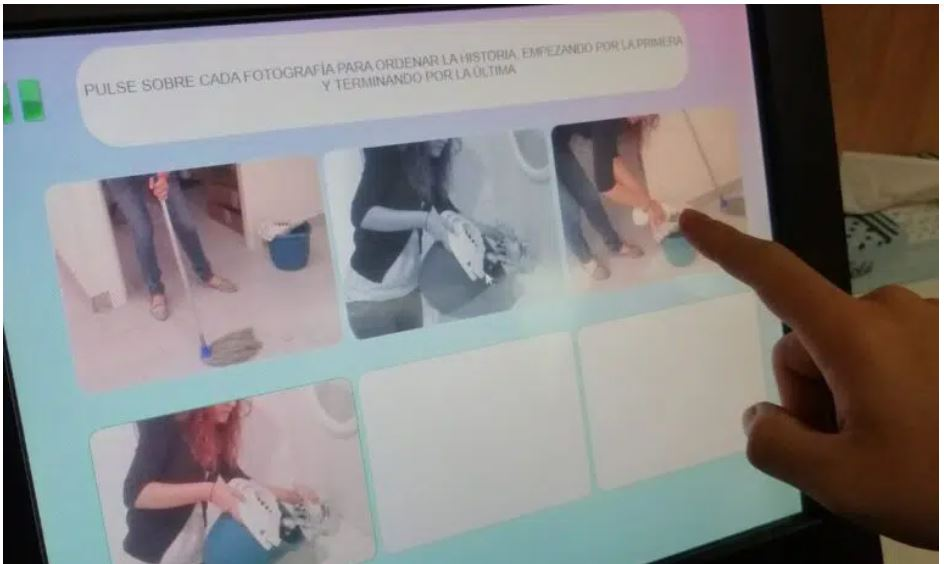
\includegraphics[width=0.6\textwidth]{imgs/gradior-2.jpg}
	\caption{Ejercicio de indicar el orden de imágenes correcto en Gradior}
	\label{fig:gradior-2}
\end{figure}

Otro destacado ejemplo es el módulo EINK de RehaCom® \parencite{hasomed2024}, diseñado para tratar déficits de memoria de trabajo y planificación mediante la simulación de situaciones diarias, como ir de compras. 

En la actividad, se le da al paciente una lista de productos para colocar en un carrito de compras. Al superar un cierto nivel de dificultad, el ejercicio incorpora cálculos matemáticos, ya que el paciente debe ajustar su compra a un presupuesto fijo y los precios de los artículos están indicados. Dicho entrenamiento se basa en alrededor de 100 fotografías realistas de productos y utiliza una salida de voz para nombrar los artículos seleccionados (\autoref{fig:eink}).

\begin{figure}[H]
	\centering
	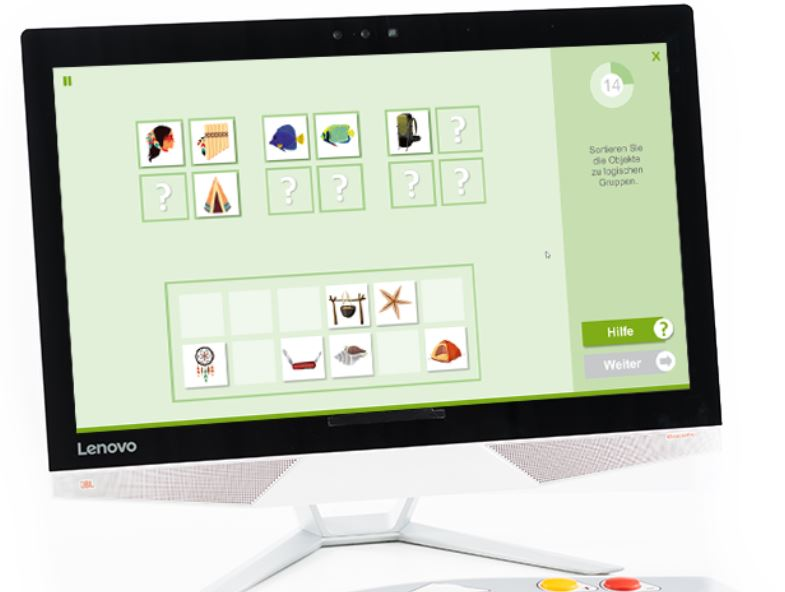
\includegraphics[width=0.6\textwidth]{imgs/EINK.jpg}
	\caption{Ejercicio de hacer la compra del módulo EINK de Rehacom}
	\label{fig:eink}
\end{figure}

En resumen, los juegos serios ofrecen una vía innovadora y efectiva para abordar las deficiencias cognitivas, a la vez que mantienen la motivación del paciente durante las sesiones de tratamiento.

\newpage
\subsubsection{Juegos tradicionales en grupo y sus ventajas cognitivas}

A continuación, se nombrarán algunos juegos tradicionales y populares que fomentan el contacto social y evitan el deterioro cognitivo en personas mayores, especialmente trabajando la memoria. Dado que esto es justo lo que se busca lograr con este proyecto, estas actividades servirán como fuente de inspiración para la conceptualización y desarrollo del mismo \parencite{juegosMem2}.

\begin{itemize}[leftmargin=1.5cm, topsep=2.2pt, itemsep=0.5pt]
    \item \textbf{Cada oveja con su pareja}: 
    consiste en agrupar objetos en función de su categoría, utilizando todo tipo de elementos. Desde las cartas de una baraja para agrupar por palos, hasta objetos aleatorios dispuestos, como frutas, verduras... Contribuye a mantener la capacidad intelectual, la memoria y la coordinación visual y manual.
    \item \textbf{Veo-veo}:
    juego mítico que hace las delicias de los más pequeños, y suele ser cuando juegan con alguien más mayor. Uno de los jugadores tendrá que adivinar el objeto elegido por su inicial; se pueden dar pistas sobre el lugar de la sala en que se encuentra.
    \item \textbf{Palabras encadenadas}:
    se trata de coger la última sílaba de una palabra y encadenar con la siguiente; que la última sílaba de esa palabra sea la primera de la siguiente. Fomenta la memoria y la comunicación, además de la atención y la concentración.
    \item \textbf{Puzzle de refranes}: 
    los adultos mayores son grandes conocedores de refranes populares. El juego consistirá en escribir los refranes en dos partes, en trozos de papel separados. Los jugadores deberán enlazar cada parte para completar el refrán, que puede ir orientado a una temática y luego formar un mural.
    \item \textbf{Quién es quién}:
    cada persona es asignada una palabra que todos menos él conocen. Dicha persona tendrá que ir haciendo preguntas de sí o no hasta adivinar quién o qué es.
    \item \textbf{Adivina la canción}:
    se pueden tomar como referencia las canciones más escuchadas del tiempo en el que las personas mayores eran jóvenes. Se reproducirá la canción durante un corto espacio de tiempo y los participantes anotarán el nombre y artista de la canción. Agudeza auditiva, rapidez y capacidad de atención son algunos de sus beneficios.
\end{itemize}

También destacan juegos de mesa como el Scrabble (creatividad y habilidades lingüísticas), Dominó (planificación y estrategia), Bingo (atención y memoria a corto plazo), Pictionary (comunicación no verbal), rompecabezas (concentración y paciencia), etc \parencite{juegos-mesa}.

\subsection{Juegos digitales para adultos mayores}

Una vez explicado el concepto de juego serio y algunos ejemplos concretos, se hará hincapié en un tipo concreto del mismo: los juegos digitales, que deben su nombre a la tecnologías de digitalización en las que están basados.

Los juegos digitales representan una herramienta innovadora y prometedora para abordar los desafíos asociados con el envejecimiento activo y saludable expuestos anteriormente. A través de dispositivos como computadoras, tabletas, consolas de juegos y teléfonos inteligentes, los adultos mayores tienen acceso a una amplia variedad de experiencias de juego que pueden contribuir a su bienestar físico, cognitivo y social.

Muchos de los juegos digitales populares entre adultos mayores están basados en juegos tradicionales, pues la familiaridad de las dinámicas es un factor que contribuye a su popularidad. Ejemplos de aplicaciones:
\begin{itemize}[leftmargin=1.5cm, topsep=2.2pt, itemsep=0.4pt]
    \item \textbf{Sudoku}: el clásico juego de números ayuda a ejercitar la mente y la concentración.
    \item \textbf{Wordscapes}: búsqueda de palabras que desafía la agilidad mental y el vocabulario.
    \item \textbf{Candy Crush Saga}: niveles de rompecabezas que pueden ser adictivos y desafiantes.
    \item \textbf{Jigsaw Puzzles}: selecciones de rompecabezas virtuales de diferentes niveles de dificultad.
    \item \textbf{Solitaire}: versión digital del clásico juego de cartas, fácil de aprender y entretenido.
    \item \textbf{Peak – Brain Games and Training}: variedad de juegos diseñados para ejercitar diferentes áreas del cerebro.
    \item \textbf{Neurona App}: aplicación que pretende estimular atención, memoria, razonamiento y planificación de adultos mayores mediante diversos juegos.
    \item \textbf{Fit Brain Trainer}: cuenta con 360 juegos de agilidad mental, memoria, capacidad visual y de deducción.
    \item \textbf{NeuroNation}: capaz de personalizar el entrenamiento para cada usuario \parencite{juegosMem1}.
\end{itemize}

Estos juegos son populares entre adultos mayores debido a su accesibilidad, puesto que son apps que pueden ser descargadas fácilmente en dispositivos móviles y tablets; tienen capacidad para ejercitar la mente, ya que la mayoría estimulan partes del cerebro concretas (la memoria, atención y resolución de problemas) y ofrecen entretenimiento sin demasiada complejidad al tener mecánicas de juego bastante simples.

La investigación en este campo se centra en comprender cómo los juegos digitales pueden promover el envejecimiento activo al mantener la mente activa, mejorar la destreza manual y fomentar la interacción social. Además, se busca diseñar juegos que sean accesibles y atractivos para esta población, teniendo en cuenta las necesidades y preferencias específicas de los adultos mayores.

A medida que la tecnología avanza y la aceptación de los juegos digitales entre los adultos mayores aumenta, resulta importante explorar cómo estos juegos pueden desarrollarse e integrarse de manera efectiva para mejorar la calidad de vida de esta población.


\subsubsection{El proyecto WorthPlay}

En este campo de investigación, destaca, entre otros, el proyecto \textit{WorthPlay} \parencite{WorthPlay2012}, que se enfoca en la investigación y desarrollo de juegos digitales para personas mayores, con el propósito de promover un envejecimiento activo y saludable. En él se reconoce que las tecnologías de la información y la comunicación (TIC) tienen el potencial de reducir el aislamiento social y mejorar el bienestar físico y psicosocial de los adultos mayores.

Para asegurar la efectividad de los juegos digitales, se destaca la necesidad de entender qué aspectos hacen que un juego valga la pena para esta población. Esto implica considerar elementos educativos, de socialización y de entretenimiento, así como la diversidad de preferencias en cuanto a la jugabilidad y el formato del juego.

\enquote{El proyecto se basa en el campo de la Interacción Persona-Ordenador (IPO), que busca mejorar la experiencia del usuario con las TIC. Se identifican tres olas en la investigación de IPO, desde la ergonomía hasta la experiencia de usuario (UX). WorthPlay se sitúa en la tercera ola, centrándose en la experiencia de juego y la participación del usuario durante un período prolongado en entornos reales} \parencite{WorthPlay2012}.

La investigación también se enfoca en la inclusión social y la superación de barreras de accesibilidad, como la destreza cognitiva y motriz. Se reconocen los estereotipos negativos sobre los adultos mayores en el contexto de los juegos digitales, y se busca desafiar estos estereotipos a través del diseño participativo de juegos.

El proyecto WorthPlay sigue un enfoque parecido al de este proyecto, ya que se basa en investigar y desarrollar prototipos de juegos destinados al envejecimiento activo y saludable de las personas mayores. Concretamente, hace hincapié en los juegos cognitivos, que estimulan el pensamiento y aprendizaje, y los de socialización, promoviendo las interacciones dentro del juego. Estos dos son justamente los puntos clave en los que debe centrarse el juego a implementar.

Se espera que este enfoque, seguido tanto en el proyecto Worthplay como en el desarrollo de este TFG, genere resultados significativos, contribuyendo a una mejor comprensión de las necesidades y preferencias de los adultos mayores en este campo.

\subsubsection{El juego digital \textit{Solitaire Quizz}}

Esta investigación tenía como fin establecer una serie de criterios de accesibilidad y usabilidad para adultos mayores, en el contexto del diseño de juegos digitales que sirvan como herramienta de aprendizaje. Para ello, se evaluó una versión digital del tradicional juego de cartas del Solitario, llamada \textit{Solitaire Quiz}, disponible en varias plataformas como Android, iOS y web \parencite{diseño2017}.

La metodología del proyecto seguía un modelo de prototipado rápido, con un total de tres iteraciones, donde la última consistía en la evaluación de la experiencia de 42 usuarios con más de 55 años mediante tres cuestionarios de escala Likert, uno para cada apartado relevante a estudiar: diseño, usabilidad y legibilidad.

Este juego, además de la mecánica del original, incluye contenido de aprendizaje en forma de cuestionarios que se lanzan durante la partida (\autoref{fig:solitaire-2}), que además tienen una dificultad modificable, y ofrecen retroalimentación instantánea, sonora y visual, tanto si la respuesta es correcta como si no lo es.

\begin{figure}[H]
	\centering
	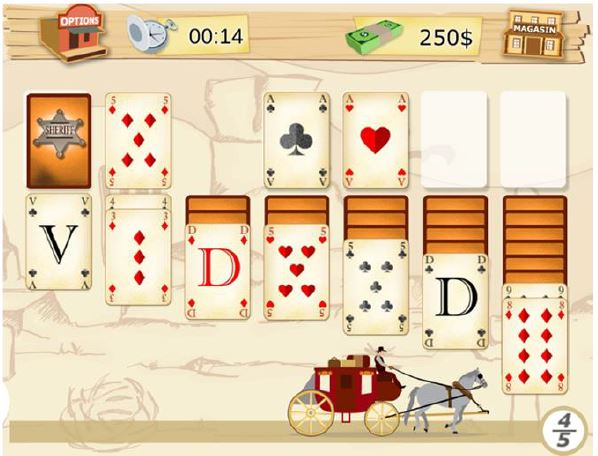
\includegraphics[width=0.7\textwidth]{imgs/solitaire-1.JPG}
	\caption{Pantalla del juego digital \textit{Solitaire Quiz}}
	\label{fig:solitaire-1}
\end{figure}

Algunos de los aspectos que hacen a este juego accesible al público al que va dirigido son: la simplificación de la interfaz (mostrada en la \autoref{fig:solitaire-1}), limitándose a imágenes representativas y evitando elementos distractorios; la asistencia activa del juego, que guía al usuario y evita que se quede estancado en alguna pregunta y la legibilidad de los textos y gráficos.

\begin{figure}[H]
	\centering
	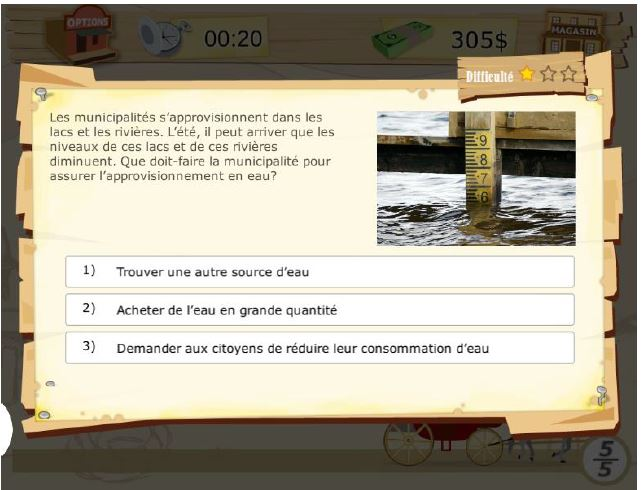
\includegraphics[width=0.7\textwidth]{imgs/solitaire-2.JPG}
	\caption{Evento de aprendizaje en \textit{Solitaire Quiz}}
	\label{fig:solitaire-2}
\end{figure}

Muchos de los parámetros estudiados han servido como base para la sección de cuestiones estéticas y usabilidad de este proyecto (\textit{5.4.3.}).

\subsection{Estado del arte de los asistentes virtuales}

En esta sección, se hablará sobre el estado actual de los asistentes virtuales, que se caracteriza por su creciente sofisticación impulsada por la IA, su diversidad en términos de funciones y aplicaciones, y la presencia destacada de plataformas líderes como Alexa, que continúan innovando y expandiendo las fronteras de esta tecnología.

\subsubsection{Influencia de la IA y clasificación}

La inteligencia artificial (IA) es una tecnología que ha evolucionado rápidamente y se ha integrado en la vida cotidiana de las personas, especialmente en la automatización de servicios y la toma de decisiones. Ha encontrado aplicaciones en diversos sectores, como la educación, la salud, la economía y la política, transformando la forma en que se prestan servicios y se interactúa con las organizaciones.

El aumento de la población y el crecimiento exponencial de las ciudades requieren sistemas más rápidos y eficientes para la atención al cliente. A raíz de esta necesidad, se han desarrollado asistentes virtuales inteligentes.

Un asistente virtual es un software con acceso a recursos en línea que emplea técnicas de IA y procesamiento del lenguaje natural para proporcionar soporte en tiempo real a usuarios y otorgar acceso a información relevante sobre los servicios ofrecidos por organizaciones públicas y privadas \parencite{tfgAlexa1}.

La arquitectura de estos sistemas se ha perfeccionado con el tiempo, desde ELIZA, precursor que emulaba a un psicoterapeuta, hasta los chatbots avanzados y versátiles de hoy en día, compatibles con múltiples dispositivos (altavoces, televisores, teléfonos móviles, tablets, etc).

En cuanto a la clasificación, existe más de un criterio para definir de los tipos de asistentes virtuales, pero los principales son los mencionados en el Cuadro \ref{tab:criterios_asistentes_virtuales}: según el grado de interacción con los usuarios, las funciones y finalidades del servicio, los medios de interacción y el grado de afectividad \parencite{asistentesConv}.

\begin{table}[H]
    \centering
    \begin{tabular}{|l|l|}
    \hline
    \rowcolor{lightgray}
    \textbf{Criterio} & \textbf{Tipos} \\
    \hline
    \multirow{2}{*}{Grado de interacción} & - Dirigidos \\
     & - Conversacionales \\
    \hline
    \multirow{3}{*}{Funciones y finalidades} & - Comunicación y marketing \\
     & - Atención al cliente \\
     & - Mejora de procesos \\
    \hline
    \multirow{3}{*}{Medios de interacción} & - Texto \\
     & - Multimedia \\
     & - Voz \\
    \hline
    \multirow{2}{*}{Grado de afectividad} & - No emocionales \\
     & - Emocionales \\
    \hline
    \end{tabular}
    \caption{Clasificación de asistentes virtuales}
    \label{tab:criterios_asistentes_virtuales}
\end{table}

\begin{itemize}[leftmargin=1.5cm, topsep=2pt, itemsep=1pt]
    \item \textbf{Dirigidos}: realizan preguntas predefinidas a los usuarios mediante elementos fijos, controlando la interacción con el usuario.
    \item \textbf{Conversacionales}: permiten una mayor libertad en las preguntas que el usuario quiere hacer, promoviendo una interacción más natural.
    \item \textbf{Comunicación y marketing}: brindan servicios de consulta dentro de aplicaciones móviles o web.
    \item \textbf{Atención al cliente}: asisten a los usuarios resolviendo sus dudas y consultas a través de conversaciones continuas.
    \item \textbf{Mejora de procesos}: tienen el objetivo de reducir el tiempo dedicado a una área específica.
    \item \textbf{No emocionales}: son los chatbots tradicionales y se limitan a dar respuestas oportunas a las solicitudes del usuario.
    \item \textbf{Emocionales}: diseñados para interactuar y comprender a las personas a través de conversaciones informales, permitiendo una atención personalizada.
\end{itemize}

Con respecto a las tendencias en el desarrollo e implementación de asistentes virtuales en organizaciones públicas y privadas, se observa que actualmente se utilizan asistentes dirigidos, el tipo más dominante es el de atención al cliente, el medio de interacción más empleado es el texto y suelen ser son no emocionales.

\subsubsection{Alexa, el asistente conversacional más extendido hoy en día}

Junto con Siri (Apple) y Google Assistant, Alexa, desarrollada por Amazon, es sin lugar a dudas una de los asistentes virtuales por voz más extendidas. Numerosos estudios confirman el creciente índice de uso e impacto en el mercado que ha supuesto el lanzamiento de Alexa, entre ellos los resultados obtenidos en la clasificación por puntuaciones del \textit{Voice Platform Impact Rating} (\autoref{fig:grafico-asistentes}).

\begin{figure}[H]
    \centering
    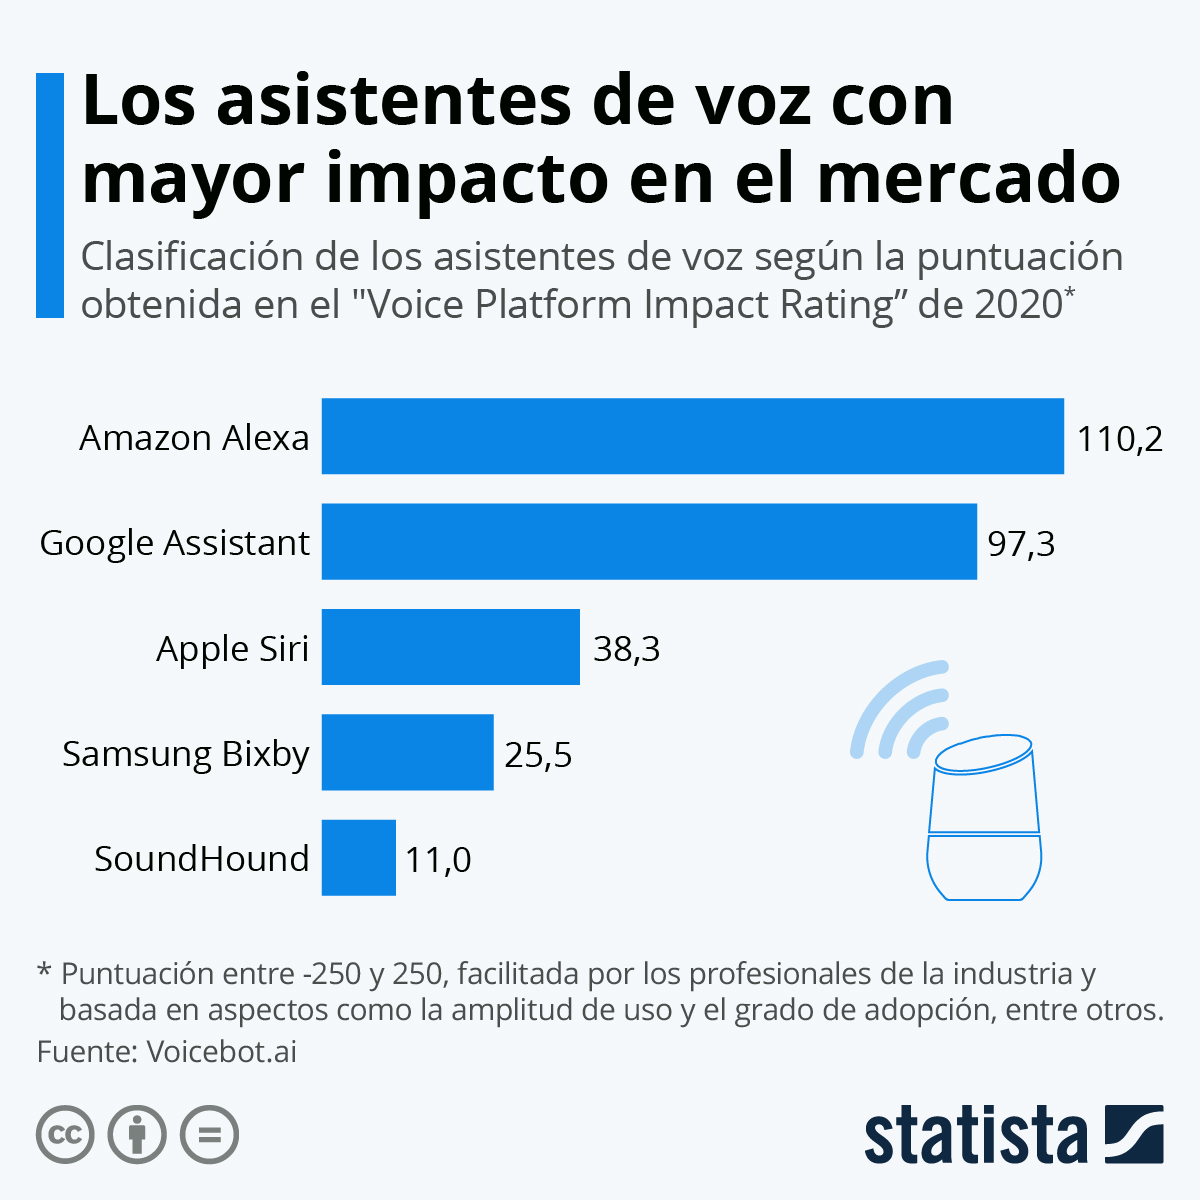
\includegraphics[width=0.5\textwidth]{imgs/grafico-asistentes.jpeg}
    \caption{Ranking de asistentes de voz según el VPIR en 2020 (\href{https://es.statista.com/grafico/22578/clasificacion-de-los-asistentes-de-voz/}{statista})}
    \label{fig:grafico-asistentes}
\end{figure}

Alexa fue lanzado en noviembre de 2014, se encuentra alojado en la nube de Amazon y está disponible en una gran variedad de dispositivos, incluyendo Amazon Echo y Echo Plus, así como también en dispositivos de terceros como smartphones, Raspberry Pi y vehículos.

Actualmente, cuenta con una amplia gama de funciones predefinidas, como manejo de alarmas, notificaciones, calendarios y búsqueda en internet para responder preguntas. Sin embargo, su verdadero potencial radica en las \textit{skills}, similares a aplicaciones de terceros que amplían sus funcionalidades, permitiendo interactuar con distintas compañías y acceder a sus servicios desde un mismo lugar. A nivel mundial, Alexa cuenta con más de 56,000 skills disponibles \parencite{tfgAlexa2}.

Las \textit{skills} de Alexa para el desarrollo de juegos ofrecen una amplia gama de posibilidades para crear experiencias interactivas y entretenidas. Estas habilidades permiten a los desarrolladores crear juegos de diferentes géneros y niveles de complejidad, desde simples juegos de palabras y adivinanzas hasta juegos de aventuras o trivial más elaborados.

Además, según estudios para determinar el <<mejor>> asistente de voz, como el realizado en la Universidad de Costa Rica con 92 estudiantes \parencite{berdasco2020evaluacion}, Alexa, junto con Google Assistant, lideran en cuanto a satisfacción del usuario frente a otros como Siri y Cortana, al haber obtenido los mejores resultados en relación con la calidad de las respuestas (\autoref{fig:grafico-alexa-1}) y su correctitud (\autoref{fig:grafico-alexa-2}) en la escala de Likert sobre cinco puntos.

\begin{figure}[H]
	\centering
	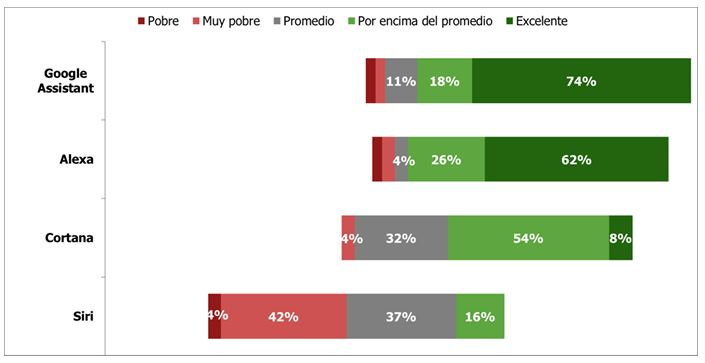
\includegraphics[width=0.7\textwidth]{imgs/alexa-compare-1.JPG}
	\caption{Resultados de la pregunta <<¿Qué tan buenas fueron las respuestas?>>}
	\label{fig:grafico-alexa-1}
\end{figure}

\begin{figure}[H]
	\centering
	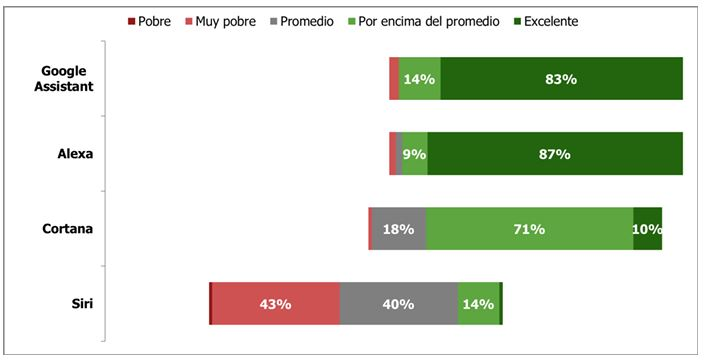
\includegraphics[width=0.7\textwidth]{imgs/alexa-compare-2.JPG}
	\caption{Resultados de la pregunta <<¿Qué tan correctas fueron las respuestas?>>}
	\label{fig:grafico-alexa-2}
\end{figure}

La calidad de respuesta es la percepción de las personas usuarios acerca de cómo de natural es la respuesta del asistente, para lo que se tiene en cuenta la claridad, el grado de detalle y la entonación. Por otro lado, la correctitud simplemente evalúa si la respuesta es verídica o no. En cuanto a las preguntas planteadas a los asistentes, abarcaban diversos temas como las ciencias, matemáticas, cultura general y tareas del día a día.

Una vez comprobado que Alexa es una buena opción, esimportante analizar la relación existente entre Alexa y el grupo demográfico al que va dirigido este proyecto.

\subsubsection{Las interacciones entre adultos mayores y Alexa}

En el artículo \textit{Análisis de la accesibilidad al altavoz inteligente Alexa en personas adultas mayores} \parencite{tello2023analisis}, primero se han identificado las barreras en el uso de asistentes de voz como Alexa por las personas mayores, entre las que destacan: las dificultades para aprender a utilizarlo, la percepción de pérdida de la independencia que pueden desarrollar algunos usuarios, la desmotivación por falta de confianza en sus habilidades tecnológicas, los posibles problemas cognitivos que puedan tener, etc.

No obstante, también se han descubierto beneficios del uso de Alexa para los adultos mayores, entre los cuales se encuentran: la promoción de la independencia, al recordar tareas cotidianas y controlar dispositivos del hogar; la reducción de la soledad, con funciones como la reproducción de música o aquellas relacionadas con el entretenimiento, el desarrollo de alternativas de comunicación con sus contactos... Además, puede ayudar a superar las barreras relacionadas con la falta de familiaridad de los adultos mayores con las tecnologías.

Cabe destacar que para poder alcanzar los beneficios anteriores, es preciso seguir algunas recomendaciones para la mejora de estas interacciones, en concreto se mencionan tres puntos clave:
\begin{itemize}
	\item \textbf{Diseño accesible}: aunque el modelo de interacción por voz ya sea considerado útil al evitar depender de habilidades motrices y visuales, se debe tratar de potenciar la accesibilidad a través de respuestas claras y personalizadas.
	\item \textbf{Ergonomía cognitiva}: siempre se debe intentar proporcionar indicaciones simples y fáciles de entender, para reducir el esfuerzo cognitivo requerido por las personas usuarias.
	\item \textbf{Educación tecnológica}: es importante promover la independencia de los adultos mayores, pero no se puede prescindir de una formación previa, para lo que es necesario guiar a los adultos mayores en su proceso de aprendizaje tecnológico. 
\end{itemize} 

En definitiva, Alexa tiene un gran potencial para promover el envejecimiento activo y saludable de las personas adultas mayores, siempre que se consideren las barreras de accesibilidad existentes y se implementan medidas para sobrepasarlas.

Por los motivos mencionados en esta sección y la anterior, se va a elegir a Alexa como la asistente virtual para el juego a desarrollar.

\subsection{Aplicaciones similares con asistentes de voz}

Se han visto algunas aplicaciones dirigidas a adultos mayores para favorecer su envejecimiento saludable en secciones anteriores, y ahora se mencionarán ejemplos de aplicaciones similares con asistentes conversacionales. 

\subsubsection{CELIA, mucho más que una asistente}

Existen algunas iniciativas dirigidas a las personas mayores que están en situación de aislamiento como el asistente virtual Celia (\href{https://celiatecuida.com/}{web oficial Celia}), desarrollado por personal del Centro de Investigación en Tecnologías de Telecomunicación de la Universidade de Vigo, atlanTTic, que ya se ha puesto en marcha con éxito ya que su uso es muy sencillo \parencite{celia-app}.

Las personas interesadas pueden acceder a este asistente virtual desde su teléfono móvil a través de la aplicación gratuita de CELIA (\autoref{fig:celia}), y también por WhatsApp, enviando un mensaje de texto o una nota de voz de manera que establecen una conversación con <<Celia>>. De esta sencilla manera  la persona  mayor que vive sola puede preguntar al asistente virtual al levantarse <<¿Qué tiempo va a hacer hoy?>> y buscar actividades para acudir como exposiciones, conferencias, conciertos que sean al aire libre o en espacios cubiertos dependiendo de la climatología. 

\begin{figure}[H]
    \centering
    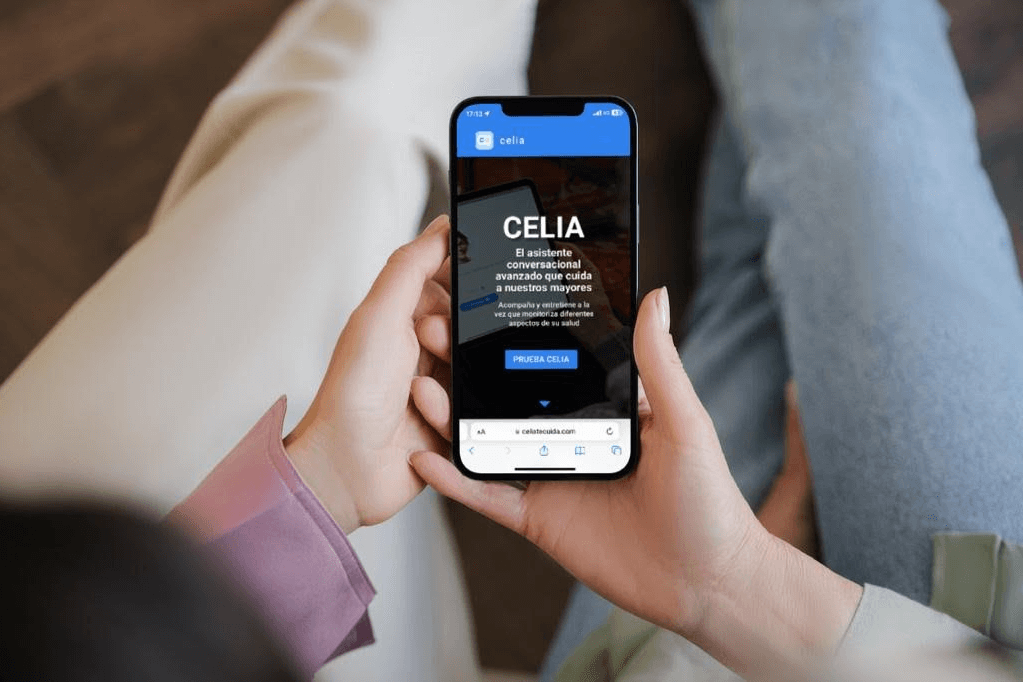
\includegraphics[width=0.55\textwidth]{imgs/celia.jpg}
    \caption{Celia, una asistente todoterreno 24 horas al día.}
    \label{fig:celia}
\end{figure}

Esta aplicación es útil para la ejecución de comandos básicos y ayuda a las personas mayores, pero no ofrece la capacidad de personalización de un juego digital centrado en promover el envejecimiento activo de los adultos mayores, además de no estar pensado para el uso de más de una persona a la vez.

\subsubsection{Juego de los trayectos orientado a la detección del deterioro cognitivo}

Es una aplicación (o skill) basada en Alexa que puede usarse como una herramienta clínica destinada a la evaluación de la capacidad de memoria de trabajo en pacientes. El juego implementado consiste en ir memorizando las calles de Jaén de una ruta seleccionada aleatoriamente del mapa cada vez que se inicia una partida \parencite{tfgAlexa3}.

Es compatible y accesible a través de cualquier dispositivo de la familia de Alexa y viene con un sistema robusto de almacenamiento en la nube, diseñado para almacenar de manera segura y eficiente toda la información de los usuarios y sus interacciones con el sistema.

El juego en sí consiste en que la persona usuaria, un adulto mayor, debe recordar secuencias en forma de nombres de calle, contestando a las preguntas formuladas por Alexa, quien es la encargada de pedirle nombres de calles o rutas para ejercitar su memoria. Se incluye un ejemplo de ejecución el la \autoref{fig:tfg-caminos-1}.

\begin{figure}[H]
	\centering
	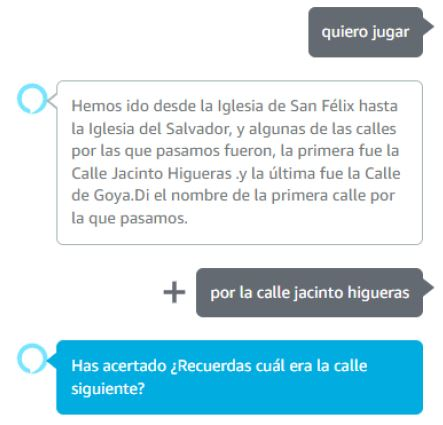
\includegraphics[width=0.5\textwidth]{imgs/tfg-caminos-1.JPG}
	\caption{Ejemplo de interacción con el juego de las rutas}
	\label{fig:tfg-caminos-1}
\end{figure}

Además, en los dispostivos de Alexa conn pantalla, se mostrará un soporte visual con imágenes de las calles para ayudar y hacer el juego más atractivo (\autoref{fig:tfg-caminos-2}).

\begin{figure}[H]
	\centering
	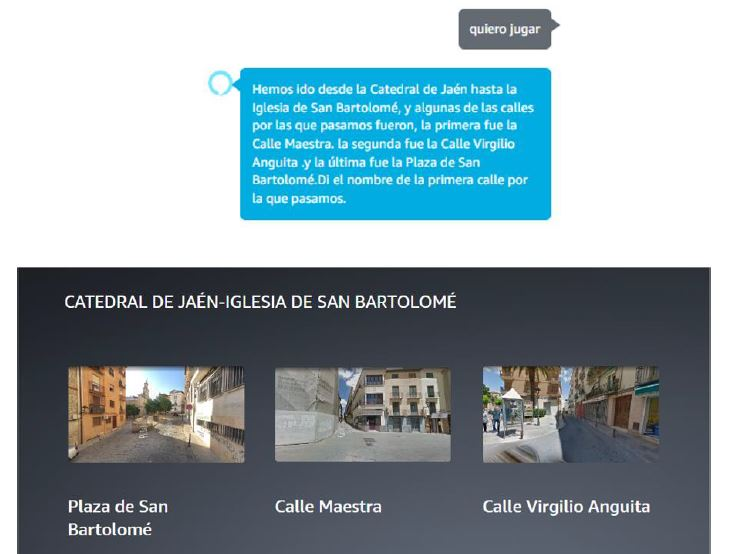
\includegraphics[width=0.75\textwidth]{imgs/tfg-caminos-2.JPG}
	\caption{Interacción con el juego de las rutas y su interfaz}
	\label{fig:tfg-caminos-2}
\end{figure}

\newpage
Los resultados de las partidas y la información de los usuarios se almacenan en una base de datos y pueden ser consultados mediante una app complementaria, destinada exclusivamente al uso del especialista. Así, este último podrá evaluar de manera efectiva la capacidad de memoria de trabajo de sus pacientes, facilitando la detección rápida del deterioro cognitivo.

En cuanto a la estimulación cognitiva y accesibilidad, es una aplicación sólida y une buena fuente de inspiración para este proyecto; sin embargo, se echa en falta el aspecto social del juego, ya que está pensado para un solo jugador o jugadora. La aplicación a desarrollar en este proyecto sí tendrá en cuenta este factor, considerando no solo beneficios cognitivos, sino también vinculados a las relaciones sociales.

\subsubsection{Juegos serios y experiencias inclusivas}

El proyecto \enquote{Juegos serios y experiencias inclusivas} \parencite{tfgAlexa4} tiene como objetivo desarrollar dos juegos serios que promuevan el envejecimiento activo y el ejercicio cognitivo para personas mayores, utilizando el asistente de voz Alexa. Estos juegos están diseñados para ser accesibles y permitiendo que los participantes ejerciten sus habilidades cognitivas a la vez que se entretienen. A continuación, se describen los dos juegos desarrollados:

El primero, series de palabras, consiste en que el usuario debe recordar y repetir una serie de palabras que Alexa le dicta. Cada vez que repite correctamente la secuencia, se le añade una nueva palabra. Estas listas incluyen temas como colores, animales, países o una mezcla de los anteriores. Se muestra un ejemplo de partida en la \autoref{fig:tfg-juegos-1} y \ref{fig:tfg-juegos-11}: 

\begin{figure}[H]
	\centering
	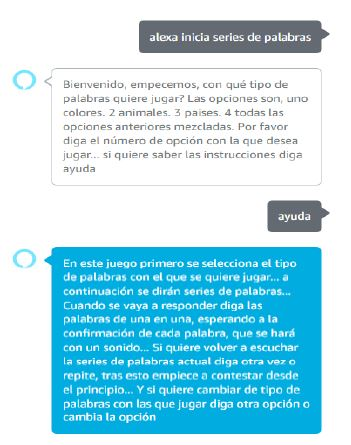
\includegraphics[width=0.5\textwidth]{imgs/tfg-juegos-1.JPG}
	\caption{Interacción con el juego de las series de palabras (1)}
	\label{fig:tfg-juegos-1}
\end{figure}

\begin{figure}[H]
	\centering
	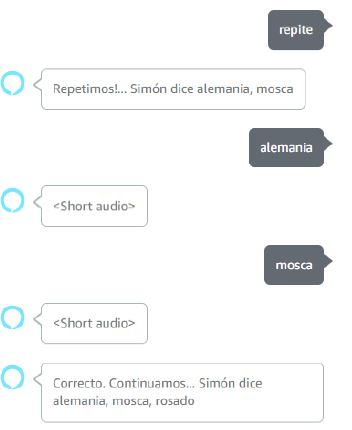
\includegraphics[width=0.45\textwidth]{imgs/tfg-juegos-11.JPG}
	\caption{Interacción con el juego de las series de palabras (2)}
	\label{fig:tfg-juegos-11}
\end{figure}

En el segundo juego (\autoref{fig:tfg-juegos-2}), Alexa plantea afirmaciones sobre diversos temas de cultura general, y el jugador debe responder si la afirmación es verdadera o falsa. Si el jugador tiene dudas, puede pedir una pista o saltarse la pregunta. Tras la respuesta, Alexa proporciona una breve explicación sobre la afirmación, tanto si fue correcta como incorrecta.

\begin{figure}[H]
	\centering
	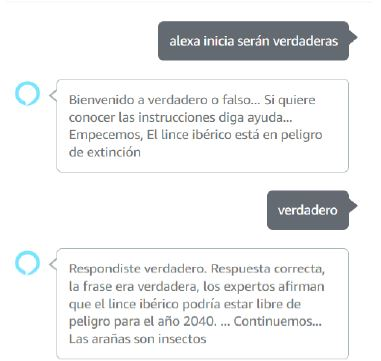
\includegraphics[width=0.5\textwidth]{imgs/tfg-juegos-2.JPG}
	\caption{Interacción con el juego de verdadero o falso}
	\label{fig:tfg-juegos-2}
\end{figure}

Como sucedía con la aplicación anterior, si bien es cierto que estos juegos ayudan a estimular la memoria tanto a corto plazo como largo, así como la concentración y razonamiento, no consideran la modalidad multijugador que podría beneficiar a su envejecimiento saludable.


\newpage
\section{Planificación, metodología y presupuesto}

En esta sección, se van a definir los componentes fundamentales en la gestión del proyecto que nos permitirá desarrollar una aplicación en Alexa para mejorar las habilidades cognitivas y sociales de los adultos mayores a través del entretenimiento en residencias y centros de día.

\subsection{Planificación temporal}

Se ha elaborado un calendario, marcando con colores los plazos (en días) de las distintas tareas y subtareas en las que se ha desglosado el proyecto (\autoref{fig:planning1} y \ref{fig:planning2}.

\begin{figure}[H]
	\centering
	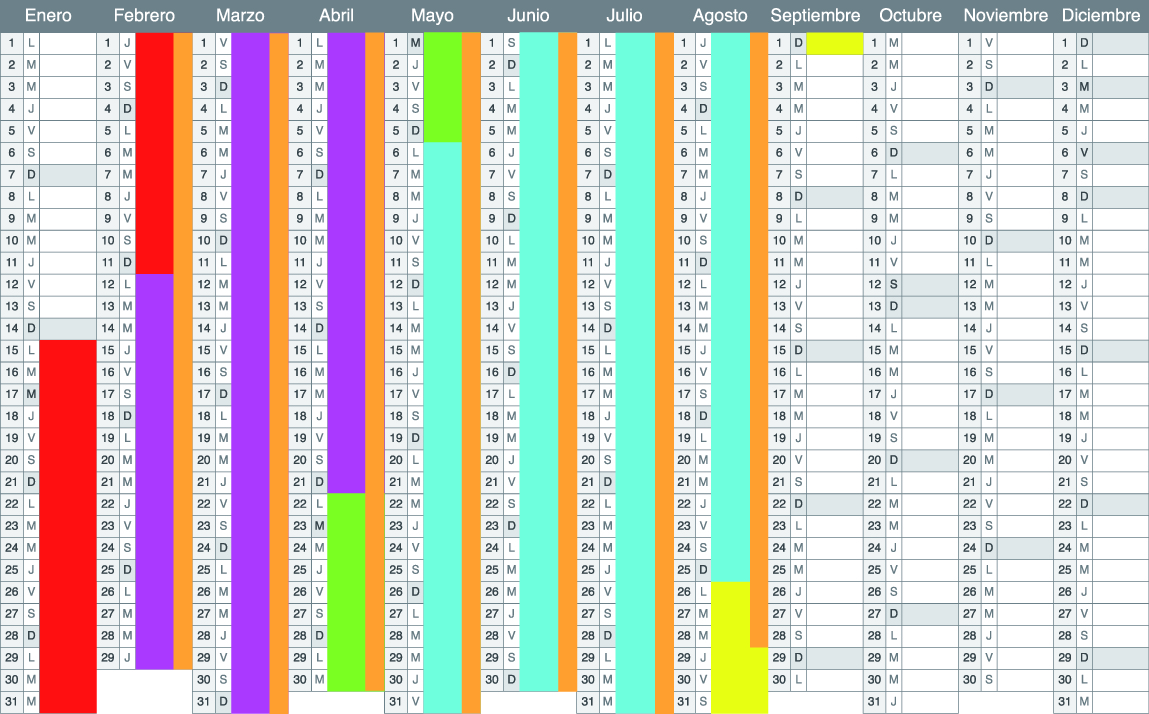
\includegraphics[width=1\textwidth]{imgs/tabla-planning1.jpg}
	\caption{Planificación temporal en el calendario}
	\label{fig:planning1}
\end{figure}

\begin{figure}[H]
	\centering
	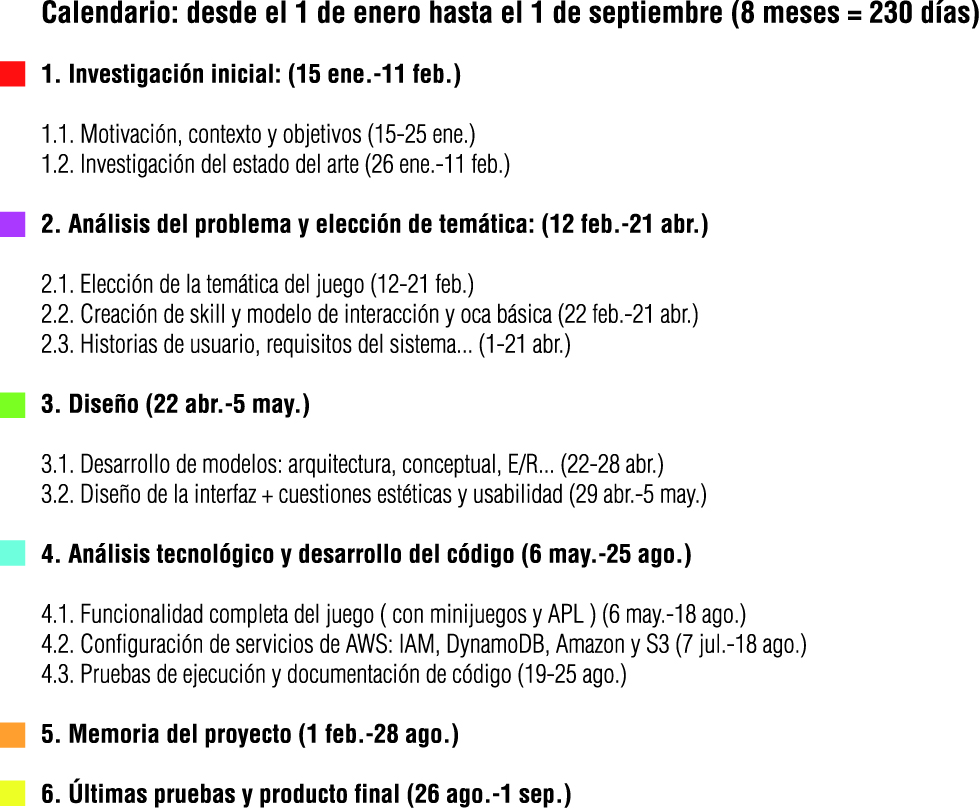
\includegraphics[width=1\textwidth]{imgs/tabla-planning2.jpg}
	\caption{Leyenda de la planificación temporal por (sub)tareas}
	\label{fig:planning2}
\end{figure}

Por tanto, si de esos 230 días que se ha estado trabajando en este proyecto, se estima que las horas empleadas cada día de media son 2'5, entonces se habrán dedicado cerca de 600 horas en total.

\newpage

\subsection{Metodología}

La metodología de desarrollo describe las técnicas y procesos que se seguirán para desarrollar el proyecto, incluyendo los roles y responsabilidades del equipo y los métodos de comunicación y gestión del proyecto. En este caso, se va a seguir un \textit{modelo evolutivo basado en prototipos} \parencite{carr1997prototyping}.

Este modelo incorpora el concepto de prototipos, entendidos como versiones preliminares del sistema que ayudan a refinar los requisitos y funcionalidades del mismo, mediante interacciones con los clientes y/o personas usuarias, antes del desarrollo del producto final.

En este caso, se tratará de un modelo evolutivo, ya que el enfoque se basa en ir construyendo y refinando una versión inicial del software en ciclos iterativos, adaptándose a los distintos cambios y necesidades hasta llegar a un producto final. La participación continua de los clientes y el carácter gradual del modelo permite flexibilidad a la hora de mejorarlo, y la posibilidad de definir requisitos no estáticos.

Todo modelo de prototipos se descompone en las siguientes fases, mostradas en la \autoref{fig:modelo-prototipos}:

\begin{figure}[H]
	\centering
	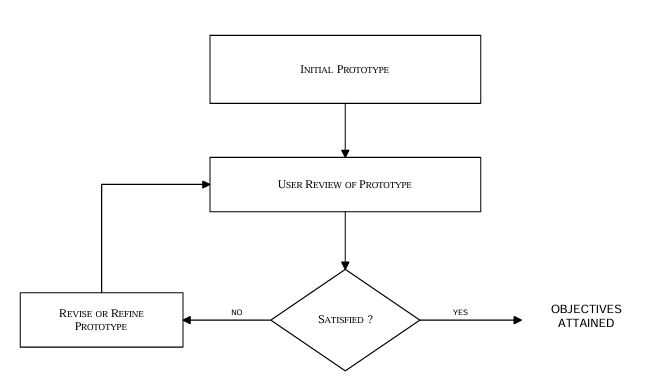
\includegraphics[width=0.8\textwidth]{imgs/modelo-prototipos.JPG}
	\caption{El proceso de desarrollo de prototipos \parencite{carr1997prototyping}}
	\label{fig:modelo-prototipos}
\end{figure}

\begin{enumerate}
    \item \textbf{Identificar los requisitos básicos}: previo al desarrollo de cualquier prototipo, se deben establecer las necesidades básicas en forma de requisitos funcionales, que pueden no estar completos del todo ya que se mejorarán en las siguientes fases.
    \item \textbf{Prototipo inicial}: se desarrolla una versión básica del software, centrándose en los aspectos relevantes de los requisitos establecidos anteriormente.
    \item \textbf{Revisión del usuario del prototipo}: los clientes y/o usuarios realizan pruebas sobre el prototipo, permitiendo detectar fallos o posibles mejoras en sus funcionalidades.
    \item \textbf{Revisión de requisitos y refinamiento}: en base a la retroalimentación de la fase anterior, se amplían o modifican las funcionalidades en una serie de ciclos iterativos, mejorando de forma gradual el prototipo inicial.
    \item \textbf{Aceptación/finalización}: una vez se ha terminado de revisar y refinar, se puede concluir que el prototipo satisface los requisitos establecidos, y por tanto, se ha logrado obtener el producto final.
\end{enumerate}


\subsection{Presupuesto}

El presupuesto permite gestionar los recursos del proyecto, desde el asignamiento de recursos humanos hasta la adquisición de equipamiento y materiales necesarios.

\subsubsection{Recursos humanos}
Los recursos humanos incluyen a las personas involucradas en el proyecto, tanto en las etapas previas al desarrollo como durante el mismo. 

Los datos de esta tabla han sido calculados a partir de las tablas salariales por titulación en España \parencite{glassdoor2024}.  

\begin{table}[H]
    \centering
    \begin{tabular}{|c|c|c|c|c|}
    \hline
    \rowcolor{lightgray}
    \textbf{Descripción} & \textbf{Horas} & \textbf{€/año} & \textbf{€/h} & \textbf{Coste (€)} \\
    \hline
    Desarrollador(a) de software & 300 & 33.750 & 16,23 & 4.869 \\
    \hline
    Ingeniero/a de Cloud Computing & 72 & 42.507 & 20,44 & 1.471,68 \\
    \hline
    Psicólogo/a & 10 & 23.794 & 12,20 & 122 \\
    \hline
    Expertos en Gerontología de la UGR & \multicolumn{4}{|c|}{Colaboración voluntaria} \\
    \hline
    \textbf{Total} & \textbf{382} & \multicolumn{2}{|c|}{} & \textbf{6.462,68} \\
    \hline
    \end{tabular}
    \caption{Presupuesto para recursos humanos}
    \label{tab:presupuesto-personal}
\end{table}

\subsubsection{Hardware}
La parte de hardware son todos los dispositivos físicos y electrónicos necesarios para llevar a cabo la aplicación.

El coste mensual del dispositivo se calcula dividiendo el precio original entre su vida útil (en meses), y después esa cantidad se puede multiplicar por el número de meses que se ha utilizado para hallar el importe amortizado.

\begin{table}[H]
    \centering
    \begin{tabular}{|c|c|c|c|c|}
    \hline
    \rowcolor{lightgray}
    \textbf{Descripción} & \textbf{Precio (€)} & \textbf{Vida útil (meses}) & \textbf{Uso (meses)} & \textbf{Importe amortizado (€)}\\
    \hline
    HP 15s Intel Core i5 & 650 & 72 & 8 & 72,24 \\
    \hline
    Amazon Echo Show 5 & 70 & 60 & 9 & 9,36 \\
    \hline
    \multicolumn{4}{|c|}{\textbf{Total}} & \textbf{81,6} \\
    \hline
    \end{tabular}
    \caption{Presupuesto para hardware}
    \label{tab:presupuesto-hw}
\end{table}

\subsubsection{Software}
La parte de software está constituida por todos los programas utilizados durante el proceso, desde el análisis y diseño hasta el desarrollo y despliegue.  

\begin{table}[H]
    \centering
    \begin{tabular}{|c|c|}
    \hline
    \rowcolor{lightgray}
    \textbf{Descripción} & \textbf{Coste (€)}\\
    \hline
    Visual Paradigm & Licencia académica gratuita \\
    \hline
    Amazon Web Services (AWS) & 10 \\
    \hline
    TeXstudio & 0 \\
    \hline
    Visual Studio Code & 0 \\
    \hline
    GitHub & 0 \\
    \hline
    Alexa Developer Console & 0 \\
    \hline
    \textbf{Total} & \textbf{10} \\
    \hline
    \end{tabular}
    \caption{Presupuesto para software}
    \label{tab:presupuesto-sw}
\end{table}

\subsubsection{Resumen de presupuesto}
Al combinar la cantidad total de presupuesto de recursos humanos, hardware y software, se elabora la siguiente tabla:

\begin{table}[H]
    \centering
    \begin{tabular}{|c|c|}
        \hline
        \rowcolor{lightgray}
        \textbf{Descripción} & \textbf{Coste (€)} \\
        \hline
        Recursos humanos & 6.462,68 \\
        \hline
        Hardware & 81,6 \\
        \hline
        Software & 10 \\
        \hline
        \textbf{Total} & \textbf{6.554,28} \\
        \hline
    \end{tabular}
    \caption{Tabla general de presupuestos}
    \label{tab:presupuesto-total}
\end{table}


\newpage
\section{Análisis del problema}

\subsection{Elección de la temática: el juego de la oca}

Antes de pasar a la etapa de diseño y desarrollo, se debe elegir el tipo de juego a implementar, teniendo en cuenta factores de viabilidad tanto del ámbito tecnológico como del psicológico (¿es apropiado para el grupo demográfico al que va dirigido?).

Como se ha visto en la sección \textit{2.1.3.}, los juegos tradiciones pueden servir como fuente de inspiración para lo que se busca en este proyecto. Sin embargo, existe una gran cantidad de juegos de mesa populares entre los adultos mayores, como es el caso del parchís, el scrabble, el memorama, el dominó, etc. Entonces, ¿por qué decantarse por el juego de la oca?

El principal motivo es la flexibilidad que permite a la hora de diseñar un juego que cumpla unos objetivos específicos. Un ejemplo de ello es la iniciativa de un Centro de Educación Primaria en Murcia, que implementó un programa innovador para la evaluación de las habilidades motrices del estudiantado. \parencite{experienciaOca}

El proceso fue el siguiente: se diseñaron tres tableros de la oca, que se correspondían con los tres ciclos escolares que participaron en el experimento. Cada uno, además de las casillas especiales del juego original (oca, puente, calavera...), disponía de una serie de actividades físicas para poner a prueba a los participantes, entre las que se encuentran: el lanzamiento y captura de objetos, ejercicios de malabares y equilibrio y cooperación con los compañeros.

\begin{figure}[h]
	\centering
	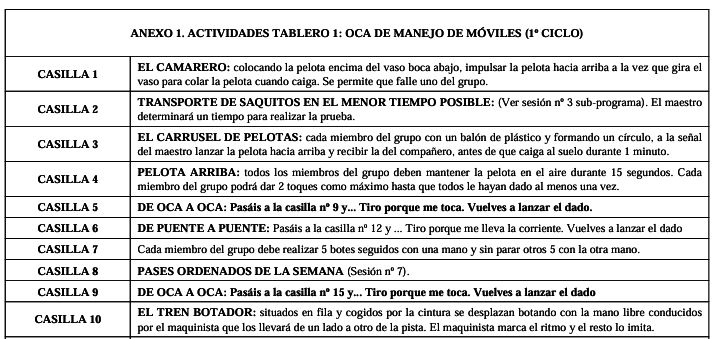
\includegraphics[width=1\textwidth]{imgs/casillas-oca-primaria.JPG}
	\caption{Diseño de la oca para evaluar las habilidades motoras en Educación Primaria \parencite{experienciaOca}}
	\label{fig:casillas-oca-primaria}
\end{figure}

\begin{figure}[h]
	\centering
	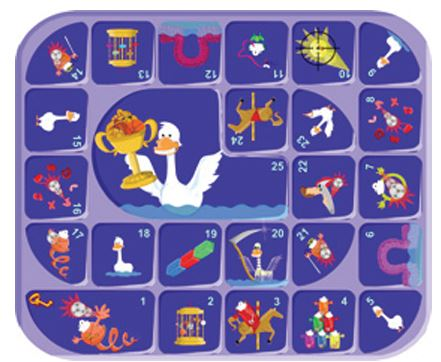
\includegraphics[width=0.45\textwidth]{imgs/oca-primaria.JPG}
	\caption{Tablero completo correspondiente a las casillas de la figura superior \parencite{experienciaOca}}
	\label{fig:oca-primaria}
\end{figure}


Esta medida tuvo gran éxito, pues los seguimientos del progreso de los participantes mostraron una mejoría general en sus destrezas físicas y capacidad de trabajo en equipo, así como una participación activa por parte de los estudiantes de Primaria que no se había registrado hasta el momento.

Por tanto, se ha querido replicar de alguna manera ese enfoque, trasladándolo a un contexto donde el grupo objetivo son los adultos mayores, y teniendo en cuenta la diversidad que puede existir dentro del mismo. 

Partiendo de la estructura del tablero original, hay una mayor probabilidad de que los adultos mayores estén familiarizados con su diseño y las reglas básicas, lo que puede contribuir a una experiencia de juego positiva y fluida.

\begin{figure}[H]
	\centering
	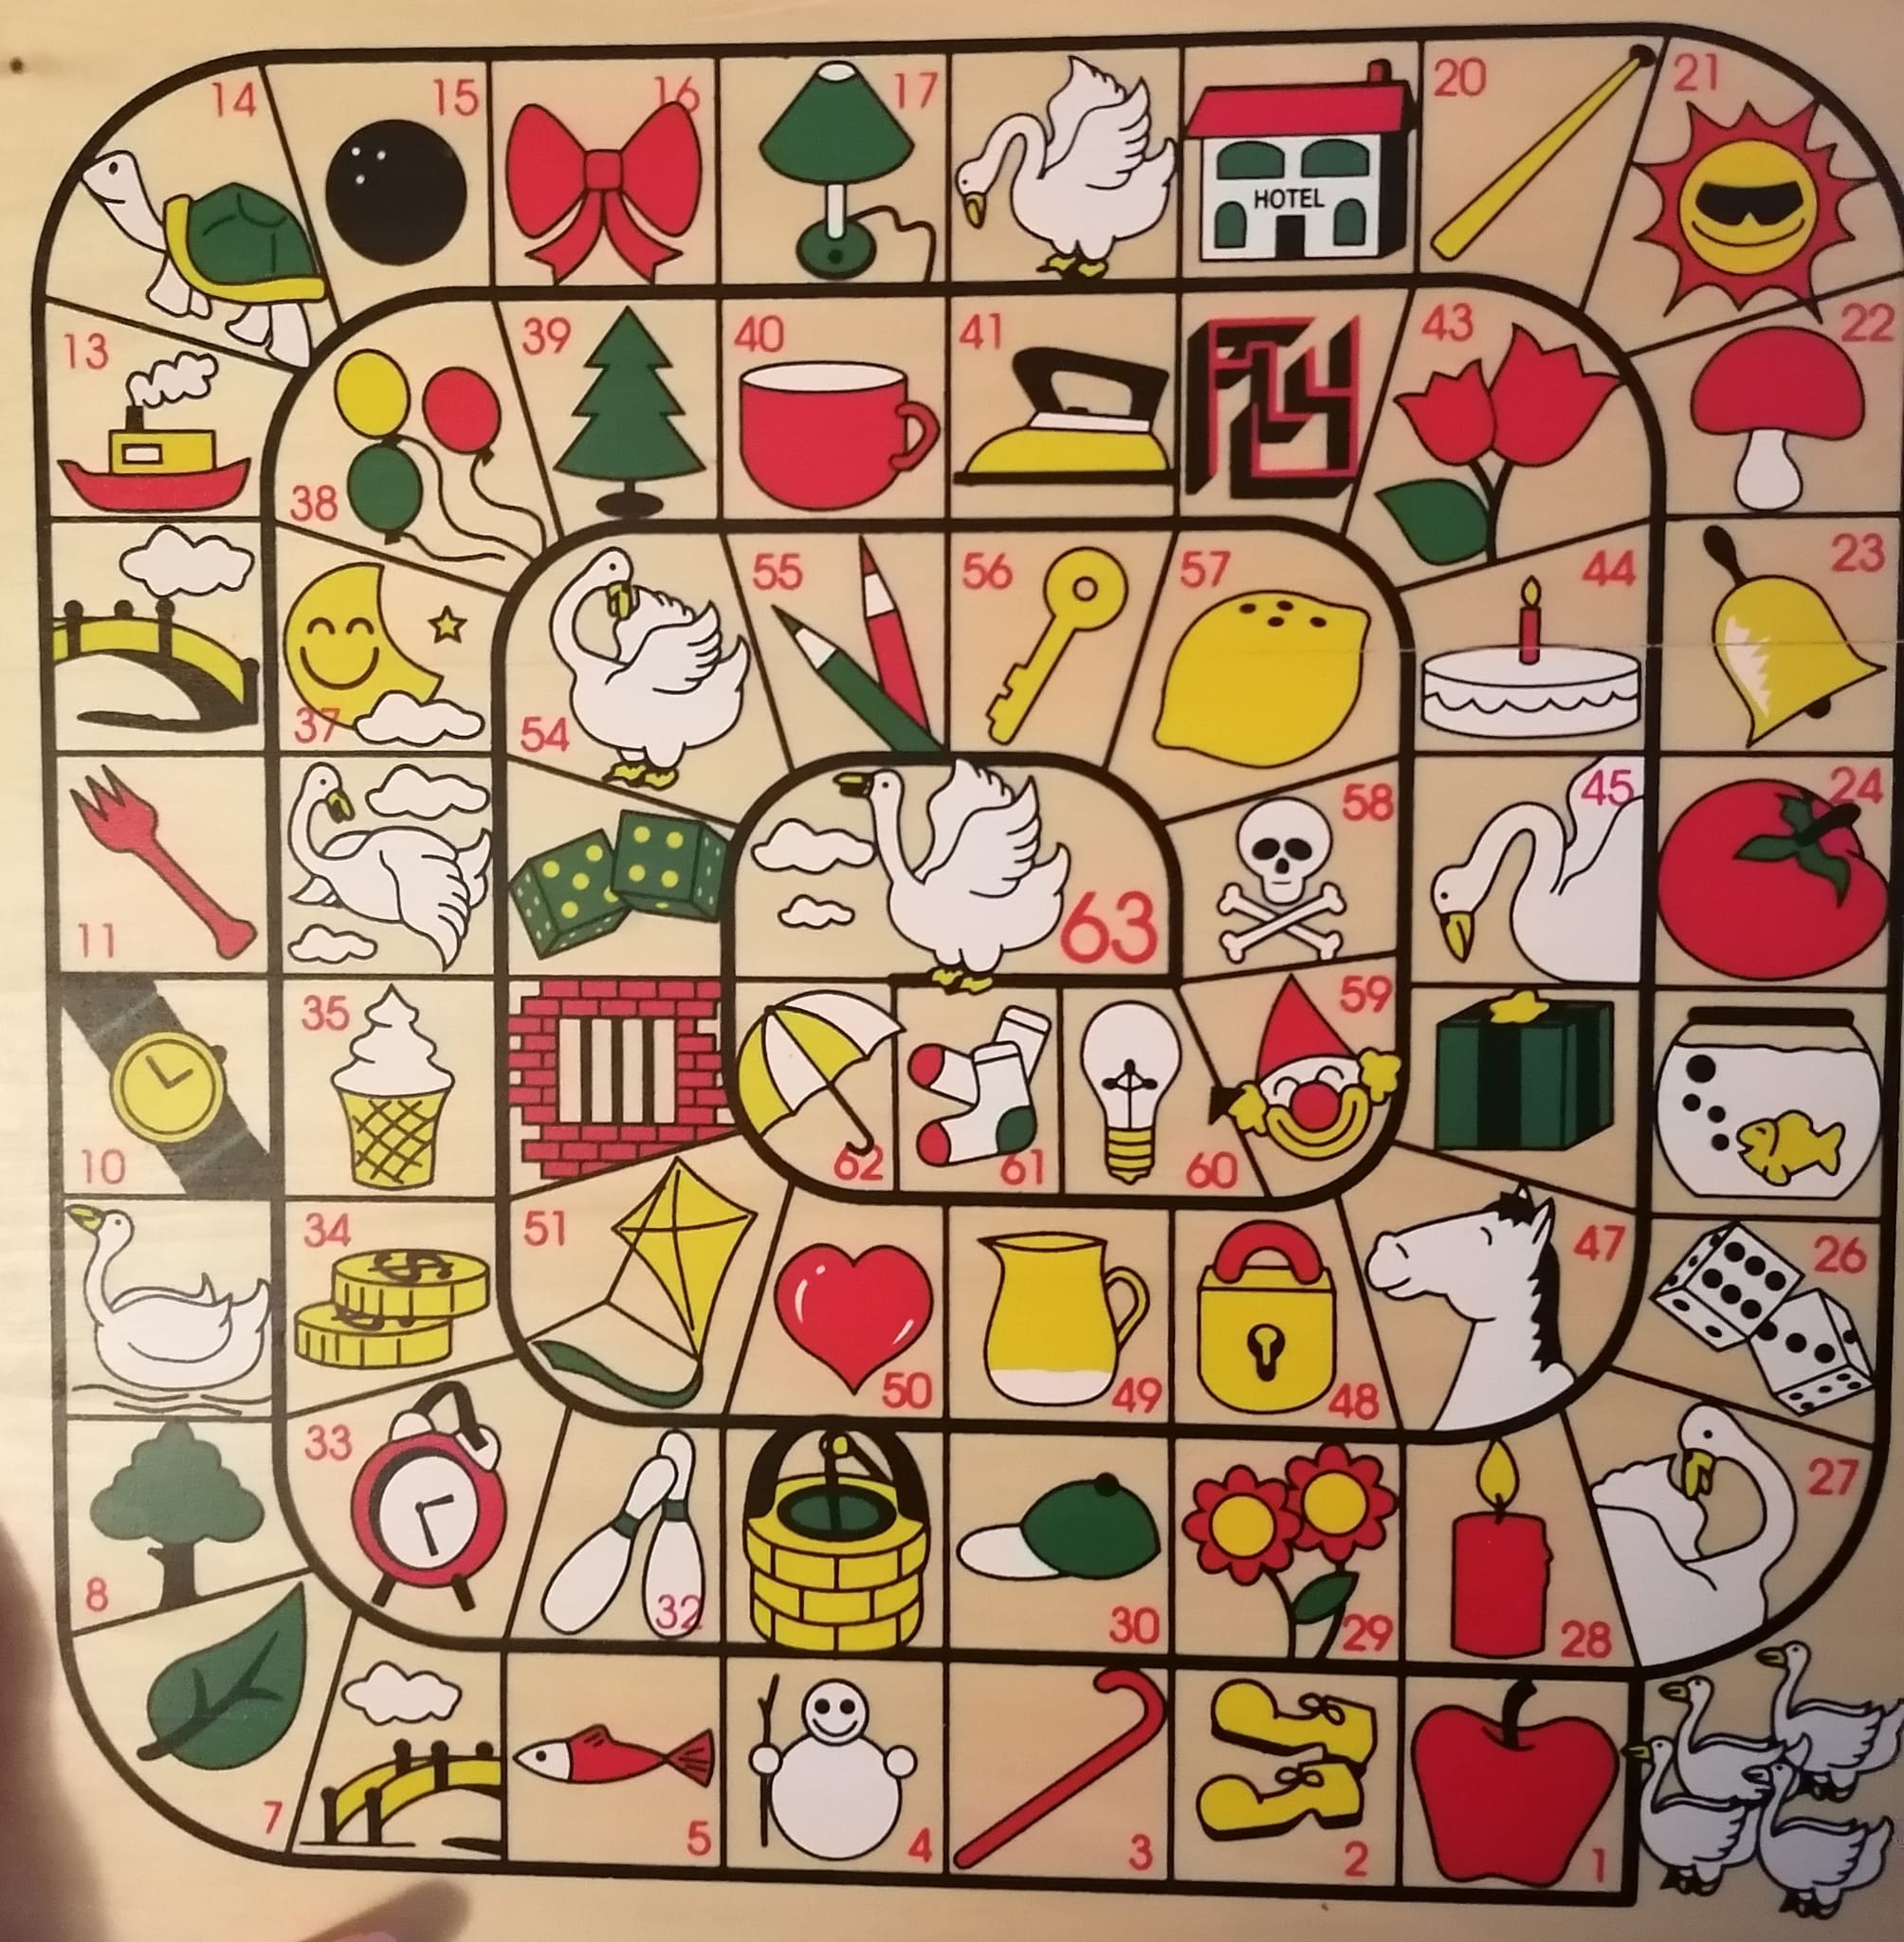
\includegraphics[width=0.7\textwidth]{imgs/oca-tradicional.jpg}
	\caption{Un tablero del juego tradicional de la oca}
	\label{fig:oca-tradicional}
\end{figure}


Sin embargo, al igual que la oca adaptada para estudiantes de Educación Primaria vista anteriormente, no se tratará de una oca tradicional cualquiera. 

Pues aparte de las casillas originales y el objetivo de llegar a la meta, incluirá un sistema de puntos, añadiendo un subobjetivo: el de conseguir la mayor puntuación antes de que termine la partida. Los participantes del juego podrán incrementar su marcador a través de una serie de minijuegos, que serán desencadenados cuando los jugadores caigan en determinadas casillas especiales.

También debe evaluarse la viabilidad de los minijuegos propuestos dentro del juego principal, que es la oca, para lo que se ha consultado con un equipo de psicólogos que han participado en varias experiencias de residencias.

\subsubsection{Lista de minijuegos dentro de la oca}
Dada la dificultad de implementar algunos en base a las limitaciones de los dispositivos Alexa, y para evitar saturar a los participantes con demasiadas mecánicas nuevas, se han elegido los siguientes cinco minijuegos:

\begin{enumerate}
	\item \textbf{Preguntas de Trivial V/F}: pondrán a prueba los conocimientos generales de los participantes. Se abordarán categorías distintas (geografía, historia, ciencia, arte y cultura…) pero siempre habrá dos opciones de respuesta, \textit{verdadero} o \textit{falso}. Si se acierta, se obtienen puntos, y si no, Alexa proporcionará una breve explicación de la respuesta correcta.
	\begin{itemize}
		\item Alexa: \textit{¿Oceanía es el continente más pequeño de todos?}
		\item Agustín: \textit{Verdadero.}
		\item Alexa: \textit{¡Correcto! Has ganado 10 puntos.}
		
		Alternativamente...
		\item Agustín: \textit{Falso.}
		\item Alexa: \textit{Incorrecto, el continente más pequeño del mundo es Oceanía, con 9.000.000 km² de superficie.}
	\end{itemize}
	
	\item \textbf{Conoce a tus compañeros}: Alexa planteará una pregunta acerca de otro participante, quien deberá colaborar, ya que luego tendrá que confirmar si la respuesta proporcionada por el primer participante es correcta o no. Siempre habrá dos tipos de respuestas, \textit{correcto/a} o \textit{incorrecto/a}.
	\begin{itemize}
		\item Alexa: \textit{Agustín, ¿Roberta ha viajado fuera del país alguna vez? Dime si es correcto o incorrecto.}
		\item Agustín: \textit{Correcto}
		\item Alexa: \textit{Roberta, ¿es esta respuesta correcta o incorrecta?}
		\item Roberta: \textit{Correcta}
		\item Alexa: \textit{¡Bien! Por conoceros tan bien, ambos ganáis puntos.}
	\end{itemize}
	
	\item \textbf{Adivina la cifra}: Alexa hará preguntas de todo tipo, cuya única respuesta es un número. Puede ser un año, la cantidad de algo... Es de modalidad competitiva, por lo que si el primero en responder la falla, la pregunta rebotará al siguiente, y así sucesivamente hasta que alguien acierte o se llegue de nuevo al primer participante, en cuyo caso Alexa desvelará la solución.
	\begin{itemize}
		\item Alexa: \textit{Agustín, ¿en qué año se descubrió América?}
		\item Agustín: \textit{1520}
		\item Alexa: \textit{Incorrecto, la pregunta rebota a Roberta. ¿En qué año se descubrió América?}
		\item Roberta: \textit{1492}
		\item Alexa: \textit{¡Correcto! Roberta gana 30 puntos.}
	\end{itemize}
	
	\item \textbf{Recuerda la última casilla}: Alexa preguntará por la casilla más reciente previa a la última tirada de dado; es decir, la casilla donde cayó en el turno anterior.
	\begin{itemize}
		\item Alexa: \textit{¿Cuál fue la última casilla en la que caíste en el turno anterior?}
		\item Roberta: \textit{La casilla del sombrero}
		\item Alexa: \textit{¡Correcto! Has ganado 'x' puntos.}
		
		Alternativamente...
		\item Roberta: \textit{Incorrecto, la respuesta correcta era: la casilla del paraguas.}
	\end{itemize}
	
	\item \textbf{Recuerda la fecha}: Alexa hará preguntas para poner a prueba la memoria de los participantes en relación con la orientación temporal, es decir, la forma en la que alguien mantiene la noción del tiempo. Las respuestas siempre serán días de la semana, meses o estaciones del año.
	\begin{itemize}
		\item Alexa: \textit{¿Qué día de la semana fue ayer?}
		\item Agustín: \textit{Jueves}
		...
		\item Alexa: \textit{¿En qué mes estamos?}
		\item Roberta: \textit{Julio}
	\end{itemize}
\end{enumerate}


\subsection{Historias de usuario y requisitos}

Las historias de usuario son imprescindibles en el desarrollo ágil de software, pero también resultan valiosas en cualquier otra metodología de desarrollo, ya sea tradicional o no. Pues a través de un formato sencillo, recogen de forma clara las necesidades y expectativas de los usuarios y clientes, facilitando la comunicación entre integrantes del equipo de desarrollo y clientes. Un ambiente colaborativo donde las ideas pueden fluctuar a medida que se avanza aumenta las probabilidades de éxito de cualquier proyecto \parencite{introHU}.

El formato típico de una historia de usuario se basa en los  tres elementos siguientes:

\begin{figure}[H]
	\centering
	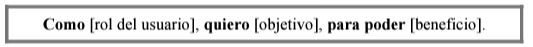
\includegraphics[width=0.88\textwidth]{imgs/formatoHU.jpg}
	\caption{Patrón general de una historia de usuario}
	\label{fig:formatoHU}
\end{figure}

Esta estructura facilita empatizar con la persona usuaria, entender qué pretende lograr sin entrar en detalles del "cómo" y el valor que aporta al producto, conocido como beneficio. Así, además de sintetizar en gran medida la información, permite cierta flexibilidad y la adaptación a cambios e integración de nuevas ideas durante el proceso de desarrollo.

Las historias de usuario ofrecen una perspectiva más centrada en los usuarios finales, mientras que los requisitos funcionales se limitan a describir el comportamiento del sistema. Entonces, merece la pena considerar ambos para que el producto final no solo cumpla con las especificaciones técnicas, sino que también otorgue valor real a quienes va dirigido.

\subsubsection{Historias de usuario}

Las siguientes historias de usuario establecen los requisitos de sistema del juego de la oca controlada por Alexa.

Estas contemplan desde la creación y configuración de una partida, hasta la gestión de turnos y control del estado del juego, garantizando asistencia activa durante todo el juego.

\begin{table}[H]
    \centering
    \begin{tabular}{|c|p{10cm}|}
        \hline
        \rowcolor{lightgray}
        \multicolumn{2}{|c|}{\textbf{HU01}: Iniciar el juego} \\
        \hline
        \textbf{Como} & jugador/a \\
        \hline
        \textbf{Quiero} & poder iniciar el juego de la oca \\
        \hline
        \textbf{Para} & empezar a jugar \\
        \hline
    \end{tabular}
    \caption{Historia de usuario nº 1}
    \label{tab:HU01}
\end{table}

\begin{table}[H]
	\centering
	\begin{tabular}{|c|p{10cm}|}
		\hline
		\rowcolor{lightgray}
		\multicolumn{2}{|c|}{\textbf{HU02}: Creación de una nueva partida} \\
		\hline
		\textbf{Como} & jugador/a \\
		\hline
		\textbf{Quiero} & poder iniciar un juego de la oca nuevo, pudiendo elegir cuántos jugadores van a participar, y si va ser por equipos o individualmente \\
		\hline
		\textbf{Para} & adaptar el juego a la cantidad y el tipo de participantes \\
		\hline
	\end{tabular}
	\caption{Historia de usuario nº 2}
	\label{tab:HU02}
\end{table}

\begin{table}[H]
    \centering
    \begin{tabular}{|c|p{10cm}|}
        \hline
        \rowcolor{lightgray}
        \multicolumn{2}{|c|}{\textbf{HU03}: Escuchar las reglas} \\
        \hline
        \textbf{Como} & jugador/a \\
        \hline
        \textbf{Quiero} & pedirle a Alexa que me explique las reglas y cualquier otro aspecto relevante del juego \\
        \hline
        \textbf{Para} & entender cómo jugar antes de comenzar o recordar alguna explicación durante la partida \\
        \hline
    \end{tabular}
    \caption{Historia de usuario nº 3}
    \label{tab:HU03}
\end{table}

\begin{table}[H]
    \centering
    \begin{tabular}{|c|p{10cm}|}
        \hline
        \rowcolor{lightgray}
        \multicolumn{2}{|c|}{\textbf{HU04}: Jugar un turno} \\
        \hline
        \textbf{Como} & jugador/a \\
        \hline
        \textbf{Quiero} & que Alexa tire los dados por mí y también mueva mi ficha \\
        \hline
        \textbf{Para} & jugar mi turno \\
        \hline
    \end{tabular}
    \caption{Historia de usuario nº 4}
    \label{tab:HU04}
\end{table}

\begin{table}[H]
    \centering
    \begin{tabular}{|c|p{10cm}|}
        \hline
        \rowcolor{lightgray}
        \multicolumn{2}{|c|}{\textbf{HU05}: Guardar la partida} \\
        \hline
        \textbf{Como} & jugador/a \\
        \hline
        \textbf{Quiero} & que Alexa tenga la capacidad de guardar el progreso de la partida actual \\
        \hline
        \textbf{Para} & poder retomar el juego más tarde sin perder el avance \\
        \hline
    \end{tabular}
    \caption{Historia de usuario nº 5}
    \label{tab:HU05}
\end{table}

\begin{table}[H]
    \centering
    \begin{tabular}{|c|p{10cm}|}
        \hline
        \rowcolor{lightgray}
        \multicolumn{2}{|c|}{\textbf{HU06}: Continuar la partida anterior} \\
        \hline
        \textbf{Como} & jugador/a \\
        \hline
        \textbf{Quiero} & poder continuar con la partida anterior si abro una nueva sesión \\
        \hline
        \textbf{Para} & reanudar la última partida donde la dejé \\
        \hline
    \end{tabular}
    \caption{Historia de usuario nº 6}
    \label{tab:HU06}
\end{table}

\begin{table}[H]
    \centering
    \begin{tabular}{|c|p{10cm}|}
        \hline
        \rowcolor{lightgray}
        \multicolumn{2}{|c|}{\textbf{HU07}: Recibir ayuda activa} \\
        \hline
        \textbf{Como} & jugador/a \\
        \hline
        \textbf{Quiero} & que Alexa me ofrezca ayuda activa durante el juego \\
        \hline
        \textbf{Para} & saber qué hacer por si me pierdo en cualquier momento \\
        \hline
    \end{tabular}
    \caption{Historia de usuario nº 7}
    \label{tab:HU07}
\end{table}

\begin{table}[H]
	\centering
	\begin{tabular}{|c|p{10cm}|}
		\hline
		\rowcolor{lightgray}
		\multicolumn{2}{|c|}{\textbf{HU08}: Finalizar el juego} \\
		\hline
		\textbf{Como} & jugador/a \\
		\hline
		\textbf{Quiero} & poder finalizar el juego en cualquier momento \\
		\hline
		\textbf{Para} & terminar la partida cuando lo desee \\
		\hline
	\end{tabular}
	\caption{Historia de usuario nº 8}
	\label{tab:HU08}
\end{table}

En el desarrollo del juego interactivo para Alexa, se han diseñado una serie de minijuegos que tienen como objetivo poner a prueba los conocimientos y la memoria de los participantes. Estos son los listados en la sección \textit{4.1.1}. 

A continuación, se presentan las historias de usuario para cada uno de estos minijuegos, que abarcan desde trivial de conocimiento general hasta desafíos de memoria y observación.

\begin{table}[H]
	\centering
	\begin{tabular}{|c|p{10cm}|}
		\hline
		\rowcolor{lightgray}
		\multicolumn{2}{|c|}{\textbf{HU09}: Minijuego verdadero o falso} \\
		\hline
		\textbf{Como} & jugador/a que ha caído en la casilla del minijuego de verdadero o falso \\
		\hline
		\textbf{Quiero} & responder a la pregunta planteada por Alexa con verdadero o falso y que me diga si he acertado \\
		\hline
		\textbf{Para} & poner a prueba mis conocimientos y ganar puntos \\
		\hline
	\end{tabular}
	\caption{Historia de usuario nº 9}
	\label{tab:HU09}
\end{table}

\begin{table}[H]
	\centering
	\begin{tabular}{|c|p{10cm}|}
		\hline
		\rowcolor{lightgray}
		\multicolumn{2}{|c|}{\textbf{HU10}: Minijuego conoce a tus compañeros} \\
		\hline
		\textbf{Como} & jugador/a que ha caído en la casilla del minijuego de conoce a tus compañeros \\
		\hline
		\textbf{Quiero} & responder a la pregunta acerca de otro jugador planteada por Alexa y que me confirmen si es correcto o no \\
		\hline
		\textbf{Para} & para demostrar cuánto conozco a mis compañeros y ganar puntos \\
		\hline
	\end{tabular}
	\caption{Historia de usuario nº 10}
	\label{tab:HU10}
\end{table}

\begin{table}[H]
	\centering
	\begin{tabular}{|c|p{10cm}|}
		\hline
		\rowcolor{lightgray}
		\multicolumn{2}{|c|}{\textbf{HU11}: Minijuego adivina la cifra} \\
		\hline
		\textbf{Como} & jugador/a en una ronda del minijuego de adivina la cifra \\
		\hline
		\textbf{Quiero} & responder a la preguntas planteada por Alexa con un número y que me diga si he acertado o no \\
		\hline
		\textbf{Para} & poner a prueba mis conocimientos y ganar puntos \\
		\hline
	\end{tabular}
	\caption{Historia de usuario nº 11}
	\label{tab:HU11}
\end{table}

\begin{table}[H]
	\centering
	\begin{tabular}{|c|p{10cm}|}
		\hline
		\rowcolor{lightgray}
		\multicolumn{2}{|c|}{\textbf{HU12}: Minijuego recuerda la última casilla} \\
		\hline
		\textbf{Como} & jugador/a que ha caído en la casilla del minijuego de recuerda la última casilla \\
		\hline
		\textbf{Quiero} & que responder con el nombre de la casilla en la que caí en el turno anterior \\
		\hline
		\textbf{Para} & poner a prueba mi memoria y ganar puntos \\
		\hline
	\end{tabular}
	\caption{Historia de usuario nº 12}
	\label{tab:HU12}
\end{table}

\begin{table}[H]
	\centering
	\begin{tabular}{|c|p{10cm}|}
		\hline
		\rowcolor{lightgray}
		\multicolumn{2}{|c|}{\textbf{HU13}: Minijuego recuerda la fecha} \\
		\hline
		\textbf{Como} & jugador/a que ha caído en la casilla del minijuego de recuerda la fecha \\
		\hline
		\textbf{Quiero} & responder a la pregunta planteada por Alexa con el nombre de un día de la semana, mes o estación del año  \\
		\hline
		\textbf{Para} & poner a prueba mi noción del tiempo y ganar puntos \\
		\hline
	\end{tabular}
	\caption{Historia de usuario nº 13}
	\label{tab:HU13}
\end{table}

\newpage
\subsubsection{Requisitos funcionales}

Esta sección define y describe las características de alto nivel (requisitos
funcionales) del sistema que son necesarias para cubrir las necesidades de los
usuarios. Se pueden estructurar de la siguiente manera:
\vspace{0.3cm}

\textbf{RF1: Iniciar la skill de Alexa}

Se debe poder lanzar la skill mediante el comando de invocación.
\vspace{0.5cm}

\textbf{RF2: Registro de datos de los participantes}
\begin{itemize}
	\item \textbf{RF2.1}: La skill debe preguntar el modo de juego: por equipos o jugadores individuales. 
	\item \textbf{RF2.2}: La skill debe preguntar el número de jugadores/equipos que van a participar.
	\item \textbf{RF2.3}: La skill debe registrar el nombre de los jugadores o equipos antes de empezar la partida.
\end{itemize}

\textbf{RF3: Simulación de un turno}
\begin{itemize}
    \item \textbf{RF3.1}: La skill debe incluir una función que simule el lanzamiento de dados y determine el número de casillas a avanzar.
    \item \textbf{RF3.2}: La skill debe incluir una función que mueva la ficha del jugador y muestre la casilla en la que ha caído.
\end{itemize}

\textbf{RF4: Gestión del estado del juego}
\begin{itemize}
    \item \textbf{RF4.1}: La skill debe ser capaz de guardar el estado actual del juego.
    \item \textbf{RF4.2}: Relacionado con el anterior, se debe poder reanudar la última partida con el estado con el que se ha guardado.
    \item \textbf{RF4.3}: Poder finalizar la partida en cualquier momento (borrando los datos del juego actual a no ser que se haya guardado previamente).
    \item \textbf{RF4.4}: Poder iniciar una nueva partida en cualquier momento (sobrescribiendo los datos guardados de la anterior).
\end{itemize}

\textbf{RF5: Explicación del juego}
\begin{itemize}
    \item \textbf{RF5.1}: Debe existir una opción dentro de la skill para explicar las reglas y objetivos del juego mediante un comando de voz.
    \item \textbf{RF5.2}: Debe existir una opción dentro de la skill para explicar los tipos de casillas del tablero mediante un comando de voz.
    \item \textbf{RF5.3}: Debe existir una opción dentro de la skill para explicar detalladamente los tipos de minijuegos mediante un comando de voz.
    \item \textbf{RF5.4}: Debe existir una opción dentro de la skill para que Alexa nombre y explique brevemente todos los comandos disponibles.
\end{itemize}

\textbf{RF6: Interacción continua}
\begin{itemize}
	\item \textbf{RF6.1}: La skill debe ser capaz de mantener una interacción continua con el usuario, a la espera de una respuesta en todo momento.
    \item \textbf{RF6.2}: La skill debe ofrecer asistencia en todo momento, en caso de que los participantes no sepan qué hacer a continuación y pase cierto tiempo sin recibir una respuesta, o que esta última no sea válida.
\end{itemize}

\textbf{RF7: Participar en un minijuego}
\begin{itemize}
	\item \textbf{RF7.1}: Cuando se cae en una casilla de minijuego, Alexa debe sacar un elemento aleatorio de la batería de preguntas correspondiente a dicho minijuego.
	\item \textbf{RF7.2}: La skill debe poder capturar la respuesta del participante y verificar si es correcta o no, actualizando sus puntos si es necesario.
\end{itemize}


\subsubsection{Requisitos no funcionales}

En este apartado se pueden ver las diferentes cualidades y restricciones del sistema (requisitos no funcionales) que no se relacionan de forma directa con el comportamiento del mismo.
\vspace{0.3cm}

\textbf{RNF1: Usabilidad}
\begin{itemize}
    \item \textbf{RNF1.1}: La skill debe ser fácil de usar y entender, especialmente diseñada para personas mayores.
    \item \textbf{RNF1.2}: Para evitar dudas, que Alexa explique de forma clara y fácil de entender lo que deben hacer los jugadores.
    \item \textbf{RNF1.3}: Alexa debe dejar un margen flexible de tiempo para esperar una respuesta y si no lo hace, repite la pregunta.
    \item \textbf{RNF1.4}: La interfaz debe ser simple y limitarse a mostrar los elementos relevantes de la partida para evitar saturar a los jugadores y jugadoras.
    \item \textbf{RNF1.5}: La fuente y disposición de elementos debe estar adaptada para la compresión y comodidad de los y las participantes.
\end{itemize}

\textbf{RNF2: Accesibilidad y compatibilidad}
\begin{itemize}
    \item \textbf{RNF2.1}: Es necesaria una cuenta de Amazon para instalar la skill y poder interactuar con Alexa.
    \item \textbf{RNF2.2}: Es necesario un dispositivo de Alexa con pantalla rectangular (como un Echo Show).
    \item \textbf{RNF2.3}: El dispositivo de Alexa debe tener una conexión estable a Internet.
    \item \textbf{RNF2.4}: La skill solo es compatible con el idioma español.
\end{itemize}

\textbf{RNF3: Rendimiento}
\begin{itemize}
    \item \textbf{RNF3.1}: Las respuestas a los comandos de voz deben ser rápidas, idealmente no superando los 5 segundos.
\end{itemize}

\textbf{RNF4: Fiabilidad}
\begin{itemize}
    \item \textbf{RNF4.1}: La skill debe funcionar correctamente en la mayoría de las interacciones, minimizando errores y malentendidos en el reconocimiento de voz.
\end{itemize}

\textbf{RNF5: Seguridad}
\begin{itemize}
	\item \textbf{RNF5.1}: Seguir las prácticas recomendadas basadas en principio de mínimo privilegio a la hora de utilizar los servicios de AWS.
\end{itemize}

\newpage
\subsection{Casos de uso y sus correspondientes diagramas}

Una vez se han detallado las historias y usuario y los requisitos del sistema, el siguiente paso es elaborar los casos de uso, asociados a los requisitos definidos previamente e incluso otros casos de uso. Esta técnica de ingeniería de software permite establecer la forma de interactuar entre los actores, entendidos como las entidades o sistema implicados en cada funcionalidad.  

\subsubsection{Casos de uso}

Como los actores siempre van a ser las personas usuarias y la asistente conversacional Alexa, se ha omitido esta fila en la plantilla de casos de uso, manteniendo únicamente en ella los aspectos fundamentales para comprender el curso normal de eventos y excepciones.

\begin{table}[H]
	\centering
	\begin{tabular}{|p{3cm}|p{12cm}|}
		\hline
		\rowcolor{lightgray}
		\multicolumn{2}{|c|}{\textbf{CU01}: Iniciar la skill} \\
		\hline
		\textbf{Descripción} & La persona usuaria interactúa con Alexa para abrir la skill \vspace{0.2cm} \\
		\hline
		\textbf{Precondiciones} & La skill está desplegada en la cuenta de Amazon vinculada al dispositivo Echo Show, que además debe tener acceso a Internet. \vspace{0.2cm} \\
		\hline
		\textbf{Postcondiciones} & El dispositivo muestra la pantalla de inicio \vspace{0.2cm} \\
		\hline
		\textbf{Referencias} & RF1 \vspace{0.2cm} \\
		\hline
		\textbf{Flujo normal de eventos} &
		\textbf{1.} La persona usuaria dice \enquote{Alexa, abre probando oca} para abrir la skill. \newline
		\vspace{0.2cm}
		\textbf{2.} Alexa realiza el lanzamiento de la skill, dando la bienvenida y una breve introducción al juego.
		\vspace{0.2cm} \\
		\hline
		\textbf{Flujo alterno de eventos} &
		\textbf{1.a.} Si la persona usuaria intenta jugar antes de haber lanzado la skill, Alexa dirá que no reconoce ninguno de los comandos. \vspace{0.2cm} \\
		\hline
	\end{tabular}
	\caption{Caso de uso nº 1}
	\label{tab:CU01}
\end{table}

\begin{table}[H]
	\centering
	\begin{tabular}{|p{3cm}|p{12cm}|}
		\hline
		\rowcolor{lightgray}
		\multicolumn{2}{|c|}{\textbf{CU02}: Pedir ayuda} \\
		\hline
		\textbf{Descripción} & La persona usuaria interactúa con Alexa para pedirle ayuda \vspace{0.2cm} \\
		\hline
		\textbf{Precondiciones} & La skill está iniciada. \vspace{0.2cm} \\
		\hline
		\textbf{Postcondiciones} & Alexa ofrece un listado de temas que puede explicar. \vspace{0.2cm} \\
		\hline
		\textbf{Referencias} & RF5.1, RF5.2, RF5.3 y RF5.4 \vspace{0.2cm} \\
		\hline
		\textbf{Flujo normal de eventos} &
		\textbf{1.} La persona usuaria dice \enquote{Ayuda} para que Alexa pueda asistirle. \newline
		\vspace{0.2cm}
		\textbf{2.} Alexa ofrece una lista de temas que puede explicar: las reglas y objetivos del juego, los tipos de casillas, los minijuegos y todos los comandos disponibles. Alexa dice que para aclarar uno de los temas, se debe decir \enquote{Explícame \textit{<tema>}}. \newline
		\vspace{0.2cm}
		\textbf{3.} La persona usuaria dice \enquote{Explícame \textit{<tema>}}, siendo \textit{<tema>} uno de los de la lista ofrecida por Alexa. \newline
		\vspace{0.2cm} 
		\textbf{4.} Alexa procede a explicar de forma clara el \textit{<tema>} preguntado por la persona usuaria.
		\vspace{0.2cm}\\
		\hline
		\textbf{Flujo alterno de eventos} &
		\textbf{3.a.} Si la persona usuaria intenta preguntar por un tema que no viene en la lista ofrecida por Alexa, repetirá la lista de temas que puede explicar. \vspace{0.2cm} \\
		\hline
	\end{tabular}
	\caption{Caso de uso nº 2}
	\label{tab:CU02}
\end{table}

\begin{table}[H]
	\centering
	\begin{tabular}{|p{3cm}|p{12cm}|}
		\hline
		\rowcolor{lightgray}
		\multicolumn{2}{|c|}{\textbf{CU03}: Crear una nueva partida} \\
		\hline
		\textbf{Descripción} & La persona usuaria interactúa con Alexa para crear una nueva partida del juego de la oca. \vspace{0.2cm} \\
		\hline
		\textbf{Precondiciones} & La skill está iniciada. \vspace{0.2cm} \\
		\hline
		\textbf{Postcondiciones} & Alexa crea una nueva partida con las configuraciones proporcionadas por la persona usuaria. \vspace{0.2cm} \\
		\hline
		\textbf{Referencias} & RF2.1, RF2.2, RF4.4, RF6.1 y RF6.2 \vspace{0.2cm} \\
		\hline
		\textbf{Flujo normal de eventos} &
		\textbf{1.} La persona usuaria le dice \enquote{Nueva partida} a Alexa. \newline
		\vspace{0.2cm}
		\textbf{2.} Alexa pregunta si los participantes van a jugar por equipos o individualmente. \newline
		\vspace{0.2cm}
		\textbf{3.} La persona usuaria responde: \enquote{por equipos} o \enquote{por jugadores individuales}. \newline
		\vspace{0.2cm} 
		\textbf{4.} Alexa pide confirmación, y después pregunta por el número de equipos/jugadores que van a participar en el juego. \newline
		\vspace{0.2cm}
		\textbf{5.} La persona usuaria responde con el número de participantes o equipos.\newline
		\vspace{0.2cm}
		\textbf{6.} Alexa confirma la respuesta, y después pide proceder con el registro de nombre de los equipos/participantes, dando instrucciones de cómo hacerlo.
		\vspace{0.2cm}\\
		\hline
		\textbf{Flujo alterno de eventos} &
		\textbf{3.a.} Si la persona usuaria dice un comando distinto a las dos posibles opciones, Alexa vuelve a preguntarle por el tipo de participantes. \vspace{0.2cm} \newline
		\textbf{5.a.} Si la persona usuaria responde con algo que no es un número, o es una cifra no válida (menor que 1 y mayor que 5), Alexa repite la pregunta del número de participantes. \vspace{0.2cm} \newline
		\textbf{4.a.} y \textbf{6.a.} Si la persona usuaria no le confirma su respuesta a Alexa, le volverá a formular la pregunta. \vspace{0.2cm}\\
		\hline
	\end{tabular}
	\caption{Caso de uso nº 3}
	\label{tab:CU03}
\end{table}

\begin{table}[H]
	\centering
	\begin{tabular}{|p{3cm}|p{12cm}|}
		\hline
		\rowcolor{lightgray}
		\multicolumn{2}{|c|}{\textbf{CU04}: Registro de participantes} \\
		\hline
		\textbf{Descripción} & Todos los equipos/participantes interactúan con Alexa para registrar sus nombres en el juego. \vspace{0.2cm} \\
		\hline
		\textbf{Precondiciones} & Se está creando una nueva partida y ya se han configurado los siguientes datos: tipo y número de participantes. \vspace{0.2cm} \\
		\hline
		\textbf{Postcondiciones} & Alexa anuncia el nombre de cada participante o equipo, muestra sus colores y nombres por pantalla, y anuncia el comienzo de la partida. \vspace{0.2cm} \\
		\hline
		\textbf{Referencias} & RF2.3, RF6.1 y RF6.2  |  CU03 \vspace{0.2cm} \\
		\hline
		\textbf{Flujo normal de eventos} &
		\textbf{1.} El primer equipo/participante dice \enquote{Nuestro/Mi nombre es \textit{<nombre}>} para que Alexa pueda registrarlo. \newline
		\vspace{0.2cm}
		\textbf{2.} Alexa confirma el nombre registrado y pide el del siguiente equipo/participante. \newline
		\vspace{0.2cm}
		\textbf{3.} El siguiente equipo/participante registra su nombre de la misma forma que el primero. \newline
		\vspace{0.2cm} 
		\textbf{4.} Alexa sigue pidiendo nombres hasta que se hayan registrado todos, en cuyo caso hace un resumen de los equipos/participantes registrados y los muestra por pantalla. Después hace una copia de los datos de la partida en la base de datos.
		\vspace{0.2cm}\\
		\hline
		\textbf{Flujo alterno de eventos} &
		\textbf{1.a.} y \textbf{3.a}. Si el equipo/participante no anuncia su nombre de la forma correcta establecida por Alexa, o Alexa no recibe respuesta en un rato, le recuerda que registre su nombre y cómo hacerlo. \vspace{0.2cm} \\
		\hline
	\end{tabular}
	\caption{Caso de uso nº 4}
	\label{tab:CU04}
\end{table}

\begin{table}[H]
	\centering
	\begin{tabular}{|p{3cm}|p{12cm}|}
		\hline
		\rowcolor{lightgray}
		\multicolumn{2}{|c|}{\textbf{CU05}: Jugar un turno} \\
		\hline
		\textbf{Descripción} & El equipo/participante actual juega su turno, compuesto por dos partes: tirar el dado y mover su ficha. \vspace{0.2cm} \\
		\hline
		\textbf{Precondiciones} & La partida ya está configurada y es el comienzo del turno del equipo/participante actual, quien no debe estar atrapado en alguna casilla de penalización. \vspace{0.2cm} \\
		\hline
		\textbf{Postcondiciones} & Alexa muestra por pantalla el color y nombre del equipo/participante actual y la casilla en la que ha caído, explicando el evento que esta ha desencadenado. \vspace{0.2cm} \\
		\hline
		\textbf{Referencias} & RF3.1, RF3.2, RF6.1 y RF6.2 \vspace{0.2cm} \\
		\hline
		\textbf{Flujo normal de eventos} &
		\textbf{1.} El equipo/participante actual dice \enquote{Tirar dado}. \newline
		\vspace{0.2cm}
		\textbf{2.} Alexa muestra la tira de dado por pantalla y anuncia el número del 1 al 6 que ha salido. Después le indica que mueva su ficha. \newline
		\vspace{0.2cm}
		\textbf{3.} El equipo/participante actual dice \enquote{Mover ficha}. \newline
		\vspace{0.2cm} 
		\textbf{4.} Alexa informa sobre su movimiento, mostrando por pantalla el nombre y color del equipo/participante actual, así como en la casilla que ha caído. Alexa la describe y da las instrucciones adicionales necesarias en caso de ser una casilla especial.
		\vspace{0.2cm}\\
		\hline
		\textbf{Flujo alterno de eventos} &
		\textbf{1.a.} y \textbf{3.a}. Si el equipo/participante actual dice un comando no accesible en ese momento o distinto al especificado, Alexa le repetirá lo que debe decir para avanzar en el juego. \vspace{0.2cm} \\
		\hline
	\end{tabular}
	\caption{Caso de uso nº 5}
	\label{tab:CU05}
\end{table}

\begin{table}[H]
	\centering
	\begin{tabular}{|p{3cm}|p{12cm}|}
		\hline
		\rowcolor{lightgray}
		\multicolumn{2}{|c|}{\textbf{CU06}: Guardar la partida} \\
		\hline
		\textbf{Descripción} & La persona usuaria guarda el estado de la partida actual para que persista de una sesión a otra. \vspace{0.2cm} \\
		\hline
		\textbf{Precondiciones} & La partida actual ya está configurada, y solo puede guardarse al comienzo de turno de cualquier jugador, es decir, antes de tirar el dado. \vspace{0.2cm} \\
		\hline
		\textbf{Postcondiciones} & Alexa anuncia que se han guardado los datos correctamente, al haber sido enviados con éxito a la base de datos. \vspace{0.2cm} \\
		\hline
		\textbf{Referencias} & RF4.1 \vspace{0.2cm} \\
		\hline
		\textbf{Flujo normal de eventos} &
		\textbf{1.} La persona usuaria dice \enquote{Guardar partida}. \newline
		\vspace{0.2cm}
		\textbf{2.} Alexa envía los datos de la partida y de los jugadores a la base de datos de DynamoDB y anuncia que la operación tuvo éxito.
		\vspace{0.2cm}\\
		\hline
		\textbf{Flujo alterno de eventos} &
		\textbf{1.a.} No dejará guardar la partida si se encuentra en mitad de un turno (moviendo la ficha o participando en un minijuego). \vspace{0.2cm} \\
		\hline
	\end{tabular}
	\caption{Caso de uso nº 6}
	\label{tab:CU06}
\end{table}

\begin{table}[H]
	\centering
	\begin{tabular}{|p{3cm}|p{12cm}|}
		\hline
		\rowcolor{lightgray}
		\multicolumn{2}{|c|}{\textbf{CU07}: Continuar la partida} \\
		\hline
		\textbf{Descripción} & La persona usuaria le indica que cargue los datos de la anterior partida que fueron guardados en la base de datos. \vspace{0.2cm} \\
		\hline
		\textbf{Precondiciones} & Tiene que haber una partida guardada de sesiones anteriores \vspace{0.2cm} \\
		\hline
		\textbf{Postcondiciones} & Se carga los datos de la última partida guardada y se retoma el juego desde el punto en el que se dejó. \vspace{0.2cm} \\
		\hline
		\textbf{Referencias} & RF4.2 \vspace{0.2cm} \\
		\hline
		\textbf{Flujo normal de eventos} &
		\textbf{1.} La persona usuaria dice \enquote{Continuar última partida}. \newline
		\vspace{0.2cm}
		\textbf{2.} Alexa carga los datos de la partida guardada en sesiones anteriores y recuerda el turno en el que se quedó el juego.
		\vspace{0.2cm}\\
		\hline
		\textbf{Flujo alterno de eventos} &
		\textbf{1.a.} Si no hay datos guardados, no podrá cargarlos y habrá que crear una partida nueva. \vspace{0.2cm} \\
		\hline
	\end{tabular}
	\caption{Caso de uso nº 7}
	\label{tab:CU07}
\end{table}


\begin{table}[H]
	\centering
	\begin{tabular}{|p{3cm}|p{12cm}|}
		\hline
		\rowcolor{lightgray}
		\multicolumn{2}{|c|}{\textbf{CU08}: Minijuego verdadero o falso} \\
		\hline
		\textbf{Descripción} & El equipo/participante actual participa en el minijuego de verdadero o falso para la posibilidad de ganar 10 puntos. \vspace{0.2cm} \\
		\hline
		\textbf{Precondiciones} & El equipo/participante actual ha caído en una casilla del minijuego verdadero o falso. \vspace{0.2cm} \\
		\hline
		\textbf{Postcondiciones} & Se actualizan los puntos del equipo/participante actual si es necesario, y se anuncia el siguiente turno. \vspace{0.2cm} \\
		\hline
		\textbf{Referencias} & RF6.1, RF6.2, RF7.1 y RF7.2 \vspace{0.2cm} \\
		\hline
		\textbf{Flujo normal de eventos} &
		\textbf{1.} Alexa le hace una pregunta de trivial de verdadero o falso al equipo/participante actual. \newline
		\vspace{0.2cm}
		\textbf{2.} El equipo/participante actual responde con \enquote{verdadero} o \enquote{falso}. \newline
		\vspace{0.2cm}
		\textbf{3.} Alexa verifica si su respuesta es correcta o no, actualizando sus puntos en caso afirmativo, o dando una breve explicación de la respuesta correcta en caso contrario. \newline
		\vspace{0.2cm} \\
		\hline
		\textbf{Flujo alterno de eventos} &
		\textbf{2.a.} Si la respuesta proporcionada no es del tipo verdadero o falso, Alexa repetirá la pregunta, aclarando el formato de respuesta que debe dar. \newline
		\vspace{0.2cm} 
		\textbf{2.b.} Si Alexa no recibe una respuesta válida en un rato, repetirá la pregunta, aclarando el tipo de respuesta que debe dar. \vspace{0.2cm} \\
		\hline
	\end{tabular}
	\caption{Caso de uso nº 8}
	\label{tab:CU08}
\end{table}

\begin{table}[H]
	\centering
	\begin{tabular}{|p{3cm}|p{12cm}|}
		\hline
		\rowcolor{lightgray}
		\multicolumn{2}{|c|}{\textbf{CU09}: Minijuego conoce a tus compañeros} \\
		\hline
		\textbf{Descripción} & El equipo/participante actual participa en el minijuego de conoce a tus compañeros para la posibilidad de ganar 15 puntos. \vspace{0.2cm} \\
		\hline
		\textbf{Precondiciones} & El equipo/participante actual ha caído en una casilla del minijuego conoce a tus compañeros. \vspace{0.2cm} \\
		\hline
		\textbf{Postcondiciones} & Se actualizan los puntos de los equipos/participantes involucrados si es necesario, y se anuncia el siguiente turno. \vspace{0.2cm} \\
		\hline
		\textbf{Referencias} & RF6.1, RF6.2, RF7.1 y RF7.2 \vspace{0.2cm} \\
		\hline
		\textbf{Flujo normal de eventos} &
		\textbf{1.} Alexa le hace una pregunta al equipo/participante actual, acerca de otro equipo/participante aleatorio. \newline
		\vspace{0.2cm}
		\textbf{2.} El equipo/participante actual responde con \enquote{correcto/a} o \enquote{incorrecto/a}. \newline
		\vspace{0.2cm}
		\textbf{3.} Alexa le pide al equipo/participante sobre el que iba la pregunta que confirme si la respuesta dada es correcta o incorrecta. \newline
		\vspace{0.2cm} 
		\textbf{4.} El sujeto de la pregunta confirma si es correcta o incorrecta la respuesta del equipo/participante actual. \newline
		\vspace{0.2cm} 
		\textbf{5.} Si es correcta, Alexa otorga puntos a ambas partes implicadas y pasa al siguiente turno. Si ha fallado, pasa de turno directamente.
		\vspace{0.2cm} \\
		\hline
		\textbf{Flujo alterno de eventos} &
		\textbf{2.a.} Si la respuesta proporcionada no es del tipo correcto/a o incorrecto/a, Alexa repetirá la pregunta, aclarando el formato de respuesta que debe dar. \newline
		\vspace{0.2cm} 
		\textbf{2.b.} Si Alexa no recibe una respuesta válida en un rato, repetirá la pregunta, aclarando el tipo de respuesta que debe dar. \vspace{0.2cm} \\
		\hline
	\end{tabular}
	\caption{Caso de uso nº 9}
	\label{tab:CU09}
\end{table}

\begin{table}[H]
	\centering
	\begin{tabular}{|p{3cm}|p{12cm}|}
		\hline
		\rowcolor{lightgray}
		\multicolumn{2}{|c|}{\textbf{CU10}: Minijuego adivina la cifra} \\
		\hline
		\textbf{Descripción} & El equipo/participante actual participa en el minijuego de conoce a adivina la cifra para la posibilidad de ganar 30 puntos. \vspace{0.2cm} \\
		\hline
		\textbf{Precondiciones} & El equipo/participante actual ha caído en una casilla del minijuego adivina la cifra. \vspace{0.2cm} \\
		\hline
		\textbf{Postcondiciones} & Se actualizan los puntos del equipo/participante que ha acertado si es necesario, y se anuncia el siguiente turno. \vspace{0.2cm} \\
		\hline
		\textbf{Referencias} & RF6.1, RF6.2, RF7.1 y RF7.2 \vspace{0.2cm} \\
		\hline
		\textbf{Flujo normal de eventos} &
		\textbf{1.} Alexa le hace una pregunta al equipo/participante actual, cuya respuesta debe ser únicamente un número. \newline
		\vspace{0.2cm}
		\textbf{2.} El equipo/participante actual responde con una cifra. \newline
		\vspace{0.2cm}
		\textbf{3.} Alexa verifica si es correcta, dándole puntos en caso afirmativo. En caso de fallo, repetirá la pregunta al siguiente equipo/participante. \newline
		\vspace{0.2cm} 
		\textbf{4.} El siguiente responde con una cifra distinta que piense que pueda ser la correcta. \newline
		\vspace{0.2cm} 
		\textbf{5.} Alexa continúa preguntando al siguiente, así hasta que alguien acierte o se haya dado una vuelta completa por todos los equipos/participantes, en cuyo caso desvelará la solución.
		\vspace{0.2cm} \\
		\hline
		\textbf{Flujo alterno de eventos} &
		\textbf{2.a.} y \textbf{4.a.} Si la respuesta proporcionada no es un número, Alexa repetirá la pregunta, aclarando el formato de respuesta que debe dar. \newline
		\vspace{0.2cm} 
		\textbf{2.b.} y \textbf{4.a.} Si Alexa no recibe una respuesta válida en un rato, repetirá la pregunta, aclarando el tipo de respuesta que debe dar. \vspace{0.2cm} \\
		\hline
	\end{tabular}
	\caption{Caso de uso nº 10}
	\label{tab:CU10}
\end{table}

\begin{table}[H]
	\centering
	\begin{tabular}{|p{3cm}|p{12cm}|}
		\hline
		\rowcolor{lightgray}
		\multicolumn{2}{|c|}{\textbf{CU11}: Minijuego recuerda la última casilla} \\
		\hline
		\textbf{Descripción} & El equipo/participante actual participa en el minijuego de recuerda la última casilla para la posibilidad de ganar 25 puntos. \vspace{0.2cm} \\
		\hline
		\textbf{Precondiciones} & El equipo/participante actual ha caído en una casilla de recuerda la última casilla. \vspace{0.2cm} \\
		\hline
		\textbf{Postcondiciones} & Se actualizan los puntos del equipo/participante actual si es necesario, y se anuncia el siguiente turno. \vspace{0.2cm} \\
		\hline
		\textbf{Referencias} & RF6.1, RF6.2, RF7.1 y RF7.2 \vspace{0.2cm} \\
		\hline
		\textbf{Flujo normal de eventos} &
		\textbf{1.} Alexa le pregunta al equipo/participante actual el nombre de la última casilla en la que estaba, previa a la actual. \newline
		\vspace{0.2cm}
		\textbf{2.} El equipo/participante actual responde con el nombre de la casilla en la que piensa que estaba en el turno anterior. \newline
		\vspace{0.2cm}
		\textbf{3.} Alexa verifica si su respuesta es correcta o no, actualizando sus puntos en caso afirmativo, o desvelando el nombre de la casilla correcta en caso contrario. \newline
		\vspace{0.2cm} \\
		\hline
		\textbf{Flujo alterno de eventos} &
		\textbf{2.a.} Si la respuesta proporcionada no es un nombre de casilla válido, Alexa repetirá la pregunta, aclarando el formato de respuesta que debe dar. \newline
		\vspace{0.2cm} 
		\textbf{2.b.} Si Alexa no recibe una respuesta válida en un rato, repetirá la pregunta, aclarando el tipo de respuesta que debe dar. Si no recuerda ningún nombre de casilla, le indica que diga \enquote{No me acuerdo de la casilla} para pasar de turno.
		\vspace{0.2cm} \\
		\hline
	\end{tabular}
	\caption{Caso de uso nº 11}
	\label{tab:CU11}
\end{table}

\begin{table}[H]
	\centering
	\begin{tabular}{|p{3cm}|p{12cm}|}
		\hline
		\rowcolor{lightgray}
		\multicolumn{2}{|c|}{\textbf{CU12}: Minijuego recuerda la fecha} \\
		\hline
		\textbf{Descripción} & El equipo/participante actual participa en el minijuego de recuerda la fecha para la posibilidad de ganar 20 puntos. \vspace{0.2cm} \\
		\hline
		\textbf{Precondiciones} & El equipo/participante actual ha caído en una casilla de recuerda la fecha. \vspace{0.2cm} \\
		\hline
		\textbf{Postcondiciones} & Se actualizan los puntos del equipo/participante actual si es necesario, y se anuncia el siguiente turno. \vspace{0.2cm} \\
		\hline
		\textbf{Referencias} & RF6.1, RF6.2, RF7.1 y RF7.2 \vspace{0.2cm} \\
		\hline
		\textbf{Flujo normal de eventos} &
		\textbf{1.} Alexa le hace una pregunta sobre un día de la semana, mes o estación del año concreto. \newline
		\vspace{0.2cm}
		\textbf{2.} El equipo/participante actual responde con el nombre del día de la semana, mes o estación del año que piense que es la correcta. \newline
		\vspace{0.2cm}
		\textbf{3.} Alexa verifica si se ha acordado bien o no, actualizando sus puntos en caso afirmativo, o recordando la solución en caso contrario. \newline
		\vspace{0.2cm} \\
		\hline
		\textbf{Flujo alterno de eventos} &
		\textbf{2.a.} Si la respuesta proporcionada no es un día de la semana, mes o estación del año, Alexa repetirá la pregunta, aclarando el formato de respuesta que debe dar. \newline
		\vspace{0.2cm} 
		\textbf{2.b.} Si Alexa no recibe una respuesta válida en un rato, repetirá la pregunta, aclarando el tipo de respuesta que debe dar.
		\vspace{0.2cm} \\
		\hline
	\end{tabular}
	\caption{Caso de uso nº 12}
	\label{tab:CU12}
\end{table}

\begin{table}[H]
	\centering
	\begin{tabular}{|p{3cm}|p{12cm}|}
		\hline
		\rowcolor{lightgray}
		\multicolumn{2}{|c|}{\textbf{CU13}: Cerrar la skill} \\
		\hline
		\textbf{Descripción} & La persona usuaria interactúa con Alexa para cerrar la skill \vspace{0.2cm} \\
		\hline
		\textbf{Precondiciones} & La skill está iniciada. \vspace{0.2cm} \\
		\hline
		\textbf{Postcondiciones} & Se cierra la skill del juego de la oca, borrando los datos de la partida actual a no ser que se hayan guardado en la base de datos antes. \vspace{0.2cm} \\
		\hline
		\textbf{Referencias} & RF4.3 \vspace{0.2cm} \\
		\hline
		\textbf{Flujo normal de eventos} &
		\textbf{1.} La persona usuaria dice \enquote{Cierra probando oca} para cerrar la skill. \newline
		\vspace{0.2cm}
		\textbf{2.} Alexa manda la orden de terminar la sesión, marcando el fin de la partida y cerrando la skill.
		\vspace{0.2cm} \\
		\hline
		\textbf{Flujo alterno de eventos} &
		\textbf{2.a.} Si la persona usuaria intenta jugar después de haber cerrado la skill, Alexa dirá que no reconoce ninguno de los comandos y habrá que abrir la skill de nuevo. \vspace{0.2cm} \\
		\hline
	\end{tabular}
	\caption{Caso de uso nº 13}
	\label{tab:CU13}
\end{table}

\newpage
\subsubsection{Matriz de cobertura de requisitos funcionales}

A continuación, se comprueba que todos los casos de uso definidos en la sección anterior referencian a un requisitos funcionales como mínimo. 

Dicho de otra forma, todos los requisitos funcionales deben estar cubiertos por al menos un caso de uso.

\begin{figure}[H]
	\centering
	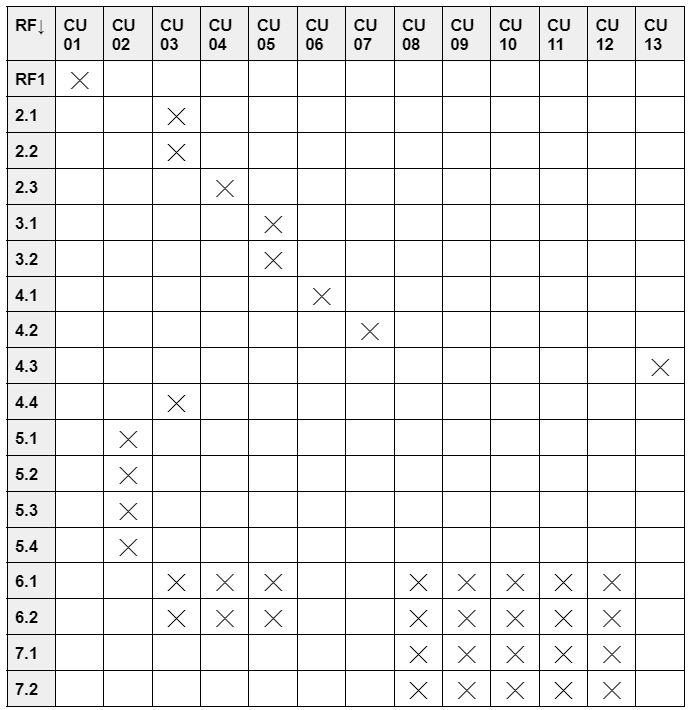
\includegraphics{imgs/matriz-requisitos.JPG}
	\caption{Matriz de cobertura de requisitos funcionales}
	\label{fig:matriz-requisitos}
\end{figure}

\subsubsection{Diagramas de secuencia}





\newpage
\input{secciones/5_diseño}

\newpage
\section{Análisis tecnológico}

En esta sección se van a examinar algunas de las herramientas y conocimentos tecnológicos necesarios para el desarrollo posterior de la skill, de los que se ha podido generar una idea clara con el apoyo de la documentación oficial de Alexa \parencite{alexaDocs}.

\subsection{Fundamentos de una skill}

Familiarizarse con los fundamentos de una skill implica comprender los conceptos clave usados en el contexto de una interacción entre una persona usuaria y Alexa, así como el funcionamiento general de la persistencia de datos dentro del código de la skill.

\subsubsection{Términos comunes en el desarrollo de skills}

Para comprender mejor la terminología en la documentación de este proyecto, se explican los conceptos siguientes:

\begin{itemize}
	\item \textit{\textbf{Intents}}: representan las intenciones de las personas usuarias, entendidas como las acciones llevadas a cabo con una finalidad, las cuales son llamadas a través determinadas frases. Por ejemplo, el intent \textit{guardarPartidaIntent} cumple con el objetivo de guardar el estado de la partida.
	\item \textit{\textbf{Utterances}}: son precisamente las frases de activación que se mencionaban antes. Explicado de otra forma, serían los comandos de voz que pueden utilizarse para invocar intents específicos, por lo que deben ser frases intuitivas y que difieran entre sí. Siguiendo el caso anterior, si se quiere llamar a \textit{guardarPartidaIntent}, las utterances podrían ser <<guarda mi partida>>, <<guárdame la partida>>, etc.
	\item \textit{\textbf{Handlers}}: son funciones encargadas de implementar la lógica de una skill. Están asociados a un intent para ejecutar el código que procese la respuesta esperada de dicho intent. Por ejemplo, el manejador \textit{guardarPartidaHandler}, que encapsula la lógica necesaria para el intent de ejemplo.
	\item \textit{\textbf{Slots}}: los intents pueden tener definidos slots de manera opcional. Se podrían describir como argumentos que Alexa captura de una determinada solicitud o respuesta de la persona usuaria, y que permiten guardar valores concretos para completar la lógica de los manejadores. Un ejemplo es si se tiene un intent, \textit{crearJugadoresIntent}, que cualquier usuario/a puede invocar diciendo <<Crea [tres] jugadores>>. Tres es capturado por el slot configurado para guardar el número de jugadores a crear.
\end{itemize}

\subsubsection{Memoria y persistencia de datos}

Entender cómo funciona la persistencia de datos en las skills es esencial para saber cómo abordar su desarrollo y garantizar que se mantiene un contexto adecuado durante toda la interacción con Alexa.

Se distinguen los dos mecanismos principales para la memoria de datos en skills que serán considerados para este proyecto: los atributos de sesión (\textit{session attributes}) y las bases de datos.

Los atributos de sesión, como da a entender el nombre, se ubican en el contexto de la sesión activa actual. Resultan útiles cuando se quiere mantener cierta información de un handler a otro, pero de manera temporal.

A continuación, se muestran los métodos básicos de consulta (o acceso) y modificación de un atributo de sesión, facilitados por la clase gestora de atributos que proporciona el SDK de Alexa (biblioteca específica de ASK, ver sección \textit{6.2.}).

\begin{figure}[H]
	\centering
	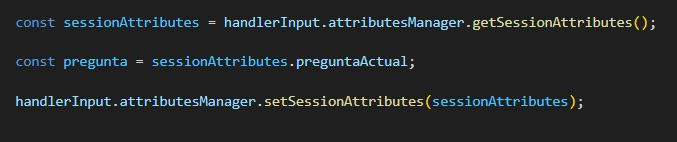
\includegraphics[width=0.93\textwidth]{imgs/sesion-atrib.jpg}
	\caption{Métodos básicos del gestor de atributos}
	\label{fig:sesion-atrib}
\end{figure}

Por otro lado, las bases de datos se diferencian en que sí permiten mantener información entre sesiones, de forma escalable y a largo plazo. Es la alternativa a tomar si se manejan estructuras de datos más complejas y/o necesarias en el contexto de futuras interacciones.

Las bases de dato pueden ser relacionales o no, aunque para las skills de Alexa es común optar por la opción NoSQL de \textit{DynamoDB}, puesto que es un servicio que ya viene integrado en AWS (ver sección \textit{6.3.}), adecuado gracias a su alta disponibilidad y buen rendimiento.

\subsection{Alexa Skills Kit (ASK)}

ASK es un conjunto de APIs y herramientas que facilitan la integración de nuevas habilidades en Alexa, permitiendo crear distintas clases de skills, desde personalizadas hasta otras específicas para vídeo, listas y hogar inteligente.

El tipo de skill que mejor se ajusta a los objetivos preestablecidos es la personalizada o \textit{Custom Skill}, pues esta permite más flexibilidad a los desarrolladores, permitiéndoles adaptarla a las necesidades de la aplicación a desarrollar.

Se puede importar ASK, a través del nombre de la biblioteca: \textit{ask-sdk-core}.

\subsection{AWS Serverless Platform}

Para el desarrollo de skills de Alexa, se puede optar o bien por la función Lambda de AWS, o bien por un servicio web distinto. La primera opción pertenece a un conjunto de herramientas de desarrollador y servicios en la nube de alto rendimiento que componen la Plataforma sin Servidor de AWS.

Se va a utilizar \textbf{AWS Lambda} para la creación de este juego digital, aprovechando así las múltiples funcionalidades y material de apoyo para encaminar el proceso de desarrollo. Además, al poder hacer uso de los otros servicios incluidos en esta plataforma (DynamoDB, Amazon S3, etc), se garantiza cierta centralización y absoluta compatibilidad entre ellos.

\subsection{Alexa Presentation Language (APL)}

La parte visual de la skill se gestiona mediante el lenguaje de presentación de Alexa (APL), a través del envío de documentos APL al dispositivo en forma de una directiva que se verá más adelante.

Un documento APL consiste en un fichero JSON que define la estructura y disposición de elementos a mostrar por la pantalla del dispositivo de Alexa.
A continuación se muestra un ejemplo básico de documento APL que imprime por pantalla una cadena de texto:

\begin{figure}[H]
	\centering
	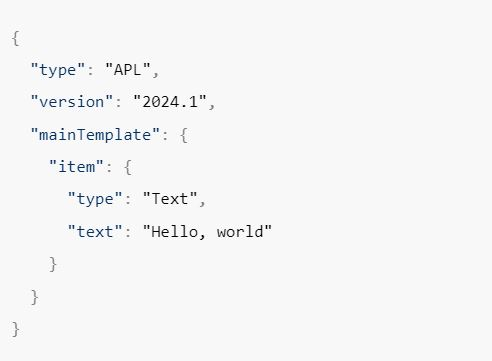
\includegraphics[width=0.6\textwidth]{imgs/apl-example.JPG}
	\caption{Ejemplo de documento APL básico (\href{https://developer.amazon.com/en-US/docs/alexa/alexa-presentation-language/apl-document.html}{Alexa Developer Documentation})}
	\label{fig:apl-ejemplo}
\end{figure}



\newpage
\section{Desarrollo}

Una vez pasada a la fase de desarrollo, el objetivo es transformar el diseño y requisitos concretados previamente en una aplicación funcional. 

Este proceso implica la creación de la skill, el desarrollo de código y la realización de pruebas, pero no sin antes haber cumplido dos prerrequisitos:
\begin{itemize}
	\item Tener una cuenta en \textit{Alexa developer console}, que es de carácter totalmente gratuito y permitirá el alojamiento y despliegue de la skill. 
	\item Tener una cuenta de \textit{Amazon Web Services} (AWS), para lo que se debe ingresar un método de pago. Esto es necesario en caso de que el uso de recursos exceda los límites de la oferta gratuita y Amazon tenga que cobrar una cantidad adicional.
\end{itemize}

\subsection{Creación de la skill y el modelo de interacción}

Hay una gran cantidad de guías disponibles para aprender a crear una skill desde cero, y la propia página oficial de desarrolladores Alexa \parencite{alexaHosted} ofrece diversos documentos de apoyo, los cuales se han utilizado como material de referencia en esta etapa del proyecto.

\begin{enumerate}
	\item Una vez iniciada la sesión en la consola de desarrolladores de Alexa, se abre el menú de creación de skills.
	\item Se elige la región donde se van a alojar los servicios AWS predeterminados de la nueva skill, en este caso, la opción \textit{eu-west-1}, localizada en Irlanda, que es la más cercana.
	\item Se selecciona un nombre para la skill y el idioma para el que va a estar implementado el modelo.
	\item Para la decisión del modelo, el que mejor se ajusta a las especificaciones de este proyecto es el \textit{Custom model} (o personalizado), que permite una mayor flexibilidad.
	\item Como la idea es que Alexa se encargue de alojar el backend de la skill, se elige una de las dos opciones de \textit{Alexa-hosted}, en este caso la del entorno de ejecución de Node.js v16.x.
	\item Se puede añadir una plantilla o importar una skill alojada en un repositorio de Git. En este caso, se ha optado por trabajar a partir de una plantilla básica, que solo incluye un ejemplo simple de \enquote{\textit{Hello world}} (ver figura 29). Sobre esta base se añadirán todas las funcionalidades del juego.
\end{enumerate}

\begin{figure}[H]
	\centering
	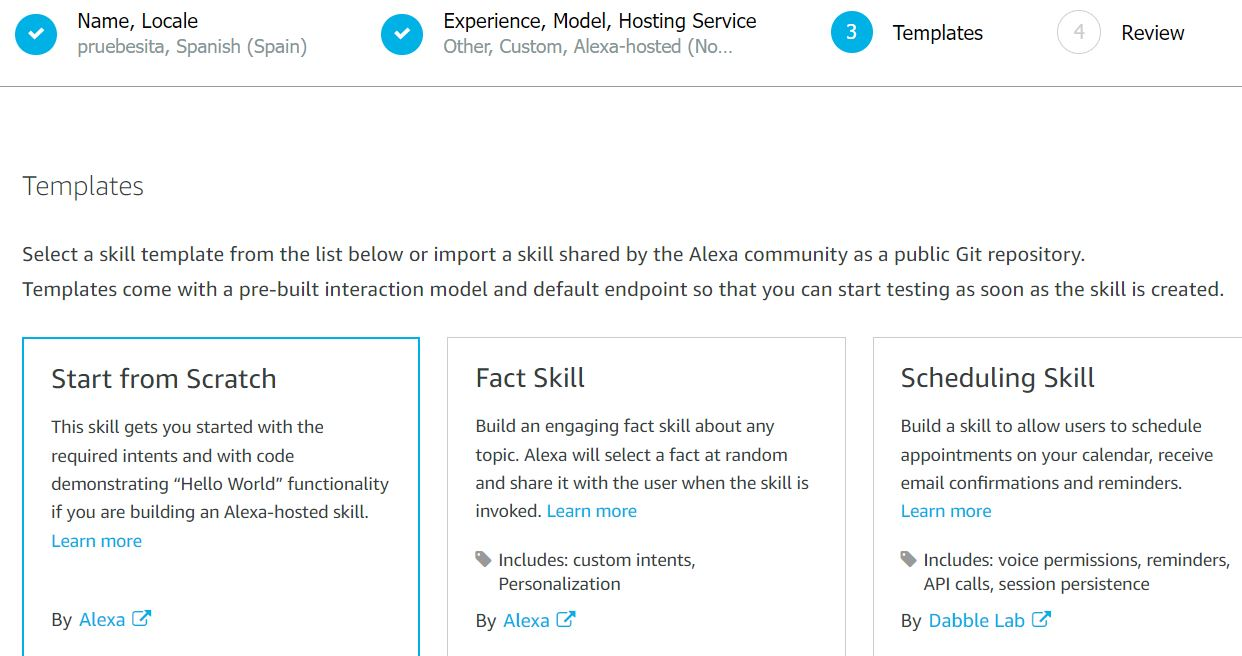
\includegraphics[width=1\textwidth]{imgs/alexa-dev-console-2.jpg}
	\caption{Menú de creación de una skill de Alexa}
	\label{fig:alexa-dev-console-2}
\end{figure}

Una vez creada y finalizada la configuración básica, se abrirá automáticamente el menú de \textit{Build}, desde el que se pueden ajustar varios aspectos de la skill.

Lo primero es declarar el nombre de invocación, que es con el que se llamará a la función de lanzamiento en el momento en el que se abre la skill, y se puede ajustar desde el menú lateral de \textit{Invocations}. Alexa establece una serie de restricciones sobre este parámetro: no puede incluir artículos o preposiciones, debe componerse de mínimo dos palabras, si contiene números estos deben ser escritos de manera completa, no debe incluir mayúsculas ni palabras reservadas como \enquote{Alexa, skill, app,} etc. 

El nombre de invocación elegido es \enquote{probando oca}, por tanto cuando se quiera iniciar la skill, habrá que decir: \enquote{Alexa, abre probando oca}.

Otro elemento desplegable revelante del menú lateral es el modelo de interacción (\textit{Interaction Model}), donde se definen los \textit{intents}. Inicialmente hay cinco predeterminados, de los cuales cuatro son de carácter obligatorio y por tanto no pueden borrarse:

\begin{itemize}
	\item \textbf{AMAZON.CancelIntent}: cancela la acción actual y termina la interacción con la skill.
	\item \textbf{AMAZON.HelpIntent}: proporciona información sobre cómo usar la habilidad.
	\item \textbf{AMAZON.StopIntent}: detiene la acción en curso y finaliza la interacción con la skill.
	\item \textbf{AMAZON.NavigateHomeIntent}: regresa al inicio de o a la pantalla principal.
	\item \textbf{HelloWorldIntent}: ejecuta la acción personalizada predefinida, que consiste en saludar a la persona usuaria. Es la única que puede eliminarse.
\end{itemize}

También se puede acceder y modificar el archivo JSON del modelo de interacción directamente, aunque es aconsejable utilizar en lugar de ello la interfaz de configuración, ya que cada vez que se monta la skill este fichero se actualiza automáticamente.

Otro elemento interesante son los Assets, que permiten la creación de tipos personalizados de slots, la consulta del historial de compilación de la skill y la configuración del \textit{endpoint}. 

Al tratarse de una skill alojada por Alexa, el endpoint se trata de la función Lambda de AWS encargada de la ejecución del código de la skill. Además, por defecto se dispone de tres de ellos, localizados en distintas regiones del mundo: Virginia del Norte, Irlanda y Oregon.

\begin{figure}[H]
	\centering
	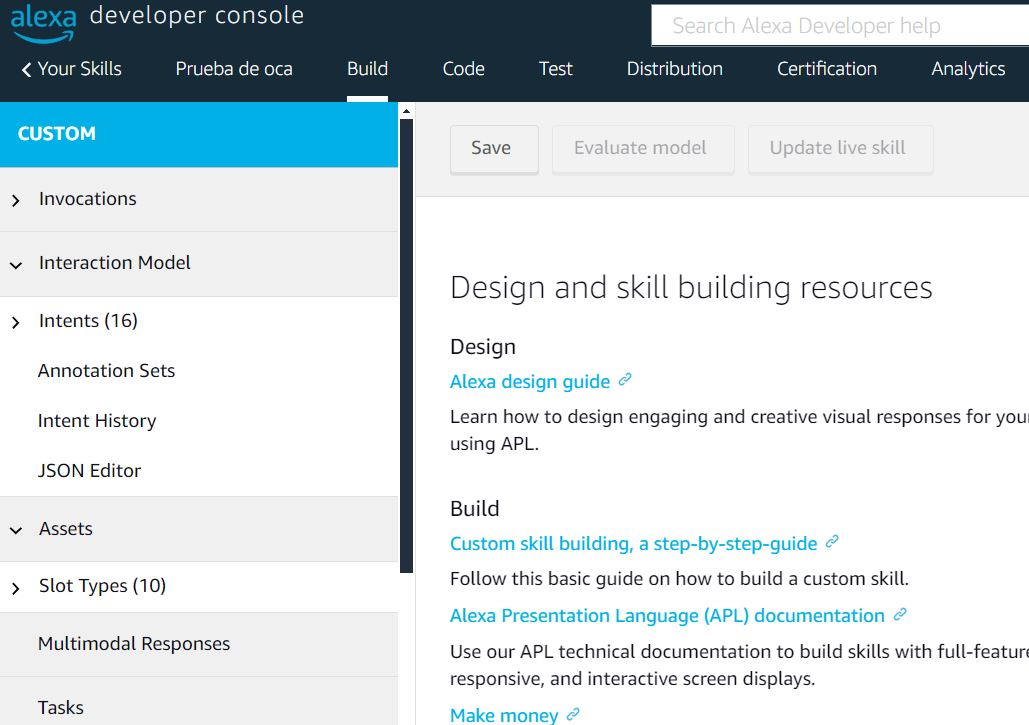
\includegraphics[width=1\textwidth]{imgs/alexa-dev-console-1.jpg}
	\caption{Menú principal de montaje de la skill de Alexa}
	\label{fig:alexa-dev-console-1}
\end{figure}

Si se navega al menú de código desde la barra de herramientas, se puede encontrar la siguiente estructura de archivos:

\begin{figure}[H]
	\centering
	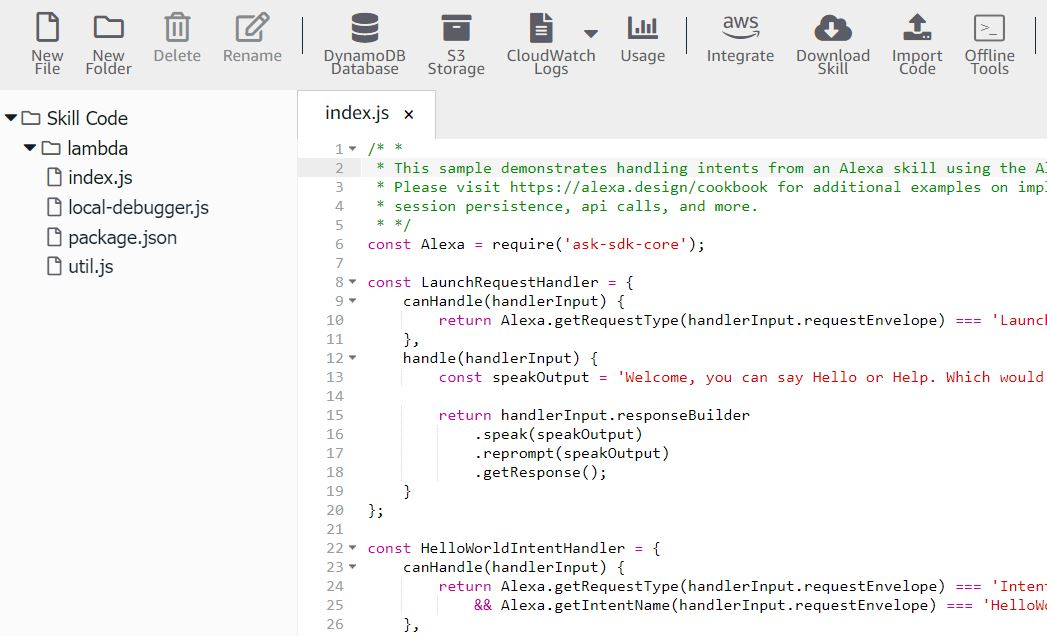
\includegraphics[width=1\textwidth]{imgs/alexa-dev-console-3.jpg}
	\caption{Menú del código de la skill de Alexa}
	\label{fig:alexa-dev-console-3}
\end{figure}

El fichero \textit{index.js} es el más importante, ya que actúa como entrypoint o punto de entrada de la skill, donde se exporta la función de Lambda. Es el que gestiona todos los handlers (manejadores de solicitudes), que determinan el flujo de conversación de Alexa gracias a la capacidad de establecer respuestas concretas a cada intent. Los handlers predefinidos son:
\begin{itemize}
	\item \textbf{LaunchRequestHandler}:  se activa cuando se abre la skill sin especificar un comando, respondiendo con un mensaje de bienvenida.
	\item \textbf{HelloWorldIntentHandler}: responde cuando el usuario invoca a \textit{HelloWorldIntent}, que se limita a saludar.
	\item \textbf{HelpIntentHandler}: maneja el \textit{AMAZON.HelpIntent}, puede invocarse cuando se necesita ayuda.
	\item \textbf{CancelAndStopIntentHandler}: gestiona \textit{AMAZON.CancelIntent} y \textit{AMAZON.StopIntent}, que sirve para detener la skill.
	\item \textbf{FallbackIntentHandler}: se activa se dice algo que no coincide con ninguno de los intents definidos.
	\item \textbf{SessionEndedRequestHandler}: se invoca cuando una sesión termina, ya sea por un comando de usuario o error.
	\item \textbf{IntentReflectorHandler}: útil para la depuración de la skill, ya que responde con el nombre del intent con el que fue llamado. 
	\item \textbf{ErrorHandler}: sirve para la captura de errores de cualquier tipo.
\end{itemize}

Otro archivo esencial en cualquier proyecto realizado con Node.js es \textit{package.json}, donde se definen las dependencias y bibliotecas requeridas, además de permitir la configuración de scripts, pruebas e información acerca de la versión, nombre del proyecto, etc.

Por otro lado, los dos ficheros restantes (\textit{local-debugger.js} y \textit{util.js}) no han sido necesarios para el desarrollo del proyecto, pero pueden servir como base para facilitar la depuración local de la skill y definir funciones de utilidad generales.

\subsection{Configuración de servicios de AWS}

La plataforma de servicios AWS ofrece una amplia gama de mecanismos de monitorización, almacenamiento, gestión de políticas, computación, etc. Se caracteriza, entre otras cosas, por la flexibilidad y escalabilidad que permite gracias a su modelo de \enquote{pagar solo lo que se usa}.

En la consola de desarrolladores de AWS aparecen todos los servicios usados recientemente, facilitando la navegación entre ellos.

\begin{figure}[H]
	\centering
	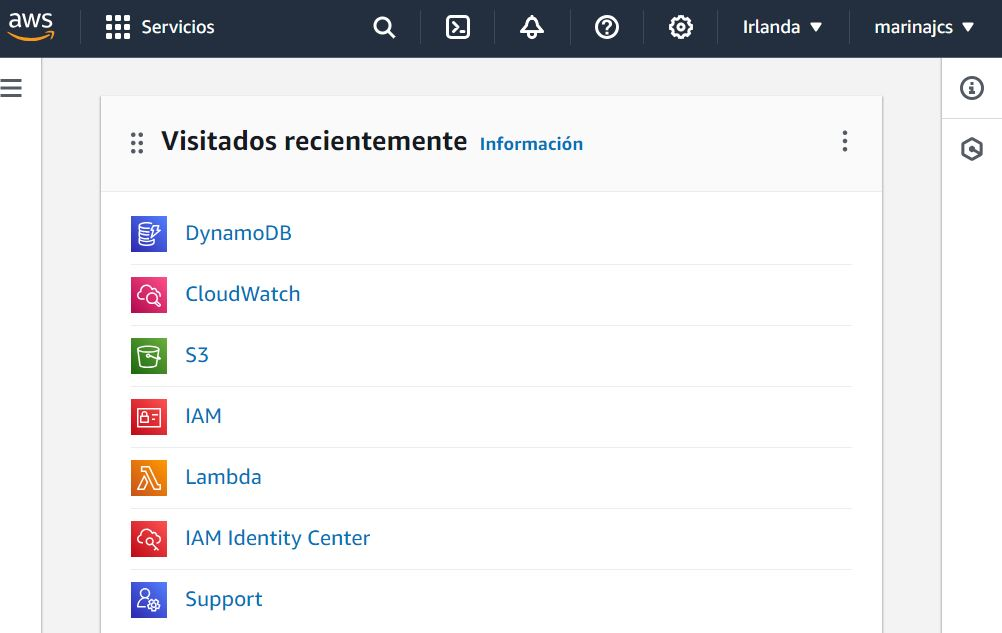
\includegraphics[width=0.7\textwidth]{imgs/aws-console-1.jpg}
	\caption{Menú de la consola de desarrolladores de AWS}
	\label{fig:aws-console-1}
\end{figure}


\subsubsection{Identity and Access Management (IAM)}

El primer servicio utilizado es IAM, con el objetivo de crear un rol capaz de otorgar permisos temporales de acceso a DynamoDB a skills de Alexa.

\begin{figure}[H]
	\centering
	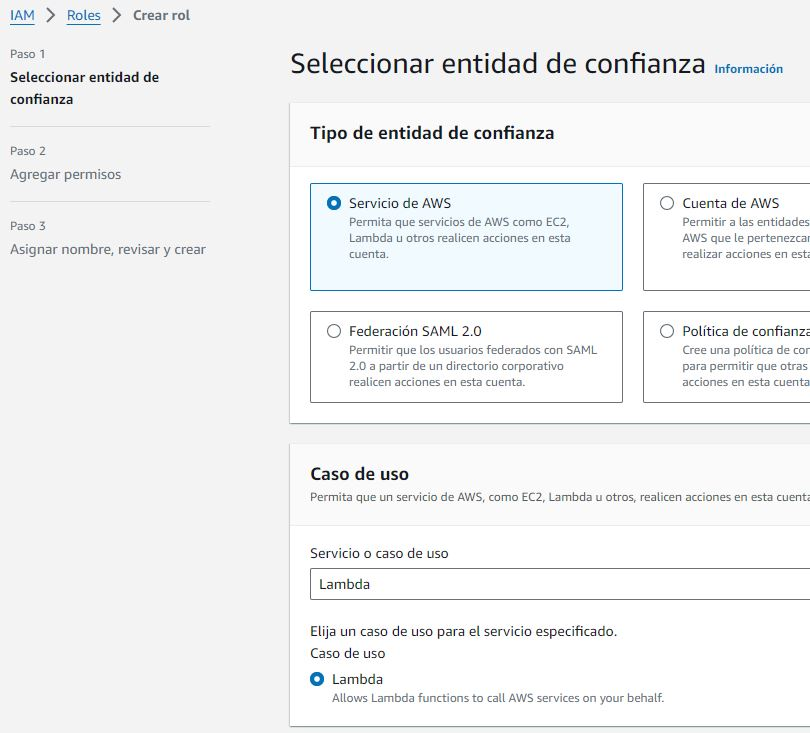
\includegraphics[width=1\textwidth]{imgs/aws-iam-2.jpg}
	\caption{Menú de creación de un rol IAM}
	\label{fig:aws-iam-2}
\end{figure}

En el menú de creación del rol, hay que rellenar los siguientes parámetros de configuración: el tipo de entidad de confianza (un servicio de AWS), el caso de uso (la función de Lambda), las políticas de permisos a agregar (\textit{AmazonDynamoDBFullAccess}) y el nombre del rol que se está creando.

\begin{figure}[H]
	\centering
	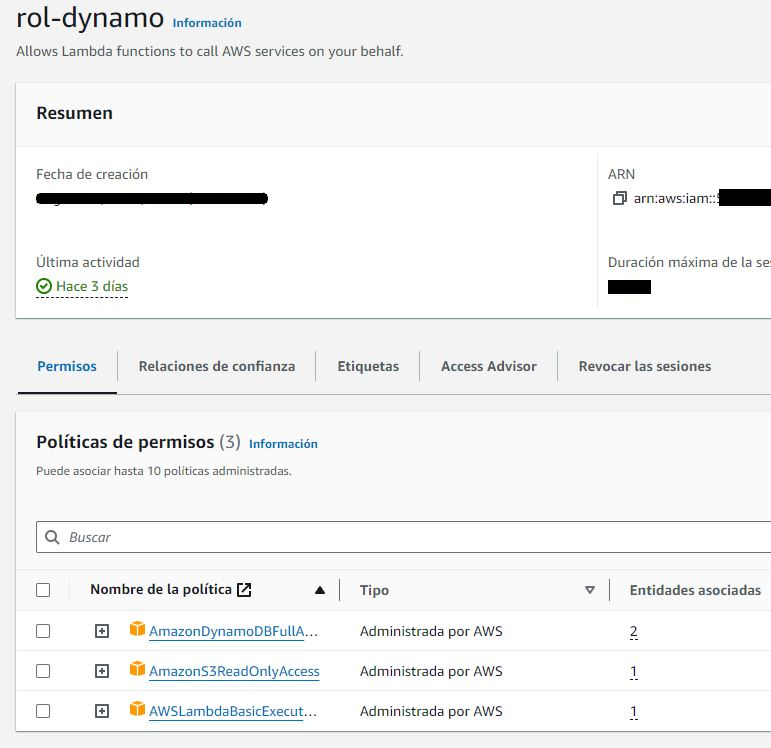
\includegraphics[width=1\textwidth]{imgs/aws-iam-1.png}
	\caption{Rol creado para la skill y sus permisos en AWS}
	\label{fig:aws-iam-1}
\end{figure}

Para que la skill pueda usar los recursos de AWS que será definidos en las secciones siguientes, se necesita modificar el fichero JSON que especifica las relaciones de confianza del rol. Para ello, se añade la siguiente entrada:

\begin{figure}[H]
	\centering
	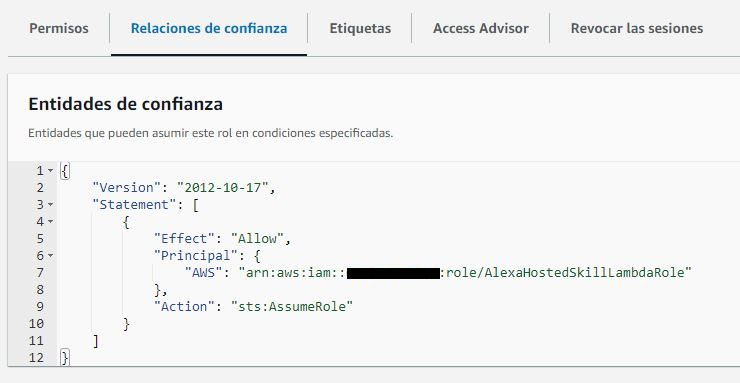
\includegraphics[width=1\textwidth]{imgs/aws-iam-3.png}
	\caption{Configuración de las relaciones de confianza del rol}
	\label{fig:aws-iam-3}
\end{figure}

El texto censurado es el ARN (Amazon Resource Name) o identificador del rol de ejecución IAM que la función Lambda asume al ejecutarse la skill de Alexa. Este se puede obtener desde la consola de desarrolladores de Alexa, en el menú del código, con la opción \textit{Integrate}, especialmente diseñada para poder vincular la skill a servicios personales de AWS.

\begin{figure}[H]
	\centering
	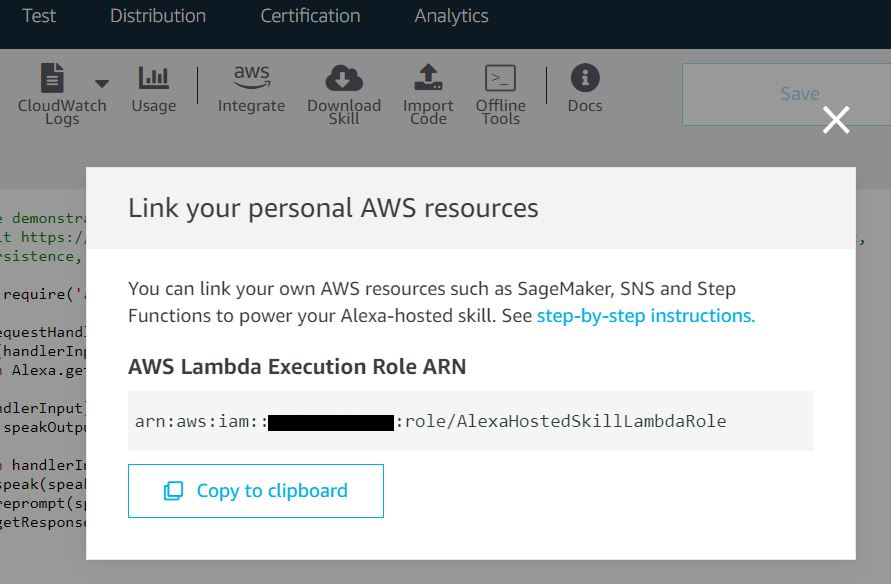
\includegraphics[width=0.75\textwidth]{imgs/aws-iam-4.png}
	\caption{El AWS Lambda Execution Role ARN de la skill}
	\label{fig:aws-iam-4}
\end{figure}

\subsubsection{Amazon Simple Storage Service (S3)}

Como su nombre indica, es un servicio ofrecido en AWS que permite almacenar objetos de diversos tipos (textos, binarios, documentos, audios, comprimidos, etc). Sin embargo, dados los requisitos de este juego, solo será necesario guardar lo siguiente: las imágenes asociadas a cada casilla, la de la pantalla de bienvenida y los vídeos con las animaciones de los lanzamientos de dado.

En Amazon S3, se ha adoptado el término de \textit{bucket} como un contenedor para almacenar objetos. Cada bucket tiene un nombre único y puede simular una estructura de directorios, además pueden ser de acceso público o privado, al igual que sus elementos, que pueden configurarse a través de políticas de acceso.

Para este proyecto, se ha creado un bucket de nombre \textit{bucket-oca} para guardar todos los archivos multimedia que necesita la skill.

\begin{figure}[H]
	\centering
	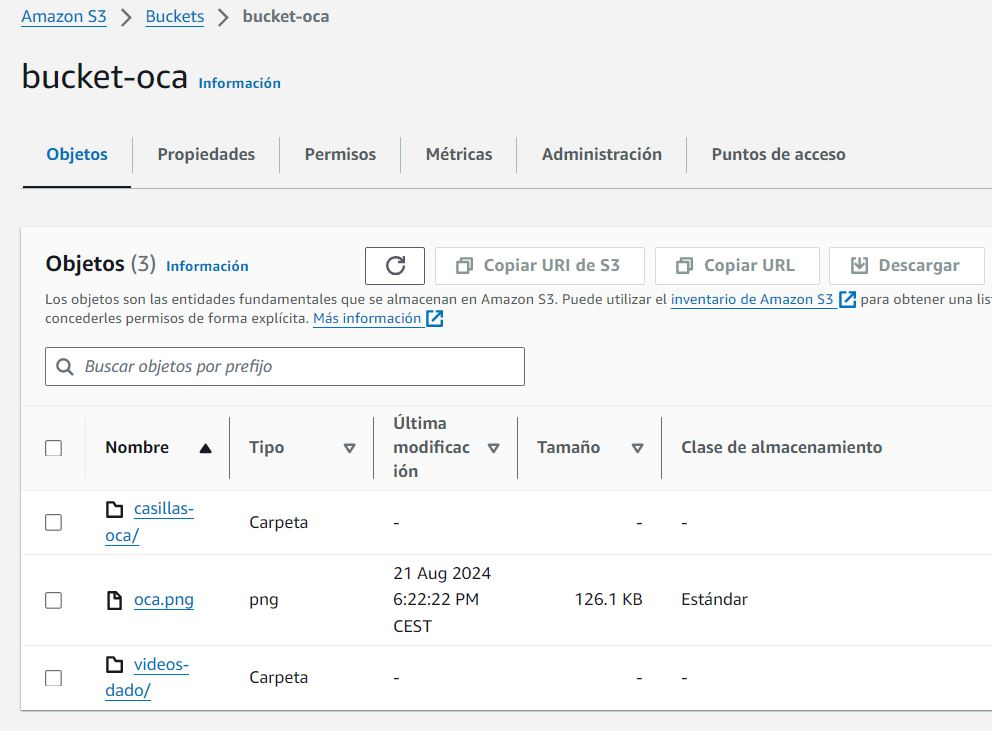
\includegraphics[width=1\textwidth]{imgs/aws-s3-1.jpg}
	\caption{Bucket de Amazon S3 para la skill de la oca}
	\label{fig:aws-s3-1}
\end{figure}

\subsubsection{DynamoDB}

Como se ha mencionado en la sección \textit{6.1.2.}, los datos de una skill no persisten de una sesión a otra, por lo que es necesario un mecanismo para guardarlos. Aquí entra el papel de las bases de datos, en particular DynamoDB, también intergado en AWS.

Esta base de datos es de tipo NoSQL y es una alternativa interesante no solo por su total compatibilidad con las herramientas actuales del proyecto debido a que es otro servicio Amazon, sino también por su alta capacidad de adaptación a cualquier volumen de datos. 

Es conocido por optimizar sus tiempos de respuesta y llevar a cabo un escalado automático en función del tráfico, gracias a su esquema NoSQL, cuyos elementos de las tablas se identifican mediante claves primarias únicas. Estas últimas pueden ser de partición o compuestas (unión de una clave de partición con una de ordenamiento). Para este proyecto, se han creado dos tablas: 
\begin{itemize}
	\item \textbf{JuegoOca}: su clave primaria es \textit{idJuego}, que siempre valdrá 0 debido a que se pretende guardar los datos de una sola partida entre sesiones. Tiene los elementos generales de un juego de la oca, que son el estado, el turno y ronda actual, el número de jugadores, el tipo de participantes...
	\item \textbf{Jugador}: identificada por la clave primaria \textit{idJugador}, que a la vez determina el orden de turno, y será un valor entero único entre 0 y el el numero de total de participantes menos uno. Los atributos de cada elemento son: el nombre, el color, los puntos, la posición y penalizaciones actuales, etc.
\end{itemize} 

\begin{figure}[H]
	\centering
	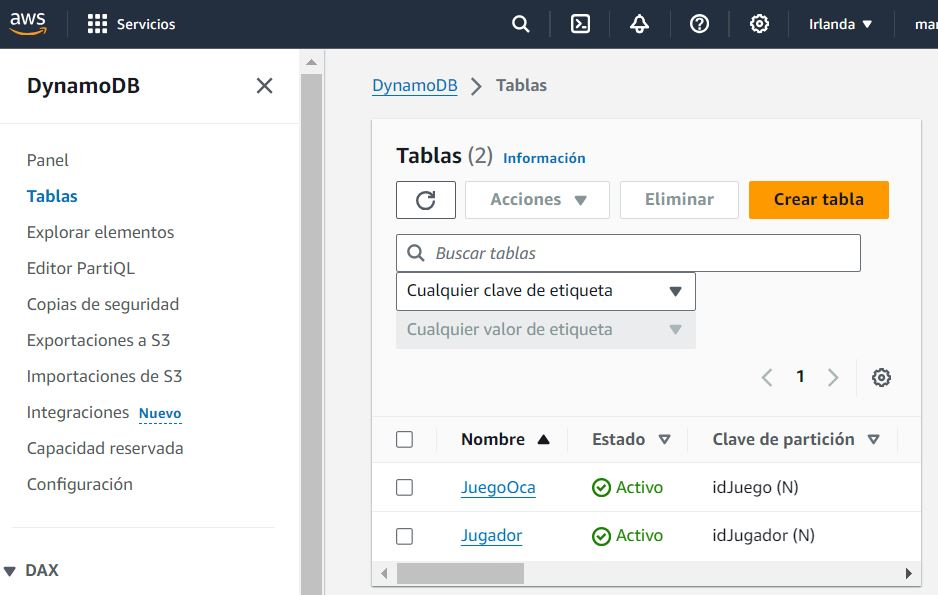
\includegraphics[width=0.8\textwidth]{imgs/aws-db-1.jpg}
	\caption{Tablas \textit{JuegoOca} y \textit{Jugador} creadas en DynamoDB}
	\label{fig:aws-db-1}
\end{figure}

Desde la consola de AWS, dentro del servicio de DynamoDB, se pueden explorar los elementos guardados en las tablas, así como consultar las unidades de lectura/escritura consumidas hasta el momento.

\begin{figure}[H]
	\centering
	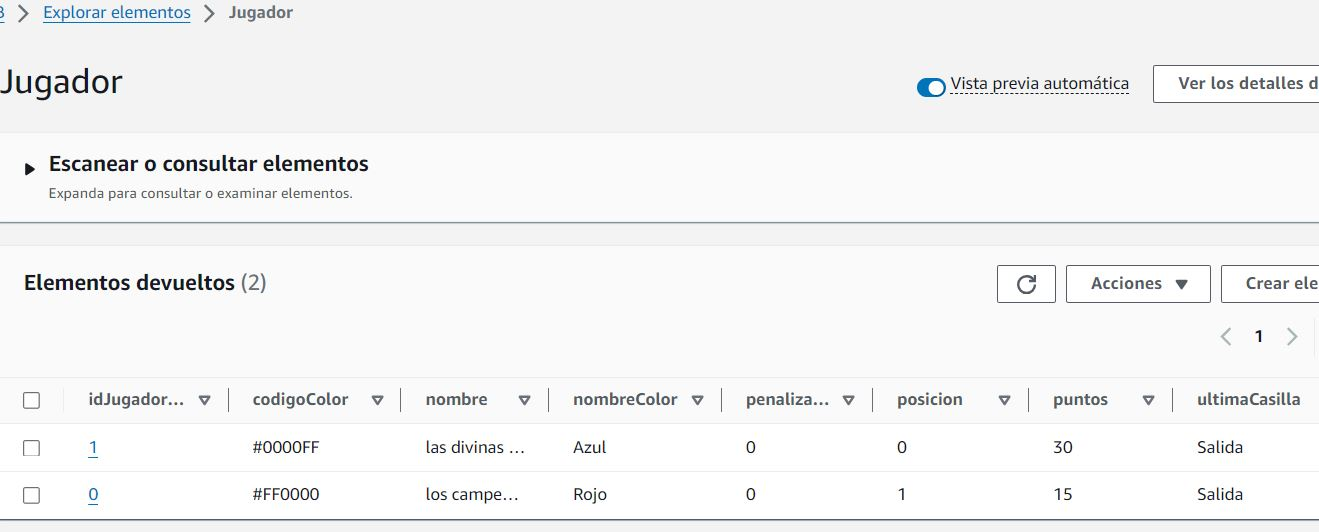
\includegraphics[width=1\textwidth]{imgs/aws-db-2.jpg}
	\caption{Información de la tabla \textit{Jugador} de DynamoDB}
	\label{fig:aws-db-2}
\end{figure}

\subsection{Implementación y estructura del código}

La estructura de archivos del código de la función de Lambda que ejecuta la skill del juego es la siguiente:

\begin{figure}[H]
	\centering
	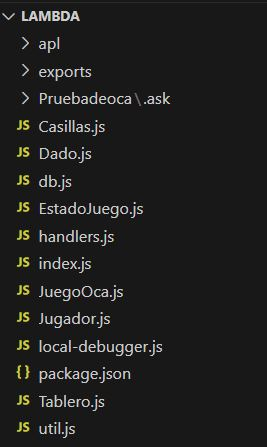
\includegraphics[width=0.3\textwidth]{imgs/estructura-codigo.jpg}
	\caption{Estructura del código de la función Lambda}
	\label{fig:estructura-codigo}
\end{figure}

A continuación se explicarán los contenidos de los ficheros, salvo: \textit{local-debugger.js}, \textit{package.json} y \textit{util.js}, que ya fueron descritos en la sección \textit{7.1.}

\subsubsection{Lógica del juego de la oca}

Consiste en la implementación de las clases definidas en el modelo conceptual de la sección \textit{5.3}, que cubren las funcionalidades del juego de la oca.

\paragraph{Fichero \enquote{Jugador.js}}

Define la clase encargada de representar a cada participante, ya sea un equipo o jugador/a individual, que va a competir en el juego de la oca.

\begin{figure}[H]
	\centering
	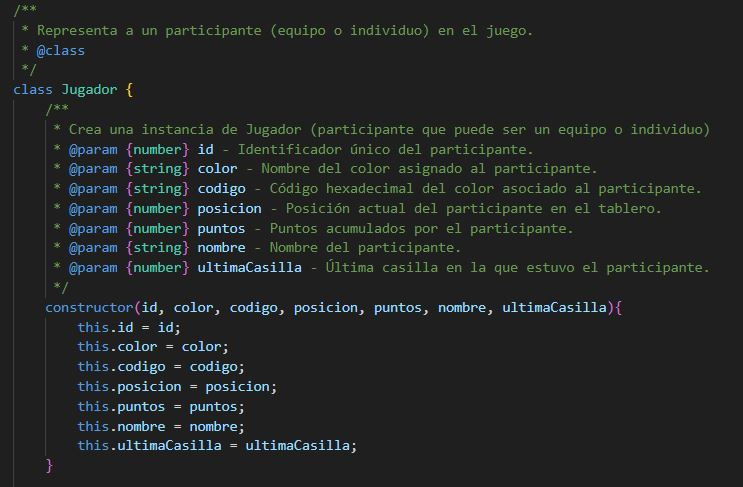
\includegraphics[width=0.8\textwidth]{imgs/codigo-jugador.jpg}
	\caption{Clase jugador junto con su constructor}
	\label{fig:codigo-jugador}
\end{figure}

También incluye \textit{setters} y \textit{getters} para poder modificar y consultar cada atributo de clase.

\paragraph{Fichero \enquote{Dado.js}}

Está constituido por dos funciones auxiliares: la primera, que realiza un lanzamiento de dado, devolviendo un número aleatorio entre 1 y 6, y la segunda, para obtener la dirección URL del vídeo asociado a cada resultado posible de una tirada. Esto será especialmente útil cuando se vaya a implementar el APL más adelante.

\begin{figure}[H]
	\centering
	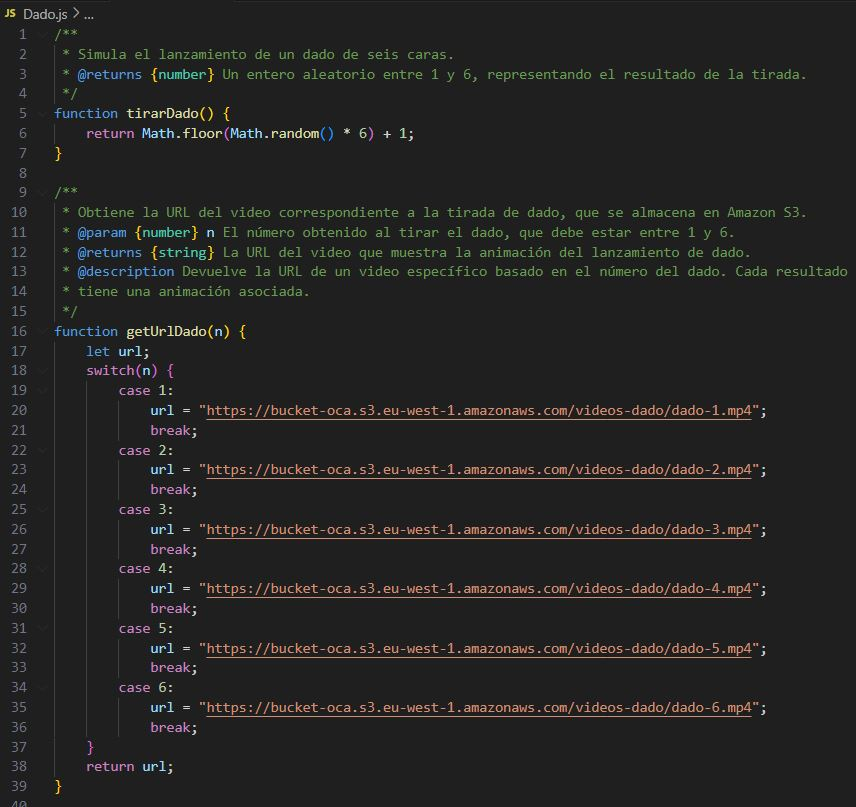
\includegraphics{imgs/codigo-dado.jpg}
	\caption{Funciones que componen el módulo del dado}
	\label{fig:codigo-dado}
\end{figure}

\paragraph{Fichero \enquote{Casillas.js}}

En las primeras líneas se realizan las importaciones necesarias de los datos de las preguntas que se usarán para los minijuegos, así como las frases de carácter descriptivo que se invocarán cuando se caiga en cualquier casilla.

\begin{figure}[H]
	\centering
	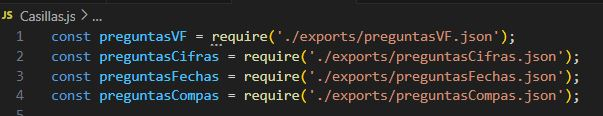
\includegraphics[width=0.8\textwidth]{imgs/codigo-casillas-1.jpg}
	\caption{Importaciones de las baterías de preguntas de los minijuegos}
	\label{fig:codigo-casillas-1}
\end{figure}

\newpage
Luego, se define la clase que representa una casilla general (o de carácter normal); es decir, aquella que no desencadena ningún evento especial como desplazarse a otra casilla, tirar el dado de nuevo, iniciar un minijuego, etc.

\begin{figure}[H]
	\centering
	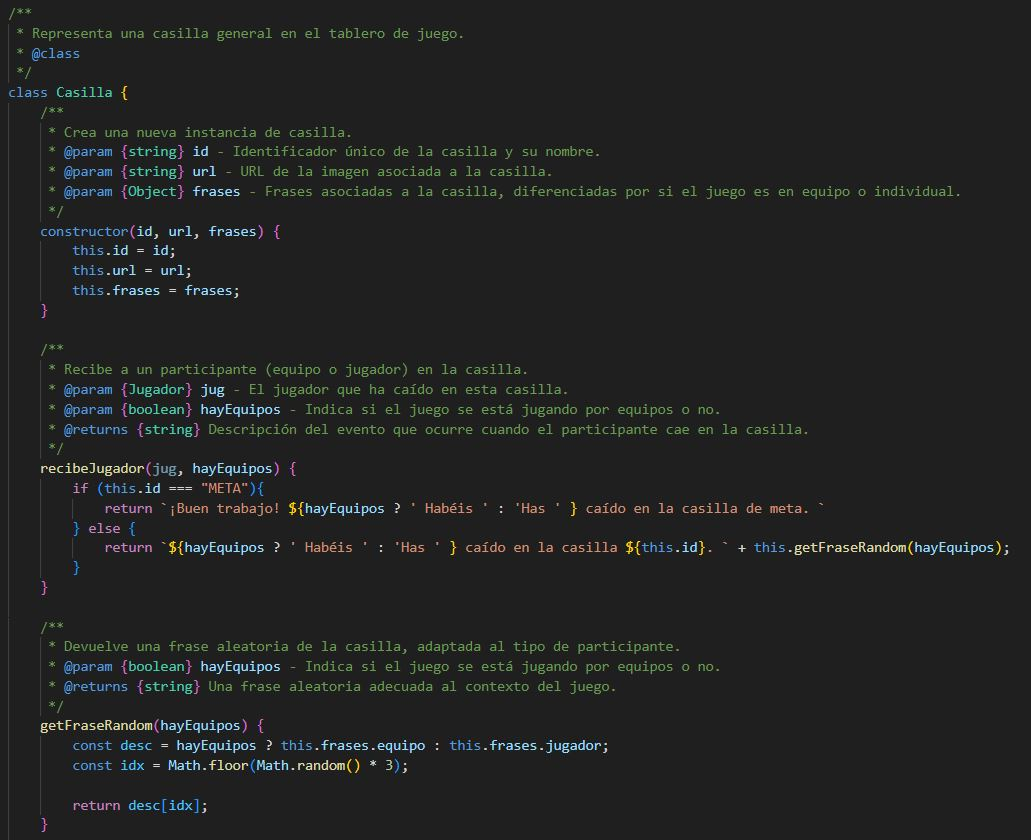
\includegraphics[width=1\textwidth]{imgs/codigo-casillas-2.jpg}
	\caption{Declaración de la clase de una casilla normal}
	\label{fig:codigo-casillas-2}
\end{figure}

Se puede ver cómo hay dos métodos: \textit{getFraseRandom()}, encargado de devolver una descripción aleatoria de la casilla normal, habiendo tres posibles opciones para cada una, y \textit{recibeJugador()}, que informa al participante sobre dónde ha caído, incluyendo la descripción de la misma. 
Este último método será sobrescrito en las distintas clases que heredan de \textit{Casilla}, para adaptar los informes en función del tipo de la instancia. Por ejemplo, si es una casilla de oca, dirá \enquote{de oca en oca y tiro porque me toca}, si es una de minijuego, anunciará qué tipo de pregunta hará y cómo jugar, etc.

\subparagraph{Casillas especiales tradicionales: oca, puente y penalización}

Siguiendo el esquema del juego de mesa tradicional, las casillas de oca permiten moverse a la siguiente del mismo y tirar el dado de nuevo; las casillas de puente, transportan a la otra casilla del mismo tipo independientemente de si dicho movimiento supone un avance o retroceso en el tablero; y las casillas de penalización, como la del pozo y el laberinto, hacen perder turnos a cualquiera que caiga en ellas.

Las casillas de oca y de puente mantienen una estructura similar a su superclase, con los mismos atributos y la única diferencia en el método sobrescrito de \textit{recibeJugador()}; sin embargo, la clase \textit{CasillaPenalizacion} incluye un nuevo atributo (\textit{penaliza}) que representa el número de turnos que deben pasar antes de poder avanzar de nuevo.

\begin{figure}[H]
	\centering
	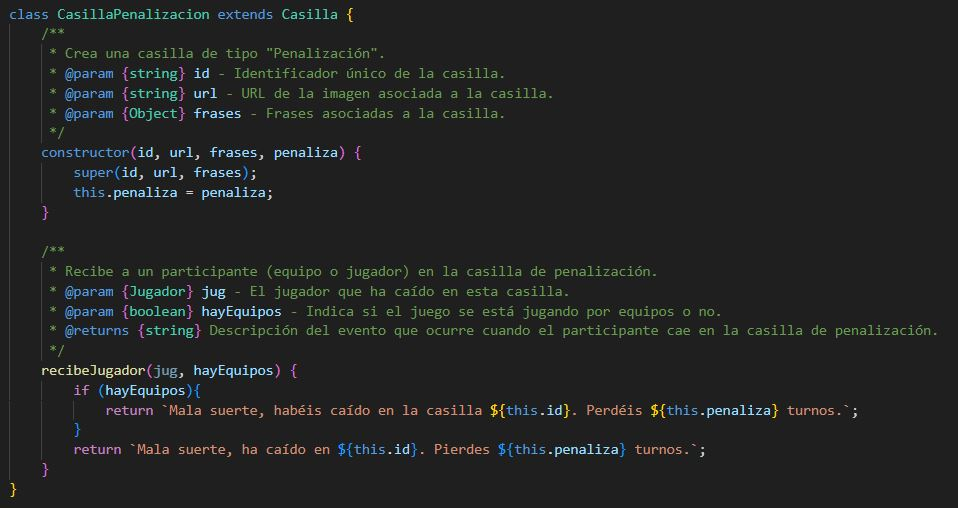
\includegraphics{imgs/codigo-casillas-3.jpg}
	\caption{Declaración de la clase de casillas de penalización}
	\label{fig:codigo-casillas-3}
\end{figure}

\subparagraph{Casillas de minijuegos personalizadas}

Se caracterizan porque además de los métodos heredados de las casillas normales, cuentan con un método llamado \textit{getPreguntaRandom()}, que devuelve un elemento aleatorio de la batería de preguntas del tipo correspondiente, con la excepción del minijuego de \enquote{recuerda la última casilla}, que no necesita el método porque la pregunta siempre es la misma.

Por tanto, la clase que define la casilla del minijuego de verdadero o falso tendría la siguiente apariencia:

\begin{figure}[H]
	\centering
	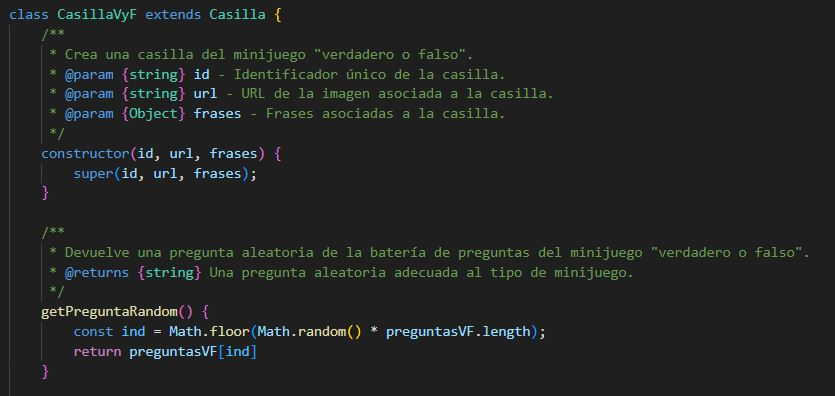
\includegraphics{imgs/codigo-casillas-4.jpg}
	\caption{Clase para casilla del minijuego verdadero o falso}
	\label{fig:codigo-casillas-4}
\end{figure}

En el minijuego de \enquote{conoce a tus compañeros} también se necesita guardar el nombre del equipo/participante sobre el que va la pregunta, así que sehace una ligera modificación, pasándole como argumento un arreglo con todos los compañeros del jugador o jugadora actual.

\begin{figure}[H]
	\centering
	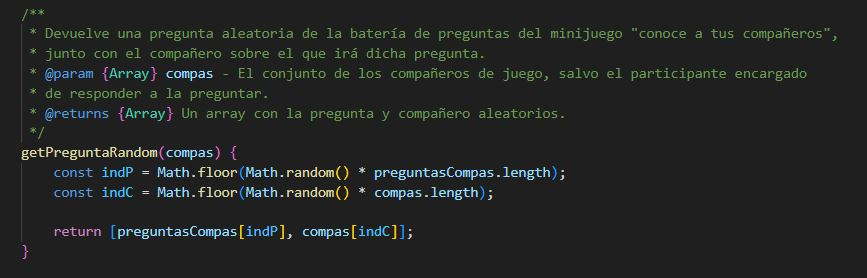
\includegraphics{imgs/codigo-casillas-5.jpg}
	\caption{Método para obtener una pregunta aleatoria sobre un compañero}
	\label{fig:codigo-casillas-5}
\end{figure}

Las clase para la casilla del minijuego \enquote{adivina la cifra} es parecida a la de la figura 44. Por otro lado, como en el minijuego de \enquote{recuerda la fecha} se manejan tres tipos distintos de preguntas y respuestas (día de la semana, mes o estación del año), y la solución correcta se calcula a partir de la fecha actual, o lo que es lo mismo, no es un valor estático, entonces requiere añadir una serie de métodos adicionales:

\begin{figure}[H]
	\centering
	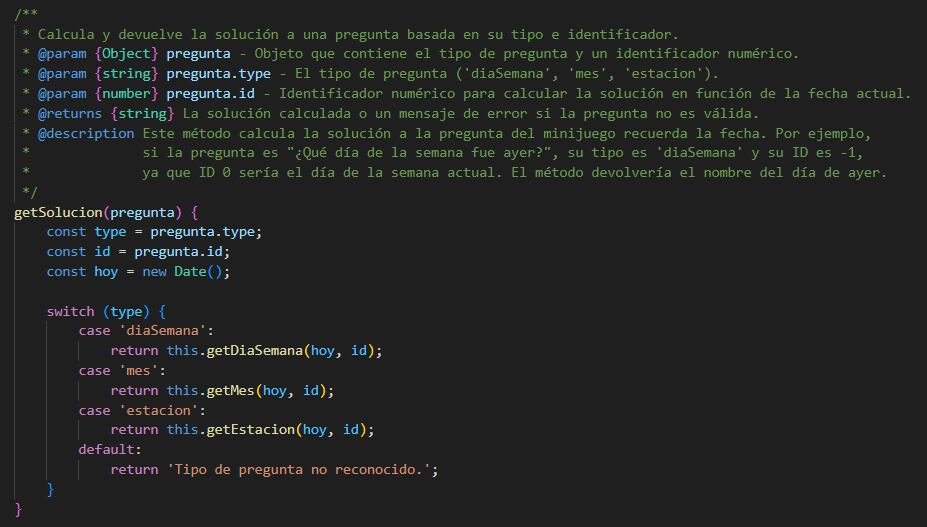
\includegraphics{imgs/codigo-casillas-6.jpg}
	\caption{Método para obtener la solución de una pregunta de fecha}
	\label{fig:codigo-casillas-6}
\end{figure}

En la figura anterior, aparecen invocaciones a tres métodos auxiliares que permiten el cálculo correcto de la respuesta pasándole como argumentos el valor de la fecha actual y un id o número de desplazamiento partiendo del actual. Si el id es igual a 0, entonces la solución es el día/mes/estación actual; si el id es 1, la respuesta es el día/mes/estación siguiente al actual; si el id es -1, el anterior al actual... Y así sucesivamente. 

\begin{figure}[H]
	\centering
	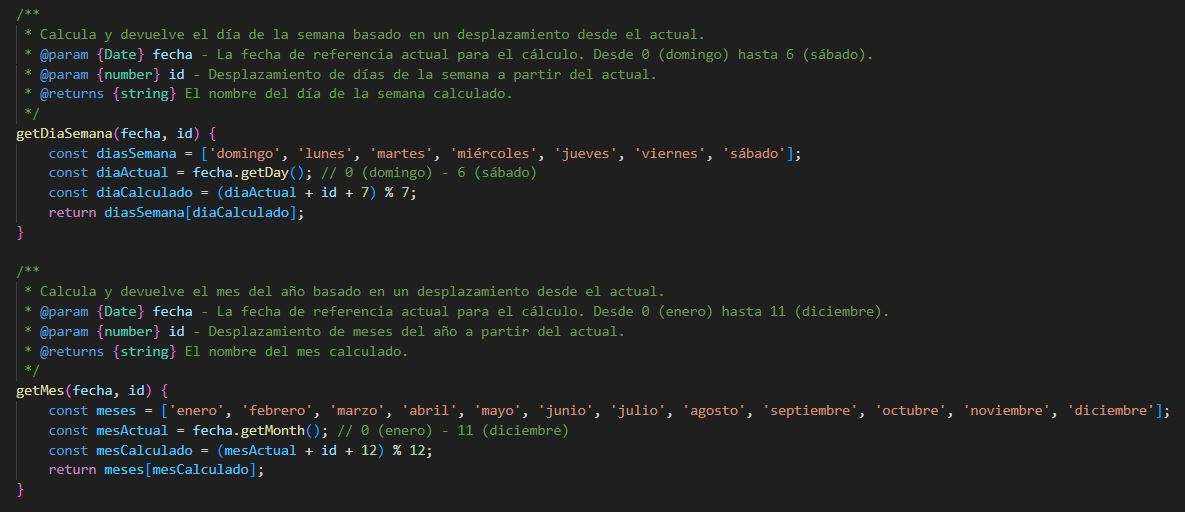
\includegraphics[width=1\textwidth]{imgs/codigo-casillas-7.jpg}
	\caption{Cálculo de días de la semana o meses a partir de la fecha actual}
	\label{fig:codigo-casillas-7}
\end{figure}

\begin{figure}[H]
	\centering
	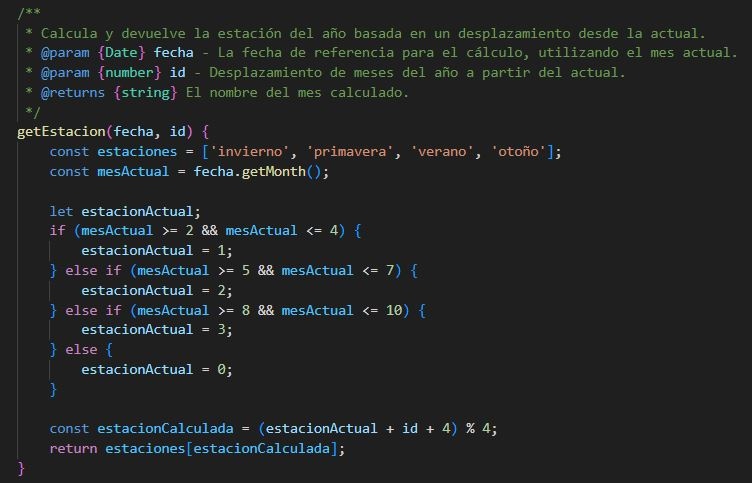
\includegraphics[width=0.82\textwidth]{imgs/codigo-casillas-8.jpg}
	\caption{Cálculo de la estación del año partiendo de la fecha actual}
	\label{fig:codigo-casillas-8}
\end{figure}

\paragraph{Fichero \enquote{Tablero.js}}

Es la estructura que almacena todas las casillas del juego en un arreglo con el mismo nombre, y hace operaciones básicas de gestión como añadir nuevas casillas u obtener una concreta a partir de un índice.

\begin{figure}[H]
	\centering
	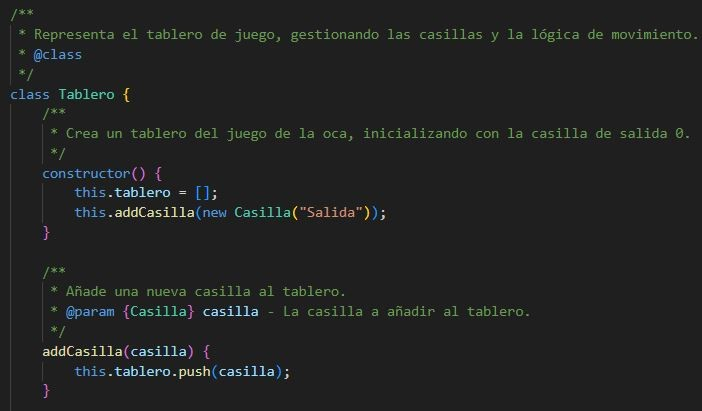
\includegraphics[width=0.82\textwidth]{imgs/codigo-tablero-1.jpg}
	\caption{Declaración de la clase Tablero}
	\label{fig:codigo-tablero-1}
\end{figure}

\newpage
Además, es la encargada de calcular una nueva posición a partir del índice de la casilla actual y el número de desplazamiento, asegurándose de que si es mayor que el número de casillas restantes hasta la meta, pueda retroceder y no salirse del límite.

Otra de sus funcionalidades es la de buscar la siguiente casilla de tipo oca, dada la posición de la actual, útil para manejar el evento cuando se cae en una. También cuenta con un método para obtener la otra casilla de puente.

\begin{figure}[H]
	\centering
	\includegraphics[width=0.9\textwidth]{imgs/codigo-tablero-2.jpg}
	\caption{Métodos para calcular una posición y buscar un tipo de casilla}
	\label{fig:codigo-tablero-2}
\end{figure}

\newpage
\paragraph{Fichero \enquote{EstadoJuego.js}}

Aquí va el contenido del párrafo.

\begin{figure}[H]
	\centering
	\includegraphics{imgs/codigo-estado-1.jpg}
	\caption{Simula la estructura de datos \textit{enum} de los estados del juego}
	\label{fig:codigo-estado-1}
\end{figure}

\begin{figure}[H]
	\centering
	\includegraphics{imgs/codigo-estado-2.jpg}
	\caption{Función que devuelve un mensaje de ayuda según el estado del juego}
	\label{fig:codigo-estado-2}
\end{figure}

\paragraph{Fichero \enquote{JuegoOca.js}}

Es la clase más extensa de todas, haciendo uso del resto de clases definidas anteriormente, lo que puede observarse en los módulos que han tenido que importarse.

\begin{figure}[H]
	\centering
	\includegraphics{imgs/codigo-oca-1.jpg}
	\caption{Importaciones y declaración de la clase del juego de la oca}
	\label{fig:codigo-oca-1}
\end{figure}

Esta clase dispone de varios de métodos para implementar la lógica del juego:

\begin{itemize}
	\item \textbf{crearJugadores()}: crea un número específico de jugadores (hasta 5), asignándoles colores y códigos únicos (salvo los nombres, que serán añadidos más tarde), inicializándolos con los valores de partida predeterminados, y actualizando el estado de juego.
	\begin{figure}[H]
		\centering
		\includegraphics{imgs/codigo-oca-2.jpg}
		\caption{Método de inicialización de participantes del juego}
		\label{fig:codigo-oca-2}
	\end{figure}
	
	\item \textbf{crearTablero()}: genera un tablero completo con 63 casillas, con diferentes tipos como CasillaOca, CasillaPenalizacion, CasillaVyF, entre otras, para un juego completo de la oca.
	\begin{figure}[H]
		\centering
		\includegraphics[width=1\textwidth]{imgs/codigo-oca-3.jpg}
		\caption{Método de inicialización del tablero de la oca}
		\label{fig:codigo-oca-3}
	\end{figure}
	
	\item \textbf{pasarTurno()}: avanza el turno, recalcula el número de ronda, actualiza el estado del juego y devuelve un mensaje anunciando el turno del siguiente participante. comprobando antes si tiene penalizaciones de turno o no.
	\begin{figure}[H]
		\centering
		\includegraphics{imgs/codigo-oca-5.jpg}
		\caption{Método para pasar al siguiente turno}
		\label{fig:codigo-oca-5}
	\end{figure} 
	
	\item \textbf{anunciarGanadores()}: si el juego ha finalizado, devuelve u mensaje anunciando las dos modalidades de ganadores: quien haya llegado antes a la meta y quien haya obtenido más puntos gracias a los minijuegos.
	\begin{figure}[H]
		\centering
		\includegraphics[width=1\textwidth]{imgs/codigo-oca-6.jpg}
		\caption{Método para anunciar los ganadores al final del juego}
		\label{fig:codigo-oca-6}
	\end{figure} 
	 
	\item \textbf{avanzarJugador()}: mueve al participante actual una cantidad determinada de casillas, actualizando su posición y manejando eventos específicos basados en el tipo de casilla en la que cae. También genera un informe sobre el movimiento realizado y actualiza el estado de la partida. \newline
	
	\begin{figure}[H]
		\centering
		\includegraphics{imgs/codigo-oca-4.jpg}
		\caption{Primeras líneas del método para avanzar las fichas}
		\label{fig:codigo-oca-4}
	\end{figure}
	
	\item Métodos \textit{getters} y \textit{setters} de todos los atributos de la clase.
	\item Métodos adicionales para calcular y hallar: un participante de índice concreto, el equipo o jugador/a del turno actual, sus compañeros de juego, los que se encuentran en una casilla determinada, las penalizaciones de alguno en particular, etc.
\end{itemize}

\subsubsection{Fichero \enquote{handlers.js}}

Con diferencia el fichero más extenso, con unas 900 líneas de código

\begin{figure}[H]
	\centering
	\includegraphics[width=1\textwidth]{imgs/codigo-handlers-1.jpg}
	\caption{Importaciones de bibliotecas y módulos para los handlers}
	\label{fig:codigo-handlers-1}
\end{figure}

De la siguiente lista de handlers definidos, se van a explicar todos los que han sido personalizados de alguna forma, exceptuando aquellos mencionados en la sección \textit{7.1.} que no hayan sufrido ningún cambio.
\begin{figure}[H]
	\centering
	\includegraphics[width=0.4\textwidth]{imgs/codigo-handlers-2.jpg}
	\caption{Todos los handlers que se exportan al \textit{index.js}}
	\label{fig:codigo-handlers-2}
\end{figure}

Cabe mencionar que cada handler está vinculado a un intent con el mismo nombre, que es invocado mediante utterances. Por ejemplo: con la utterance \enquote{Nueva partida}, se activa la intención \textit{nuevaPartidaIntent}, que provocará la ejecución del manejador \textit{nuevaPartidaHandler}, devolviendo una respuesta procesada a la persona usuaria.

\paragraph{\textit{LaunchRequestHandler}}

Este handler se activa cuando el usuario abre la skill por primera vez, mediante el comando \enquote{Alexa, abre probando oca}. Su función principal es dar una bienvenida al usuario y proporcionar opciones iniciales sobre cómo comenzar una partida. Informa al usuario sobre la posibilidad de continuar una partida previamente guardada o iniciar una nueva, advirtiendo que al comenzar una nueva se sobrescribirá la partida anterior. 

Si el dispositivo donde se ejecuta dispone de pantalla, se muestra la pantalla de inicio/bienvenida. Finalmente, el handler prepara una respuesta para que el usuario se sienta guiado sobre los próximos pasos, manteniendo la sesión activa para una interacción más fluida.

\paragraph{\textit{configuracion1Handler}}

Se invoca cuando el usuario solicita un intent específico para configurar una partida de prueba, útil para el proceso de depuración de errores y testeo de la skill. Este handler omite el proceso normal de configuración del juego y establece un estado predeterminado con dos equipos ficticios con nombres y puntos predefinidos para facilitar las pruebas. 

A continuación, notifica al usuario que la partida ha comenzado y le recuerda los comandos necesarios para jugar. Además, muestra información visual sobre los jugadores utilizando directivas APL.

\paragraph{\textit{guardarPartidaHandler} y \textit{cargarPartidaHandler}}

El primero responde a la solicitud de guardar el progreso actual del juego. A través de un rol temporal en AWS, accede a DynamoDB y almacena los datos de la partida en curso. Una vez que la partida se guarda correctamente, confirma el éxito o fracaso de la operación.

El segundo realiza el proceso inverso, pues se activa cuando el usuario desea cargar una partida previamente guardada. Vuelve a asumir un rol IAM temporal para conectarse con DynamoDB y recuperar los datos de la partida guardada. Así, permite continuar jugando desde el última punto guardado. 

\paragraph{\textit{ayudasReglasHandler}}

Invocado cuando la persona usuaria solicita ayuda, mediante el comando \enquote{Explícame <tema>}.

Dependiendo del tema específico sobre el que se quiere recibir información (como reglas generales, casillas del tablero, minijuegos o comandos), el handler proporciona una explicación detallada. Como en el resto de handlers, mantiene la sesión activa para ofrecer asistencia continua y mejorar la experiencia del usuario.

\paragraph{\textit{nuevaPartidaHandler}}

Se encarga de crear una nueva partida cuando el usuario lo solicita. Primero, pregunta por el tipo de participación (individual o en equipos) y luego por el número de participantes desde los slots del intent. 

Una vez se han recibido los datos, y confirmado que son correctos, se actualiza el estado del juego y se proporciona una explicación sobre cómo proceder al registro los nombres, indicando el formato correcto y sugiriendo ejemplos. 

A partir de este punto, se tiene en cuenta el tipo de participación para ajustar todas las respuestas con menciones a los equipos o jugadores individuales. 

\paragraph{\textit{addJugadorHandler}}

Es el paso obligatorio que sigue al anterior handler, este gestiona el registro de nombres de los jugadores en el juego. Se activa cuando cada participante proporciona su nombre a través del comando \enquote{Mi/Nuestro nombre es <nombre>}. 

Primero, verifica si el estado del juego está en la fase de registro de nombres y después, guarda el nombre. Si aún faltan participantes por registrar, solicita el siguiente nombre, y una vez que haya recibido todos, hace un resumen de los jugadores o equipos y guarda los datos de partida configurados en DynamoDB. También muestra en pantalla mediante APL los nombres y colores de los participantes recién registrados.

Por último, informa al usuario que la partida está lista para comenzar y guía sobre los próximos pasos: el lanzamiento de dado y movimiento de ficha.

\paragraph{\textit{jugarTurnoHandler}}

Procesa el turno del participante actual, dividido en dos fases: tirar el dado y mover la ficha. Primero, revisa si el dado ha sido lanzado (el valor del dado de atributo de sesión no es nulo) y en caso contrario, lo lanza y guarda el resultado.

Si el dado ya fue lanzado,realiza el movimiento del jugador en el tablero, avazando su ficha tantas casillas indica el dado y describiendo la casilla en la que ha caído. Dependiendo del tipo que sea, presenta instrucciones específicas sobre cómo proceder.

Por no mencionar que es el encargado de actualizar la interfaz de usuario con información visual sobre la casilla actual y quién está en ella. 
Una vez gestionados los eventos de la nueva casilla, se actualiza el turno actual junto con el estado del juego.

\paragraph{Handlers de minijuegos}

Los cinco handlers que gestionan las preguntadas de cada tipo de minijuego se rigen por un esquema general similar.

\begin{enumerate}
	\item Se comprueba que el estado del juego se corresponde con el del minijuego invocado, para evitar acceder a estos handlers fuera de turno. Si el estado no es el esperado, lanza un mensaje de error y recordatorio de cómo se debe proceder.
	\item Se obtiene la respuesta del participante a través del sistema de slots del intent, que permiten capturar tipos de datos predefinidos.
	\item Se recuperan los datos de la pregunta si es necesario, mediante atributos de sesión, en caso de que Alexa tenga que formularla de nuevo.
	\item Se procede con la verificación de la respuesta.
\end{enumerate}

Es en el paso 4 de la secuencia anterior donde la implementación difiere según el tipo de minijuego del que se trata:

\begin{itemize}
	\item \textbf{preguntasVyFHandler}: compara la respuesta del participante actual (verdadero o falso) con la solución almacenada en forma de booleano. Si coinciden, se suman 10 puntos, si no, ofrece una breve explicación de la respuesta correcta.
	\item \textbf{preguntasCifrasHandler}: compara el número indicado por el participante actual con la solución en formato de entero. Si coinciden, obtiene 30 puntos, y si no, vuelve a formular la pregunta al siguiente. Así hasta que alguien acierte o se haya preguntado a todos y ninguna respuesta haya sido la correcta, en cuyo caso se revela la solución.
	\item \textbf{preguntasCasillaHandler}: compara la respuesta proporcionada, que es un nombre de casilla, con el ID de su última casilla almacenada. Si coinciden, suma 25 puntos, si no, Alexa revela cuál era.
	\item \textbf{preguntasCompasHandler}: primero se guarda la respuesta (formato: correcto/a o incorrecto/a) del participante, y después Alexa le pide al compañero sobre el que iba la pregunta que valide si la respuesta ofrecida era correcta o incorrecta. Si es correcta, ambos ganan 15 puntos.
	\item \textbf{preguntasFechasHandler}: compara la respuesta del participante actual (día, mes o estación), con la fecha calculada correcta. Si coincide, se suman 20 puntos.
\end{itemize}

\paragraph{\textit{ErrorHandler}}

Se ha incluido una comprobación del estado actual del juego, para que pueda adaptar correctamente el mensaje de error a cada situación.

Si el estado indica que uno de los minijuegos está en curso, el mensaje de error incluirá información específica sobre la pregunta actual, y si no, serán instrucciones más fijas en base a dicho estado. Por ejemplo, si es el inicio del turno de algún participante, pero Alexa no recibe respuesta en un tiempo determinado o se intenta acceder a un comando no permitido, Alexa le recordará que es tiene que tirar el dado y cómo debe hacerlo.

\subsubsection{Fichero \enquote{index.js}}

Explicado previamente en la sección 7.1., se ha modificado para incluir todas las funciones manejadoras definidas hasta ahora.

\begin{figure}[H]
	\centering
	\includegraphics{imgs/codigo-index.jpg}
	\caption{Exportación de manejadores a la función Lambda}
	\label{fig:codigo-index}
\end{figure}

\subsubsection{Directorio \enquote{apl}}

Se tiene la siguiente estructura de ficheros JSON para la configuración de directivas de APL dentro de la respuesta de los manejadores:
\begin{figure}[H]
	\centering
	\includegraphics[width=0.4\textwidth]{imgs/apl-carpeta.jpg}
	\caption{Directorio de ficheros JSON para APL}
	\label{fig:apl-carpeta}
\end{figure}

\paragraph{\textit{bienvenida.json}}

Es la pantalla de inicio, es decir, el aspecto que toma nada más iniciar la skill, compuesto por una imagen y un texto de bienvenida.

\begin{figure}[H]
	\centering
	\includegraphics[width=0.9\textwidth]{imgs/apl-bienvenida.jpg}
	\caption{Documento APL para la pantalla de inicio}
	\label{fig:apl-bienvenida}
\end{figure}

\begin{figure}[H]
	\centering
	\includegraphics{imgs/interfaz-1.jpg}
	\caption{Pantalla de bienvenida de la skill}
	\label{fig:interfaz-1}
\end{figure}

\paragraph{\textit{fichas.json}}

Aparece tras configurar la partida que se va a jugar, con los participante ya registrados. Simplemente muestra los nombres de cada equipo o jugador/a, junto con el color que tienen asociado.

\begin{figure}[H]
	\centering
	\includegraphics[width=0.8\textwidth]{imgs/apl-fichas.jpg}
	\caption{Documento APL para mostrar los participantes del juego}
	\label{fig:apl-fichas}
\end{figure}

\begin{figure}[H]
	\centering
	\includegraphics[width=0.8\textwidth]{imgs/interfaz-2.jpg}
	\caption{Pantalla postconfiguración mostrando a los participante}
	\label{fig:interfaz-2}
\end{figure}

\paragraph{\textit{dado.json}}

Utilizado después de cada lanzamiento de dado para reproducir la animación correspondiente al número obtenido en la tirada (hay seis vídeos en total, uno para cada resultado).

\begin{figure}[H]
	\centering
	\includegraphics[width=0.7\textwidth]{imgs/apl-dado.jpg}
	\caption{Documento APL para mostrar la animación del dado}
	\label{fig:apl-dado}
\end{figure}

\begin{figure}[H]
	\centering
	\includegraphics{imgs/interfaz-3.jpg}
	\caption{Pantalla mostrando un lanzamiento de dado}
	\label{fig:interfaz-3}
\end{figure}

\paragraph{\textit{casilla.json}}

Muestra en la mitad izquierda los participantes que están en esa casilla, pudiendo haber más de uno en la misma, y en la mitad derecha, la imagen asociada a la casilla con su número o índice dentro del tablero.

\begin{figure}[H]
	\centering
	\includegraphics[width=0.85\textwidth]{imgs/apl-casilla.jpg}
	\caption{Documento APL para mostrar la casilla y participante actuales}
	\label{fig:apl-casilla}
\end{figure}

\begin{figure}[H]
	\centering
	\includegraphics[width=0.8\textwidth]{imgs/interfaz-4.jpg}
	\caption{Pantalla mostrando la casilla y participante actuales}
	\label{fig:interfaz-4}
\end{figure}

\subsubsection{Directorio \enquote{exports}}

En esta carpeta se encuentran aquellos datos que van a ser importados en otros módulos, como por ejemplo las baterías de preguntas de los minijuegos o las frases aleatorias de las casillas normales.

\begin{figure}[H]
	\centering
	\includegraphics[width=0.4\textwidth]{imgs/exp-carpeta.jpg}
	\caption{Directorio de ficheros exportados a otros módulos}
	\label{fig:exp-carpeta}
\end{figure}

\paragraph{\textit{frasesAyuda.js}}

Contiene las descripciones de los distintos temas de los que puede solicitarse una explicación a través de \textit{ayudaReglasIntent}. Hay una variable constante en formato cadena de texto para cada tema posible: las reglas del juego, los tipos de casilla, los minijuegos y los comandos disponibles.

\paragraph{\textit{frasesCasillas.json}}

Es donde viene almacenada la información de las casillas de tipo normal. Los datos relevantes son: el identificador (id) o nombre de la casilla, el número o índice dentro del tablero y un arreglo de frases posibles para recibir a cada modalidad de participante (individual o equipo).

\begin{figure}[H]
	\centering
	\includegraphics[width=0.7\textwidth]{imgs/exp-casillas.jpg}
	\caption{Ejemplo de objeto con la información de una casilla normal}
	\label{fig:exp-casillas}
\end{figure}

\paragraph{\textit{preguntasCifras.json}}

El conjunto de preguntas posibles para el minijuego de adivinar la cifra, compuestas por el texto de la pregunta en sí y su solución, que siempre es un número entero.

\begin{figure}[H]
	\centering
	\includegraphics[width=0.7\textwidth]{imgs/exp-cifras.jpg}
	\caption{Ejemplos de preguntas en \enquote{Adivina la cifra}}
	\label{fig:exp-cifras}
\end{figure}

\newpage
\paragraph{\textit{preguntasVF.json}}

La batería de preguntas de tipo trivial verdadero o falso, compuestas por el texto de la pregunta en, su solución (booleano) y una explicación de la respuesta que se mencionará si se falla.

\begin{figure}[H]
	\centering
	\includegraphics[width=0.7\textwidth]{imgs/exp-vyf.jpg}
	\caption{Ejemplos de preguntas de \enquote{Verdadero o falso}}
	\label{fig:exp-vyf}
\end{figure}

\paragraph{\textit{preguntasCompas.json}}

Todas las preguntas acerca del resto de participantes que pueden salir en el minijuego de conoce a tus compañeros. Cada objeto se compone de un texto de la pregunta para cada tipo de participante (equipos o individuales).

\begin{figure}[H]
	\centering
	\includegraphics[width=0.7\textwidth]{imgs/exp-compas.jpg}
	\caption{Ejemplos de preguntas acerca de los compañeros de juego}
	\label{fig:exp-compas}
\end{figure}

\paragraph{\textit{preguntasFechas.json}}

El conjunto de posibles preguntas de fechas, cada objeto definido por tres atributos: el tipo de pregunta, que indica a su vez el tipo de respuesta esperada (día de la semana, mes o estación del año), el texto de la pregunta y el id o número de desplazamiento que hay que aplicar sobre la fecha actual para calcular la respuesta correcta.

\begin{figure}[H]
	\centering
	\includegraphics[width=0.7\textwidth]{imgs/exp-fechas.jpg}
	\caption{Ejemplos de preguntas acerca en \enquote{Recuerda la fecha}}
	\label{fig:exp-fechas}
\end{figure}

En los tres ejemplos anteriores, las soluciones son dinámicas y se calcularían empleando los métodos de la clase \textit{CasillaFechas} encargados de aplicar el desplazamiento indicado por el id sobre el valor de la fecha actual (una instancia nueva de \textit{Date}). Por ejemplo, si se hace la pregunta el primer jueves de enero en España, la respuesta a cada una sería: viernes, diciembre e invierno.

\subsubsection{Fichero \enquote{db.js}}

Como indica el nombre del fichero, incluirá todas las funciones relativas a operaciones con elementos de las tablas alojadas en DynamoDB. Se destacan las tres principales:

\paragraph{\textit{asumirRol()}}

Permite asumir un rol de AWS para obtener credenciales temporales para poder acceder a DynamoDB de forma segura. Se han seguido los pasos de una de las guías de la documentación oficial de Alexa \parencite{alexaHosted2}:

\begin{enumerate}
	\item Crear una instancia de cliente STS (\textit{Security Token Service}) usando \textit{AWS.STS}.
	\item Se llama al método \textit{assumeRole()} del cliente STS, proporcionando el ARN del rol que se desea asumir y un nombre para la sesión. Este devuelve credenciales temporales (\textit{AccessKeyId}, \textit{SecretAccessKey} y \textit{SessionToken}).
	\item Se termina de configurar el nuevo cliente \textit{DynamoDB.DocumentClient}, utilizando las credenciales temporales obtenidas en el paso previo, que será el objeto que devuelve la función.
\end{enumerate}

\begin{figure}[H]
	\centering
	\includegraphics{imgs/codigo-db-1.jpg}
	\caption{Función para asumir un rol IAM con permisos temporales}
	\label{fig:codigo-db-1}
\end{figure}

\paragraph{\textit{guardarPartida()}}

Almacena los detalles de una partida en la tabla \textit{JuegoOca} y la información de los jugadores en la tabla \textit{Jugador} en DynamoDB, de la siguiente forma:
\begin{enumerate}
	\item Prepara un objeto \textit{params} para guardar los datos generales de la partida en la tabla \textit{JuegoOca}: estado, número de jugadores, ronda y turno. 
	\item Se usa el método \textit{put} del cliente DynamoDB para guardar la información de la partida en la tabla, permitiendo capturar cualquier error que surja durante este proceso.
	\item Llama a la función \textit{guardarJugadores()}, encargada de repetir el mismo proceso seguido en los dos pasos anteriores, pero esta vez con los datos de cada participante: nombre, color, puntos, posición, etc.
	\item Los resultados de ambas operaciones de guardado se concatenan en un mensaje de texto puramente informativo que será el devuelto por la función.
\end{enumerate}

\begin{figure}[H]
	\centering
	\includegraphics{imgs/codigo-db-2.jpg}
	\caption{Función para guardar los datos de la partida en DynamoDB}
	\label{fig:codigo-db-2}
\end{figure}

\paragraph{\textit{cargarPartida()}}

Leva a cabo el proceso anterior pero en sentido contrario, dicho en otras palabras, recupera la información desde la tabla de DynamoDB y la carga en en contexto de la skill de Alexa.
\begin{enumerate}
	\item Se configura un objeto \textit{params} para obtener los datos generales de la partida con la clave primaria, \textit{idJuego}, de la tabla \textit{JuegoOca}. 
	\item Se usa el método \textit{get} del cliente DynamoDB para cargar la información de la partida, y si esta es válida, se actualizan los datos de la instancia actual de \textit{JuegoOca}.
	\item Invoca la función \textit{cargarJugadores()}, para repetir el proceso de los pasos 1 y 2, esta vez usando la clave primaria \textit{idJugador}, que coincide con el ID de cada participante.
	\item La función devuelve los informes de éxito o fracaso de ambas operaciones de carga de datos.
\end{enumerate}

\begin{figure}[H]
	\centering
	\includegraphics{imgs/codigo-db-3.jpg}
	\caption{Función para cargar los datos de la partida desde DynamoDB}
	\label{fig:codigo-db-3}
\end{figure}

\newpage

\subsection{Pruebas}

Para verificar la correcta implementación de la skill, es vital probar cada uno de los módulos por separado (pruebas unitarias), y después en conjunto (pruebas de intergación).

\subsubsection{Unitarias}

\begin{table}[H]
	\centering
	\begin{tabular}{|c|p{8.5cm}|}
		\hline
		\rowcolor{lightgray}
		\multicolumn{2}{|c|}{\textbf{PU01}: Lanzar skill y pantalla de inicio} \\
		\hline
		\textbf{Descripción} & Se dice: <<Alexa, abre probando oca>> \vspace{0.2cm} \\
		\hline
		\textbf{Resultado esperado} & Se inicia la skill, mostrando la pantalla de inicio y un mensaje de bienvenida. \vspace{0.2cm} \\
		\hline
		\textbf{Resultado obtenido} & Alexa da un mensaje de bienvenida, indicaciones básicas para empezar a jugar y se muestra por pantalla el logo del juego con un texto de bienvenida. \vspace{0.2cm} \\
		\hline
		\textbf{CU referenciado(s)} & CU01 \vspace{0.2cm} \\
		\hline
		\textbf{Estado de validación} & Aprobado \vspace{0.2cm} \\
		\hline
	\end{tabular}
	\caption{Prueba unitaria nº 1}
	\label{tab:PU01}
\end{table}


\begin{table}[H]
	\centering
	\begin{tabular}{|c|p{8.5cm}|}
		\hline
		\rowcolor{lightgray}
		\multicolumn{2}{|c|}{\textbf{PU02}: Probar los comandos de ayuda} \\
		\hline
		\textbf{Descripción} & Se dice <<Ayuda>>, y después <<Explícame las reglas>> \vspace{0.2cm} \\
		\hline
		\textbf{Resultado esperado} & Un listado de los temas de ayuda disponibles, y la explicación de las reglas. \vspace{0.2cm} \\
		\hline
		\textbf{Resultado obtenido} & Primero Alexa lista los temas que puede elaborar. Luego procede a explicar el tema que se ha pedido (las reglas del juego), detallando los objetivos principales del juego. \vspace{0.2cm} \\
		\hline
		\textbf{CU referenciado(s)} & CU02 \vspace{0.2cm} \\
		\hline
		\textbf{Estado de validación} & Aprobado \vspace{0.2cm} \\
		\hline
	\end{tabular}
	\caption{Prueba unitaria nº 2}
	\label{tab:PU02}
\end{table}

\begin{table}[H]
	\centering
	\begin{tabular}{|c|p{8.5cm}|}
		\hline
		\rowcolor{lightgray}
		\multicolumn{2}{|c|}{\textbf{PU03}: Crear una partida nueva} \\
		\hline
		\textbf{Descripción} & Se dice: <<Nueva partida>> \vspace{0.2cm} \\
		\hline
		\textbf{Resultado esperado} & Alexa va preguntando los datos necesarios para configurar la partida. Cuando tenga todos, muestra a los y las participantes, y marca el inicio del juego.  \vspace{0.2cm} \\
		\hline
		\textbf{Resultado obtenido} & Alexa pregunta por los datos de la partida, en el siguiente orden: tipo de participante, número de ellos y el nombre de cada uno. Tras lo cual hace un resumen de los participantes, mostrando por pantalla la información de cada uno, y anuncia el primer turno. \vspace{0.2cm} \\
		\hline
		\textbf{CU referenciado(s)} & CU03 y CU04 \vspace{0.2cm} \\
		\hline
		\textbf{Estado de validación} & Aprobado \vspace{0.2cm} \\
		\hline
	\end{tabular}
	\caption{Prueba unitaria nº 3}
	\label{tab:PU03}
\end{table}

\begin{table}[H]
	\centering
	\begin{tabular}{|c|p{8.5cm}|}
		\hline
		\rowcolor{lightgray}
		\multicolumn{2}{|c|}{\textbf{PU04}: Guardar y cargar la partida} \\
		\hline
		\textbf{Descripción} & 
		\textbf{1.} Con la partida ya configurada, pero antes de tirar el dado, se dice <<Guardar partida>>. \newline
		\vspace{0.2cm}
		\textbf{2.} Se cierra la skill diciendo: <<Cierra probando oca>>. \newline
		\vspace{0.2cm}
		\textbf{3.} Se vuelve a abrir la skill, y se dice: <<Continuar partida>>. \newline
		\vspace{0.2cm} \\
		\hline
		\textbf{Resultado esperado} & Se puede retomar la partida con los datos guardados antes de cerrar la skill.  \vspace{0.2cm} \\
		\hline
		\textbf{Resultado obtenido} & Alexa da un mensaje de éxito, y tras volver a iniciarse la skill y escuchar el comando de carga de datos, confirma el éxito de la operación. Después, recuerda por qué turno se quedó la partida y a quién le toca continuar. \vspace{0.2cm} \\
		\hline
		\textbf{CU referenciado(s)} & CU01, CU06, CU07 y CU13 \vspace{0.2cm} \\
		\hline
		\textbf{Estado de validación} & Aprobado \vspace{0.2cm} \\
		\hline
	\end{tabular}
	\caption{Prueba unitaria nº 4}
	\label{tab:PU04}
\end{table}

Las pruebas realizadas a partir de este punto dan por hecho que se ha iniciado previamente la skill y se ha invocado a \textit{configurarPruebaIntent}, que está asociado a \textit{configuracion1Handler}, que lo que hace es crear una partida con los datos de configuración ya inicializados (un supuesto en el que existen 2 equipos, llamados rojo y azul). 
De esta forma, se evitar tener que repetir la prueba PU03 (ya completada), ahorrando así tiempo para testear el resto de funcionalidades.

\begin{table}[H]
	\centering
	\begin{tabular}{|c|p{8.5cm}|}
		\hline
		\rowcolor{lightgray}
		\multicolumn{2}{|c|}{\textbf{PU05}: Jugar un turno} \\
		\hline
		\textbf{Descripción} & Llegado su turno, el equipo rojo dice <<Tirar dado>>, después, dice <<Mover ficha>>. \vspace{0.2cm} \\
		\hline
		\textbf{Respuesta esperada} & Primero se muestra el lanzamiento del dado y después, la casilla en la que ha caído junto con la información del equipo. A continuación, se dan indicaciones de cómo proceder. \vspace{0.2cm} \\
		\hline
		\textbf{Respuesta obtenida} & Alexa anuncia el resultado de la tirada de dado (un 1) a la vez que muestra dicha animación. Acto seguido, informa sobre el movimiento del equipo rojo desde la casilla actual (salida) a la nueva (casilla normal del trompo en la posición 1 del tablero). 
		
		Se muestra por pantalla la imagen de la casilla del trompo al lado de la ficha del equipo (con su color y nombre) y Alexa dice una de las frases aleatorias para recibir al equipo en esa determinada casilla. \\
		\hline
		\textbf{CU referenciado(s)} & CU05 \vspace{0.2cm} \\
		\hline
		\textbf{Estado de validación} & Aprobado \vspace{0.2cm} \\
		\hline
	\end{tabular}
	\caption{Prueba unitaria nº 5}
	\label{tab:PU05}
\end{table}

Para probar cada minijuego, se ha creado un tablero de prueba reducido con 5 casillas, una de cada minijuego, y se ha forzado el resultado del lanzamiento de dado al valor necesario para caer en cada una de ellas, obligando así a desencadenar el evento a validar.

\begin{table}[H]
	\centering
	\begin{tabular}{|c|p{9.3cm}|}
		\hline
		\rowcolor{lightgray}
		\multicolumn{2}{|c|}{\textbf{PU06}: Minijuego verdadero o falso} \\
		\hline
		\textbf{Descripción} & El equipo rojo cae en la casilla de dicho minijuego y Alexa le hace una pregunta de verdadero o falso que debe responder.
		 \vspace{0.2cm} \\
		\hline
		\textbf{Respuesta esperada} & Alexa verifica si la respuesta del equipo es correcta y actualiza los puntos en caso afirmativo. \vspace{0.2cm} \\
		\hline
		\textbf{Respuesta obtenida} & Si el equipo acierta la pregunta, Alexa da la enhorabuena y suma 10 puntos a su marcador.
		
		Si el equipo la falla, Alexa da una breve explicación de la solución.
		
		En caso de que no reciba respuesta o esta sea de formato incorrecto, Alexa repite la pregunta y el tipo de respuesta válido. \\
		\hline
		\textbf{CU referenciado(s)} & CU08 \vspace{0.2cm} \\
		\hline
		\textbf{Estado de validación} & Aprobado \vspace{0.2cm} \\
		\hline
	\end{tabular}
	\caption{Prueba unitaria nº 6}
	\label{tab:PU06}
\end{table}

\begin{table}[H]
	\centering
	\begin{tabular}{|c|p{9.3cm}|}
		\hline
		\rowcolor{lightgray}
		\multicolumn{2}{|c|}{\textbf{PU07}: Minijuego conoce a tus compañeros} \\
		\hline
		\textbf{Descripción} & El equipo rojo cae en la casilla de dicho minijuego y Alexa le hace una pregunta acerca del equipo azul, que debe responder con <<correcto>> o <<incorrecto>>. Será el propio equipo azul quien valide la respuesta.
		\vspace{0.2cm} \\
		\hline
		\textbf{Respuesta esperada} & Alexa guarda la respuesta del equipo rojo y después le pregunta al equipo azul si es correcto lo que han dicho, actualizando los puntos de ambos en caso afirmativo. \vspace{0.2cm} \\
		\hline
		\textbf{Respuesta obtenida} & Si el equipo azul confirma que la respuesta del equipo rojo es correcta, Alexa da la enhorabuena y suma puntos a ambos.
		
		Si el equipo azul dice que es incorrecto, Alexa da un mensaje de ánimo antes de pasar al siguiente turno.
		
		En caso de que no reciba respuesta o esta sea de formato incorrecto, Alexa repite la pregunta y el tipo de respuesta válido. \\
		\hline
		\textbf{CU referenciado(s)} & CU09 \vspace{0.2cm} \\
		\hline
		\textbf{Estado de validación} & Aprobado \vspace{0.2cm} \\
		\hline
	\end{tabular}
	\caption{Prueba unitaria nº 7}
	\label{tab:PU07}
\end{table}

\begin{table}[H]
	\centering
	\begin{tabular}{|c|p{9.3cm}|}
		\hline
		\rowcolor{lightgray}
		\multicolumn{2}{|c|}{\textbf{PU08}: Minijuego adivina la cifra} \\
		\hline
		\textbf{Descripción} & El equipo rojo cae en la casilla de dicho minijuego y Alexa le hace una pregunta cuya solución es un cifra.
		\vspace{0.2cm} \\
		\hline
		\textbf{Respuesta esperada} & Alexa comprueba si la respuesta del equipo es correcta, dándole puntos en caso afirmativo, y si no lo es, pasa a preguntarle al siguiente equipo. \vspace{0.2cm} \\
		\hline
		\textbf{Respuesta obtenida} & Si el equipo azul acierta la cifra, Alexa da la enhorabuena y le suma 30 puntos.
		
		Si ha fallado, Alexa redirige la pregunta al equipo azul. Si aciertan, se llevan los puntos y si no, Alexa concluye que nadie sabía la solución así que la revela para todos.
		
		En caso de que no reciba respuesta o esta sea de formato incorrecto, Alexa repite la pregunta y el tipo de respuesta válido. \\
		\hline
		\textbf{CU referenciado(s)} & CU10 \vspace{0.2cm} \\
		\hline
		\textbf{Estado de validación} & Aprobado \vspace{0.2cm} \\
		\hline
	\end{tabular}
	\caption{Prueba unitaria nº 8}
	\label{tab:PU08}
\end{table}

\begin{table}[H]
	\centering
	\begin{tabular}{|c|p{9.3cm}|}
		\hline
		\rowcolor{lightgray}
		\multicolumn{2}{|c|}{\textbf{PU09}: Minijuego recuerda la última casilla} \\
		\hline
		\textbf{Descripción} & El equipo rojo, que estaba en la casilla de salida, ahora cae en la casilla de dicho minijuego y Alexa le pregunta cuál fue la última casilla en la que estuvo.
		\vspace{0.2cm} \\
		\hline
		\textbf{Respuesta esperada} & Alexa comprueba si la respuesta del equipo es correcta, dándole puntos en caso afirmativo. \vspace{0.2cm} \\
		\hline
		\textbf{Respuesta obtenida} & Si el equipo azul responde con <<la casilla de salida>>, habrá acertado, por tanto ganará 25 puntos.
		
		Si no sabe la respuesta o se equivoca de casilla, Alexa revelará la solución.
		
		En caso de que la respuesta sea de formato incorrecto, Alexa repite la pregunta y el tipo de respuesta válido. \\
		\hline
		\textbf{CU referenciado(s)} & CU11 \vspace{0.2cm} \\
		\hline
		\textbf{Estado de validación} & Aprobado \vspace{0.2cm} \\
		\hline
	\end{tabular}
	\caption{Prueba unitaria nº 9}
	\label{tab:PU09}
\end{table}

\begin{table}[H]
	\centering
	\begin{tabular}{|c|p{9cm}|}
		\hline
		\rowcolor{lightgray}
		\multicolumn{2}{|c|}{\textbf{PU10}: Minijuego recuerda la fecha} \\
		\hline
		\textbf{Descripción} & El equipo rojo cae en la casilla de dicho minijuego y Alexa le pregunta por un día de la semana, mes o estación que puede ser la actual o calcularse a partir de ella.
		\vspace{0.2cm} \\
		\hline
		\textbf{Respuesta esperada} & Alexa comprueba si la respuesta del equipo es correcta, dándole puntos en caso afirmativo. \vspace{0.2cm} \\
		\hline
		\textbf{Respuesta obtenida} & Si el equipo azul responde con el día de la semana, mes o estación correcta, significará que se ha acordado bien de la fecha actual, y por tanto ganará 20 puntos.
		
		Si falla la pregunta, Alexa revelará la respuesta correcta.
		
		En caso de que la respuesta sea de formato incorrecto, Alexa repite la pregunta y el tipo de respuesta válido. \\
		\hline
		\textbf{CU referenciado(s)} & CU12 \vspace{0.2cm} \\
		\hline
		\textbf{Estado de validación} & Aprobado \vspace{0.2cm} \\
		\hline
	\end{tabular}
	\caption{Prueba unitaria nº 10}
	\label{tab:PU10}
\end{table}

\subsubsection{De integración}

Sirven para validar el funcionamiento en conjunto de los distintos componentes de la skill. Para ello, una vez probados todos los módulos por separado, se han realizado simulaciones de partidas desde cero. Los pasos seguidos han sido:
\begin{enumerate}
	\item Abrir la skill del juego de la oca.
	\item Decir que cree una nueva partida.
	\item Ir proporcionando los parámetros de configuración: el tipo de participante (por equipos), el número total de ellos (2) y sus nombres (<<los campeones rojos>> y <<las divinas azules>>).
	\item El equipo rojo dice <<tirar dado>>.
	\item Tras obtener un resultado del 1 al 6, dice <<mover ficha>>.
	\item El equipo rojo cae en una casilla normal. Pasa el turno al equipo azul.
	\item El equipo azul tira el dado y mueve su ficha de la misma forma que lo hizo el rojo.
	\item Se gestiona el evento de la casilla en la que ha caído, y pasan a la ronda 2, empezado otra vez por el turno del equipo rojo.
	\item Siguen avanzando por el tablero hasta que uno de ellos llega a la casilla de meta.
\end{enumerate}

Una forma eficiente de probar la skill en su totalidad es usando el propio simular de Alexa de la consola de desarrollo.

\begin{figure}[H]
	\centering
	\includegraphics[width=1\textwidth]{imgs/test-1.jpg}
	\caption{Ejemplo de testing en el simulador online de Alexa}
	\label{fig:test-1}
\end{figure}

También se ha probado a jugar partidas completa con un dispositivo Amazon Echo Show 5, orobando la persistencia de datos de una sesión a otra mediante las opciones de guardado.

\newpage
\subsection{Seguridad}

La seguridad es uno de los requisitos no funcionales más importantes, junto con la usabilidad. Si bien es cierto que en un juego de la oca no se tratan datos de alta importancia que haya que cifrar, es una skill que hace uso de servicios de \textit{Amazon Web Services} (AWS). Estos últimos están vinculados a una cuenta administradora que gestiona los métodos de pago de los servicios cuando estos superan una determinada cuota de uso. Por tanto, para proteger estos servicios y limitar su uso a skills personalizadas concretas, es necesario controlar quién tiene acceso, siguiendo el principio de mínimo privilegio. Esto puede lograrse de forma eficiente mediante los roles de \textit{Identity and Access Management} (IAM).

Estos roles son similares a los usuarios IAM, en el sentido de que permite gestionar el acceso a determinados servicios de AWS de forma centralizada; sin embargo, es más conveniente ya que en lugar de estar asociada a una única entidad, proporciona credenciales a cualquier persona usuaria con duración de una sesión. Además, facilitan el seguimiento de registros (o \textit{logs}) de acciones entre usuarios y servicios.

Aunque Amazon ofrece los servicios de DynamoDB y Amazon S3 de manera gratuita para las skills alojadas en Alexa, no es sin limitaciones: solo puede crearse una tabla en Dynamo y hay un límite de almacenamiento y operaciones para el bucket de S3. Es por este motivo que se ha optado expandir los recursos de la skill con los servicios de una cuenta personal de AWS, para lo que se siguieron los pasos detallados en la sección \textit{7.2.1}.



\newpage
\section{Manual de uso de la skill}


\textbf{Requisitos}: disponer de un dispositivo de Alexa con pantalla rectangular (como un Amazon Echo Show), que tenga la skill instalada y conexión estable a Internet.

\vspace{0.5cm}

\textbf{Recomendaciones antes de jugar}: la cantidad recomendada de participantes, ya sea en modo por equipos o jugadores individuales, para una experiencia de juego divertida y fluida es mínimo 2 y máximo 5. 

También aconseja que haya una persona que actúe como supervisora, que puede ser la encargada de iniciar y configurar la partida, incluso de guardarla y finalizarla en caso de que deba dejarse a medias.

\vspace{0.5cm}

El primer paso es lanzar la skill, para lo que es necesario decir \textbf{\textit{<<Alexa, abre probando oca>>}}.

Alexa dará un mensaje de bienvenida a los jugadores. Para más información acerca del juego, se le puede pedir a Alexa que explique con más profundidad ciertos temas, diciendo: \textbf{\textit{<<Explícame [tema]>>}}. Los temas de ayuda disponibles son: 
\begin{enumerate}
	\item \textbf{Las reglas del juego}: hará una descripción general del juego y los objetivos a cumplir para ganar. Estos últimos son: llegar a la meta en primer lugar y/o conseguir la mayor cantidad de puntos a través de los minijuegos.
	\item \textbf{Las casillas}: ofrece una breve explicación de cada tipo de casilla. Consultar escenario C.
	\item \textbf{Los minijuegos}: menciona los minijuegos que hay y en qué consiste cada minijuego. Consultar escenario D.
	\item \textbf{Los comandos de voz}: comenta brevemente los comandos de voz que el usuario puede utilizar para interactuar con la skill. Consultar cuadro 34.
\end{enumerate}

Además, si en cualquier momento se intenta realizar una acción no válida o transcurre un determinado tiempo sin que Alexa reciba respuesta, se activará un mensaje de ayuda recordando el estado actual de la partida y cómo progresar adecuadamente a partir de ese punto.

\begin{table}[H]
	\centering
	\begin{tabular}{|c|p{8.5cm}|}
		\hline
		\rowcolor{lightgray}
		\textbf{Comando} & \textbf{Cuándo puede invocarse}\\
		\hline
		Abrir la skill & En cualquier momento, mientras no se haya iniciado la skill aún \\
		\hline
		Ayuda/Explicación de tema & En cualquier momento \\
		\hline
		Nueva partida & En cualquier momento, pero sobrescribe los últimos datos de partida guardados \\
		\hline
		Continuar partida & En cualquier momento, pero sobrescribe los datos de partida actuales \\
		\hline
		Guardar partida & Al inicio de cualquier turno, antes de tirar el dado \\
		\hline
		Cerrar la skill & En cualquier momento, con el riesgo de perder el progreso actual si no se ha guardado la partida \\
		\hline
		Tirar dado & Al inicio del turno de un participante o después de haber caído en una casilla de oca \\
		\hline
		Mover ficha & Después de un lanzamiento de dado \\
		\hline
	\end{tabular}
	\caption{Lista de comandos de voz y ámbito de uso}
	\label{tab:comandos-voz}
\end{table}

\textbf{Escenario A: Iniciar una nueva partida.}

Para comenzar una nueva partida, se debe decir \textbf{\textit{<<Nueva partida>>}}.

Alexa procederá a pedir de forma secuencial los datos necesarios para configurar la partida en proceso de creación, en el siguiente orden:
\begin{enumerate}
	\item \textbf{El modo de juego}: las dos opciones son <<por equipos>> o <<jugadores individuales>>. Este parámetro afectará a la forma en la que Alexa se refiere a los participantes (en singular o plural).
	\item \textbf{El número de participantes} (equipos o jugadores) que van a competir. Debe ser una cifra entera entre 1 y 5.
	\item \textbf{El nombre de cada participante}. Alexa dará indicaciones sobre cómo registrar un nombre y luego irá preguntado a cada participante, uno por uno. La sintaxis que hay que seguir para ello es: \textbf{\textit{<<Mi/Nuestro nombre es [nombre]>>}}.
\end{enumerate}

Una vez registrados todos los datos, Alexa hará un resumen general de la configuración de la partida, tras lo cual se pasará al escenario C.

\vspace{0.5cm}

\textbf{Escenario B: Continuar con la partida anterior.}

Si se ha guardado anteriormente una partida, la próxima vez que se inicie una sesión de la skill se podrá retomar desde el punto en el que se dejó, mediante la instrucción \textbf{\textit{<<Continuar partida>>}}.

Esto permitirá cargar el estado de la partida desde la base de datos y continuar el juego a partir del último turno registrado.

\vspace{0.5cm}

\textbf{Escenario C: Jugar un turno.}

Durante la partida, Alexa anunciará el turno del equipo/participante actual. Cada turno se compone de dos fases clave: el lanzamiento de dado y el movimiento de su ficha.

Para tirar el dado, dicho participante o un integrante del equipo debe decir \textbf{\textit{<<Tirar dado>>}}, lo que llevará a mostrar la animación y el resultado del lanzamiento.

Acto seguido, debe decir \textbf{\textit{<<Mover ficha>>}} para poder avanzar tantas posiciones como indique el dado. El juego lo colocará en la nueva casilla, que dependiendo de su tipo, puede implicar el final de dicho turno o el inicio de una nueva acción:
 \begin{itemize}
 	\item \textbf{Casilla normal}: se narra un evento concreto en función de la casilla en la que haya caído, que puede variar de unas veces a otras, y finaliza el turno.
 	\item \textbf{Casilla de oca}: se mueve a la siguiente casilla del mismo tipo y puede tirar de nuevo el dado. En el caso en el que haya caído en la oca anterior a la casilla de meta, se traslada a esta última y finaliza el juego.
 	\item \textbf{Casilla de puente}: solo existen dos de este tipo, y caer en una provoca el desplazamiento inevitable a la otra, tras lo cual finaliza el turno. 
 	\item \textbf{Casilla de penalización}: a su vez se distinguen cuatro tipos (pozo, laberinto, hotel y cárcel), entre los que puede variar el número de turnos que hay que esperar antes de poder avanzar de nuevo.
 	\item \textbf{Casilla de minijuego}: por lo general, implica que Alexa le haga una pregunta de untipo concreto para la posibilidad de ganar puntos si se acierta. Para un desglose de los tipos de juegos y respuestas aceptadas, consultar el escenario D.
 	\item \textbf{Casilla de meta}: se da la enhorabuena a los ganadores o ganadores (quienes hayan llegado antes a la meta y/o hayan logrado acumular más puntos con los minijuegos), y se da por finalizada la partida.
 \end{itemize}

\vspace{0.5cm}
\textbf{Escenario D: Participar en un minijuego}

A este escenario se llega solo si se cae en una de las casilla de minijuego, por lo que la cantidad de puntos acumulados no solo depende de cuántas se acierten, sino también de la frecuencia en la que se caiga en ellas para aumentar la posibilidad de sumar puntos al marcador.

Dependiendo del tipo de casilla de minijuego que sea, se dan las siguientes situaciones:
\begin{itemize}
	\item \textbf{Verdadero o falso}: Alexa hace una pregunta de verdadero o falso. Si la respuesta es correcta, se añaden 10 puntos.
	\item \textbf{Adivina la cifra}: Alexa hace una pregunta cuya respuesta es un número. Si se acierta, se ganan 30 puntos, si no, la pregunta rebota al siguiente equipo/participante, y así sucesivamente hasta que alguien acierte o todos hayan dado respuestas incorrectas, entonces Alexa revelará la solución.
	\item \textbf{Conoce a tus compañeros}: Alexa formulará una pregunta acerca de uno de los compañeros, que se elige de manera aleatoria. El primero responde con lo que piense que es correcto, y será el propio sujeto de la pregunta el que tenga que confirmar si su respuesta es correcta o no. Si lo es, ambos ganan 15 puntos.
	\item \textbf{Recuerda la última casilla}: desafía la memoria a corto plazo, pues Alexa preguntará por el nombre de la última casilla en la que estuvo. Si es capaz de acordarse, ganará 25 puntos y si no, se revelará la solución.
	\item \textbf{Recuerda la fecha}: Alexa hace una pregunta cuya respuesta puede ser un día de la semana, mes o estación del año concreta, por la oportunidad de ganar 20 puntos. Para hallar la respuesta correcta, es necesario acordarse de la fecha actual, por lo que pone a prueba la noción del tiempo y memoria de la actualidad de quienes juegan.
\end{itemize}

Para entender mejor el tipo de respuestas esperadas en cada minijuego, se puede consultar la tabla siguiente.
\begin{table}[H]
	\centering
	\begin{tabular}{|c|p{7cm}|}
		\hline
		\rowcolor{lightgray}
		\textbf{Minijuego} & \textbf{Formato de respuesta esperada}\\
		\hline
		Trivial V/F & Verdadero o falso \\
		\hline
		Conoce a los participantes & Correcto/a o incorrecto/a \\
		\hline
		Adivina la fecha & Un número entero positivo \\
		\hline
		Recuerda la última casilla & El nombre de una casilla \\
		\hline
		Recuerda la fecha & El nombre de un día de la semana, mes o estación del año \\
		\hline
	\end{tabular}
	\caption{Tipos de respuestas del usuario a los minijuegos}
	\label{tab:respuestas-minijuegos}
\end{table}

\textbf{Escenario E: Terminar la partida}

Basta con decir \textbf{\textit{<<Cierra probando oca>>}} para cerrar la skill y por tanto finalizar la partida, sin embargo, esta acción borrará de manera permanente los datos de la partida actual a no ser que se hayan guardado previamente.




\newpage
\section{Conclusiones y trabajos futuros}

En conclusión, este TFG que se contextualiza en el proyecto de investigación \enquote{Evaluación del uso de robots sociales y sistemas conversacionales en Residencias y Centros de Día para promover el envejecimiento saludable}, desarrolla un juego en Alexa cuyo sector de la población al que se dirige son las personas mayores que están en situación de poco contacto social, como contribución al desarrollo de soluciones innovadoras y efectivas que aborden el problema del aislamiento social en este sector de la población.

Para lo cual se plantea un juego digital que además de ofrecer entretenimiento y diversión, promueve la interacción social, el compromiso cognitivo y emocional. Se trata de una nueva versión interactiva del tradicional Juego de la Oca, con minijuegos incorporados que le dotan de originalidad y mucho entretenimiento. El juego se desarrolla entre varias personas que están físicamente en el mismo espacio e interactúan de manera individual con un solo dispositivo de Alexa.

Alexa es el asistente virtual escogido para el juego a desarrollar, debido a que sus skills ofrecen una amplia gama de posibilidades para crear experiencias interactivas y entretenidas. Estas habilidades permiten a los desarrolladores crear juegos de diferentes géneros y niveles de complejidad, desde simples juegos de palabras y adivinanzas hasta juegos de aventuras o trivial más elaborados

\subsection{Consecución de objetivos}

Se recupera la tabla de objetivos de la sección \textit{1.2.} (Cuadro \ref{tab:subobjetivos}) para marcar aquellos que han sido alcanzados en la conclusión de este TFG (Cuadro \ref{tab:objetivos-cumplidos}):

\begin{table}[H]
	\centering
	\begin{tabular}{| p{3.5cm} | p{9.6cm} | c |}
		\hline
		\rowcolor{lightgray}
		\textbf{Subobjetivo} & \textbf{Descripción} & \textbf{Logrado}\\
		\hline
		1. Revisión de la literatura & 
		1.1. Identificar las investigaciones clave sobre el impacto del aislamiento social en personas mayores \newline
		\vspace{0.2cm}
		1.2. Analizar la diversidad de intervenciones digitales dirigidas a este grupo demográfico \vspace{0.2cm}
		& X \\
		\hline
		2. Diseño del juego &
		2.1. Investigar las mejores prácticas en el diseño de juegos digitales accesibles para personas mayores \newline
		\vspace{0.2cm}
		2.2. Considerar las adaptaciones necesarias para abordar posibles limitaciones físicas y cognitivas
		\vspace{0.2cm} & X \\
		\hline
		3. Desarrollo técnico & 
		3.1. Seleccionar la plataforma y tecnologías más apropiadas para el desarrollo del juego \newline
		\vspace{0.2cm}
		3.2. Asegurar la compatibilidad con dispositivos comunes utilizados por personas mayores \newline
		\vspace{0.2cm}
		3.3. Integrar funcionalidades de accesibilidad, como ajustes de tamaño de fuente y navegación simplificada \vspace{0.2cm} & X \\
		\hline
		4. Contribución al conocimiento & 
		4.1. Contribuir al creciente cuerpo de conocimientos sobre cómo la tecnología puede mejorar la calidad de vida de los adultos mayores, particularmente en el contexto de residencias y centros de día. 
		\vspace{0.2cm} & X \\
		\hline
		5. Participación comunitaria & 
		5.1. Colaborar con comunidades de personas mayores para obtener retroalimentación. \newline
		\vspace{0.2cm}
		5.2. Organizar pruebas piloto y grupos de enfoque para evaluar la experiencia del usuario. \vspace{0.2cm} & X \\
		\hline
	\end{tabular}
	\caption{Objetivos cumplidos}
	\label{tab:objetivos-cumplidos}
\end{table}

Los objetivos alcanzados han sido de manera resumida y tras analizar la diversidad de intervenciones digitales dirigidas a este grupo demográfico de personas mayores, el diseño del juego para lo que se han investigado las mejores prácticas en el diseño de juegos digitales accesibles para personas mayores. Para ello ha sido necesario documentarse sobre investigaciones publicadas acerca el impacto del aislamiento social en personas mayores como el artículo \textit{La soledad y el aislamiento social en las personas mayores} \parencite{ArruebarrenaCabaco2020}, que define el aislamiento social como \enquote{una ausencia objetiva de relaciones/contactos sociales y la soledad como la experiencia subjetiva aversiva que se siente al valorar esas relaciones/contactos sociales como insuficiente en cantidad y/o calidad}.

Además, se han considerado las adaptaciones necesarias para abordar posibles limitaciones físicas y cognitivas de las personas a las que va dirigido en el desarrollo técnico del juego, como seleccionar la plataforma y tecnologías más apropiadas para el desarrollo del mismo, y asegurar la compatibilidad con dispositivos comunes utilizados por personas mayores.

Otro de los objetivos conseguidos ha sido integrar funcionalidades de accesibilidad, como ajustes de tamaño de fuente y navegación simplificada.

Este trabajo como contribución al conocimiento se centra en cómo la tecnología puede mejorar la calidad de vida de las personas mayores, particularmente en el contexto del aislamiento social.

Para la implementación del juego se han investigado otros similares así como aplicaciones ya que en la actualidad ya se han presentado algunas iniciativas dirigidas a las personas mayores que están en situación de aislamiento como, por ejemplo, el asistente virtual Celia desarrollado por personal del Centro de Investigación en Tecnologías de Telecomunicación de la Universidade de Vigo, atlanTTic \parencite{celia-app}. También se han consultado de manera exhaustiva la documentación oficial de la página de desarrolladores de Alexa.

Otra de las aplicaciones estudiadas ha sido la skill de Alexa para la mejora de la inhibición de respuesta, que consiste en dos juegos principales (animales y colores) con dos modalidades cada uno, empleando la voz y una interfaz gráfica en un dispositivo de Alexa.

\subsection{Trabajos futuros}

Como aplicación práctica de \enquote{Participación comunitaria}, se podrían hacer pruebas del juego en residencias de personas mayores o en centros de día, con una persona que actuará como guía para llevar un seguimiento de la experiencia de los usuarios. De esta manera a partir de la retroalimentación de los y las participantes, se podrían hacer modificaciones o ampliaciones de aspectos del juego para adaptarlos mejor a las personas usuarias.

Otras de las áreas que se podrían completar sería la capacidad de guardar más de una partida en la base de datos, en lugar de solo la última. Esta circunstancia sería útil si se fueran a llevar a cabo varias pruebas piloto distintas, con grupos diversos y durante más de una sesión. Así, se podría mantener el progreso de varias partidas simultáneamente.

Además, se podrían ampliar aspectos del juego como hacer varios tableros, implementar minijuegos nuevos, etc, siempre pensando en las personas a las que va dirigida. Finalmente, se podría proponer el uso del juego al popular programa de CanalSurTV <<La tarde con Juan y Medio>>, cuyos invitados son personas mayores que hicieran una sección para practicar con este juegos interactivo, de manera que se hiciera popular entre su audiencia.


\newpage
\section{Bibliografía}
\defbibheading{empty}{} % Define un título vacío
\renewcommand{\bibitemsep}{1em}
\printbibliography[heading=empty]

\end{document}